\documentclass[12pt,a4paper,oneside]{report}

% ===================== FONT & NGÔN NGỮ =====================
\usepackage{fontspec}
\setmainfont{Times New Roman}
\setmonofont{Menlo}[Scale=0.85]
\usepackage{polyglossia}
\setmainlanguage{vietnamese}

% ===================== TRÌNH BÀY =====================
\usepackage[a4paper,top=2.5cm,bottom=2.5cm,left=3cm,right=2.2cm]{geometry}
\usepackage{amsmath,amssymb}
\usepackage{graphicx}
\usepackage{booktabs}
\usepackage{longtable}
\usepackage{array}
\usepackage{tabularx}
\usepackage{multirow}
\usepackage{xcolor}
\usepackage{listings}
\usepackage{enumitem}
\usepackage{fancyhdr}
\usepackage{titlesec}
\usepackage[section]{placeins}  % chan hinh noi tren khong troi qua ranh gioi muc
\usepackage[hidelinks]{hyperref}
% ===== Thu vien hinh ve TikZ dung chung =====
\usepackage{tikz}
\usepackage{pgfplots}
\pgfplotsset{compat=1.18}
\usetikzlibrary{shapes.geometric,shapes.misc,arrows.meta,positioning,fit,backgrounds,
                calc,chains,shadows.blur,decorations.pathreplacing,patterns,matrix}

\definecolor{cService}{HTML}{2563EB}
\definecolor{cData}{HTML}{047857}
\definecolor{cClient}{HTML}{7C3AED}
\definecolor{cGate}{HTML}{D97706}
\definecolor{cInfra}{HTML}{64748B}
\definecolor{cSoft}{HTML}{EFF6FF}
\definecolor{cSoftG}{HTML}{ECFDF5}
\definecolor{cSoftP}{HTML}{F5F3FF}
\definecolor{cSoftO}{HTML}{FFF7ED}
\definecolor{cSoftGray}{HTML}{F1F5F9}

\tikzset{
  box/.style   = {rectangle, rounded corners=3pt, draw=#1, fill=#1!8, line width=0.7pt,
                  align=center, inner sep=5pt, font=\scriptsize},
  box/.default = cService,
  svc/.style   = {box=cService},
  dat/.style   = {box=cData},
  cli/.style   = {box=cClient},
  gat/.style   = {box=cGate},
  inf/.style   = {box=cInfra},
  lane/.style  = {rectangle, rounded corners=4pt, draw=cInfra!40, fill=cInfra!5,
                  line width=0.6pt, inner sep=8pt},
  fl/.style    = {-{Stealth[length=4pt]}, draw=cInfra!80, line width=0.6pt, font=\tiny},
  flb/.style   = {-{Stealth[length=4pt]}, draw=cService, line width=0.8pt, font=\tiny},
  lab/.style   = {font=\tiny\itshape, fill=white, inner sep=1pt},
  proc/.style  = {rectangle, rounded corners=2pt, draw=cService, fill=cSoft,
                  line width=0.7pt, align=center, inner sep=4pt, font=\scriptsize},
  dec/.style   = {diamond, aspect=2, draw=cGate, fill=cSoftO, line width=0.7pt,
                  align=center, inner sep=1pt, font=\tiny},
  term/.style  = {rounded rectangle, draw=cInfra, fill=cSoftGray, line width=0.7pt,
                  align=center, inner sep=4pt, font=\scriptsize},
  ent/.style   = {rectangle, draw=cData, fill=cSoftG, line width=0.7pt,
                  align=left, inner sep=4pt, font=\tiny},
  actor/.style = {align=center, font=\scriptsize},
  uc/.style    = {ellipse, draw=cService, fill=cSoft, line width=0.6pt,
                  align=center, inner sep=2pt, font=\tiny, minimum width=2.6cm},
}

% Ky hieu actor cho so do use case
\newcommand{\stickman}[3]{%
  \begin{scope}[shift={(#1,#2)}]
    \draw[line width=0.7pt] (0,0.34) circle (0.11);
    \draw[line width=0.7pt] (0,0.23) -- (0,-0.08);
    \draw[line width=0.7pt] (-0.16,0.12) -- (0.16,0.12);
    \draw[line width=0.7pt] (0,-0.08) -- (-0.13,-0.32);
    \draw[line width=0.7pt] (0,-0.08) -- (0.13,-0.32);
    \node[font=\tiny, align=center] at (0,-0.52) {#3};
  \end{scope}}


\definecolor{lexiblue}{HTML}{1D4ED8}
\definecolor{lexigray}{HTML}{4B5563}
\definecolor{lexilight}{HTML}{F3F4F6}
\definecolor{lexigreen}{HTML}{047857}

\hypersetup{
  colorlinks=true,
  linkcolor=lexiblue,
  urlcolor=lexiblue,
  citecolor=lexiblue,
  pdftitle={LexiLingo — Báo cáo kỹ thuật toàn hệ thống},
  pdfauthor={Nhóm LexiLingo}
}

\setlength{\parskip}{0.45em}
\setlength{\parindent}{0pt}
\renewcommand{\arraystretch}{1.25}

\pagestyle{fancy}
\fancyhf{}
\fancyhead[L]{\small\textcolor{lexigray}{LexiLingo — Báo cáo kỹ thuật toàn hệ thống}}
\fancyhead[R]{\small\textcolor{lexigray}{\thepage}}
\renewcommand{\headrulewidth}{0.4pt}

\titleformat{\chapter}[display]
  {\normalfont\huge\bfseries\color{lexiblue}}
  {\LARGE Chương \thechapter}{8pt}{\Huge}
\titlespacing*{\chapter}{0pt}{-20pt}{24pt}

\lstset{
  basicstyle=\ttfamily\footnotesize,
  keywordstyle=\color{lexiblue}\bfseries,
  commentstyle=\color{lexigreen},
  stringstyle=\color{lexigray},
  backgroundcolor=\color{lexilight},
  frame=single,
  rulecolor=\color{lexigray!40},
  breaklines=true,
  breakatwhitespace=false,
  columns=fullflexible,
  showstringspaces=false,
  extendedchars=true,
  inputencoding=utf8,
  tabsize=2,
  captionpos=b,
  aboveskip=1em,
  belowskip=1em
}

% Hộp ghi chú đơn giản, không phụ thuộc gói ngoài
\newenvironment{luuy}[1][Ghi chú]{%
  \par\vspace{0.5em}\noindent
  \begin{tabular}{@{}p{0.3em}@{\hspace{0.8em}}p{0.92\textwidth}@{}}
  \textcolor{lexiblue}{\rule{0.3em}{1.6em}} &
  \begin{minipage}[t]{0.92\textwidth}\small\textbf{\textcolor{lexiblue}{#1.}}\ %
}{%
  \end{minipage}\end{tabular}\par\vspace{0.5em}
}

% Cột chuẩn cho bảng
\newcolumntype{L}[1]{>{\raggedright\arraybackslash}p{#1}}
\usepackage{seqsplit}
\newcommand{\en}[1]{\textit{#1}}
% Cho phep ten ham/duong dan dai ngat dong trong o bang hep
\DeclareRobustCommand{\code}[1]{\texttt{\small\seqsplit{#1}}}
% Bien the khong seqsplit, dung cho doan co khoang trang (lenh shell, SQL...) -
% seqsplit an mat ky tu khoang trang khi xu ly tung ky tu.
\DeclareRobustCommand{\codesp}[1]{\texttt{\small #1}}
\pdfstringdefDisableCommands{\def\code#1{#1}\def\en#1{#1}\def\seqsplit#1{#1}}
\emergencystretch=2em
\sloppy

% ===================== NỘI DUNG =====================
\begin{document}

\begin{titlepage}
\centering
\vspace*{1.5cm}
{\large\bfseries TRƯỜNG ĐẠI HỌC CÔNG THƯƠNG TP.HCM\par}
{\large KHOA CÔNG NGHỆ THÔNG TIN\par}
\vspace{2.5cm}
{\Huge\bfseries\color{lexiblue} LexiLingo\par}
\vspace{0.6cm}
{\LARGE\bfseries BÁO CÁO KỸ THUẬT TOÀN HỆ THỐNG\par}
\vspace{0.8cm}
{\large\itshape Nền tảng học tiếng Anh cá nhân hoá\\ trên kiến trúc đa dịch vụ và pipeline TRACE-CAG\par}
\vspace{2.2cm}

\begin{tabular}{rl}
\textbf{Mã đề tài} & CNTT-KLCN173\\
\textbf{Giảng viên hướng dẫn} & TS. Phùng Thế Bảo\\
 & Đỗ Tiến Thành\\
\textbf{Nhóm thực hiện} & Giang Bội Nhi — 2001230621\\
 & Nguyễn Hữu Thắng — 2001230909\\
 & Nguyễn Trần Anh Thư — 2001230954\\
\end{tabular}

\vfill
{\large TP. Hồ Chí Minh, tháng 8 năm 2026\par}
\end{titlepage}

\tableofcontents
\cleardoublepage

\chapter{Tổng quan hệ thống}

\section{Bài toán và động cơ}

LexiLingo là nền tảng học tiếng Anh theo mô hình \en{gamified microlearning} (học chia
nhỏ có yếu tố trò chơi) tương tự Duolingo, nhưng bổ sung một lớp \textbf{cá nhân hoá dựa
trên đồ thị tri thức người học}. Bài toán trung tâm mà hệ thống giải quyết không phải là
"trình bày nội dung tiếng Anh", mà là:

\begin{quote}
\itshape Làm sao để mọi hoạt động luyện tập của người học — làm bài, chơi game, ôn từ,
nói chuyện với AI — đều trở thành \textbf{bằng chứng đo lường được} về năng lực, và
được dùng ngay để quyết định nội dung kế tiếp cũng như nội dung phản hồi của trợ lý AI?
\end{quote}

Hầu hết ứng dụng học ngôn ngữ dừng ở mức cộng điểm kinh nghiệm và đếm bài đã học.
LexiLingo đi xa hơn ở ba điểm:

\begin{enumerate}[leftmargin=1.4em]
  \item \textbf{Hai động cơ mô hình hoá người học chạy song song.} Một động cơ chấm
  điểm kỹ năng theo khung CEFR (\en{Common European Framework of Reference} — Khung
  tham chiếu ngôn ngữ chung châu Âu), một động cơ lập lịch ôn tập theo trạng thái trí
  nhớ của từng khái niệm. Mọi hoạt động có chấm điểm đều phải chảy vào cả hai.
  \item \textbf{Trợ lý AI được "nối đất" (\en{grounded}) vào trạng thái người học} thay
  vì chỉ vào tài liệu tĩnh. Đây là kiến trúc TRACE-CAG được trình bày ở Chương~8.
  \item \textbf{Nội dung khoá học sinh bởi tác tử AI} (\en{content agent}) có kiểm duyệt,
  thay vì nhập tay toàn bộ.
\end{enumerate}

\section{Phạm vi hệ thống}

Hệ thống là một \en{monorepo} (kho mã nguồn hợp nhất — nhiều dịch vụ trong cùng một kho
Git) gồm sáu thành phần triển khai được và một số thành phần hỗ trợ:

\begin{longtable}{L{3.2cm} L{4.2cm} L{6.2cm}}
\toprule
\textbf{Thành phần} & \textbf{Công nghệ} & \textbf{Trách nhiệm}\\
\midrule
\endhead
\code{flutter-app/} & Flutter 3.x, Dart \(\ge\)3.8.1, Provider, GetIt &
Ứng dụng người học đa nền tảng (Android, iOS, Web). Phiên bản hiện tại 1.7.0+17, 26 mô-đun tính năng.\\
\code{backend-service/} & FastAPI, SQLAlchemy 2.0 \en{async}, PostgreSQL, Redis, Celery &
Toàn bộ nghiệp vụ: xác thực, khoá học, tiến độ, từ vựng, trò chơi, gamification, đánh giá năng lực, quản trị.\\
\code{ai-service/} & FastAPI, LangGraph, KuzuDB, MongoDB, Redis &
Pipeline TRACE-CAG, hội thoại, giọng nói (STT/TTS/phát âm), dịch, sinh nội dung, tác tử xếp hạng và thông báo.\\
\code{admin-service/} & React 19, TypeScript, Vite, Ant Design &
Bảng điều khiển quản trị: quản lý nội dung, người dùng, mô hình AI, giám sát.\\
\code{gateway/} & Nginx 1.27 (kèm cấu hình Kong, Cloudflare WAF) &
Cổng API duy nhất: định tuyến, giới hạn tần suất, chống tấn công biên.\\
\code{mcp-server/} & Model Context Protocol &
Công cụ cho lập trình viên và tác tử AI trong IDE (quản lý khoá i18n, gọi mô hình cục bộ).\\
\bottomrule
\caption{Sáu thành phần triển khai của LexiLingo}
\end{longtable}

Ngoài ra: \code{contracts/} (hợp đồng dữ liệu dùng chung giữa các dịch vụ),
\code{monitoring/} (Prometheus + Grafana), \code{deploy/} và \code{scripts/}
(triển khai, sao lưu, kiểm thử khói), \code{system-testing/} (kiểm thử liên dịch vụ).

\section{Giải thích thuật ngữ tiếng Anh cốt lõi}

Báo cáo dùng nhiều thuật ngữ tiếng Anh vì đó là tên gọi trong mã nguồn. Bảng dưới giải
thích các thuật ngữ xuất hiện xuyên suốt; phụ lục A liệt kê đầy đủ hơn.

\begin{longtable}{L{3.6cm} L{10.2cm}}
\toprule
\textbf{Thuật ngữ} & \textbf{Giải thích}\\
\midrule
\endhead
\en{CEFR} & Khung tham chiếu ngôn ngữ chung châu Âu, sáu bậc A1--C2. LexiLingo dùng làm thang đo năng lực chính.\\
\en{LLM} (\en{Large Language Model}) & Mô hình ngôn ngữ lớn — mạng nơ-ron sinh văn bản, ví dụ Qwen, Gemini, Llama.\\
\en{RAG} (\en{Retrieval-Augmented Generation}) & Sinh văn bản có truy xuất: tìm tài liệu liên quan rồi đưa vào ngữ cảnh cho LLM.\\
\en{CAG} (\en{Cache-Augmented Generation}) & Sinh văn bản có bộ nhớ đệm: tái sử dụng ngữ cảnh/kết quả đã tính thay vì truy xuất lại từ đầu.\\
\en{Knowledge Graph} (KG) & Đồ thị tri thức — biểu diễn khái niệm là đỉnh, quan hệ (tiên quyết, liên quan, dễ nhầm) là cạnh.\\
\en{Pipeline} & Chuỗi bước xử lý nối tiếp, đầu ra bước trước là đầu vào bước sau.\\
\en{StateGraph} & Đồ thị trạng thái của LangGraph: mỗi đỉnh là một hàm biến đổi trạng thái, cạnh quyết định bước kế tiếp.\\
\en{FSRS} (\en{Free Spaced Repetition Scheduler}) & Bộ lập lịch lặp lại ngắt quãng thế hệ mới, mô hình hoá trí nhớ bằng \en{stability} và \en{difficulty}.\\
\en{Spaced repetition} & Lặp lại ngắt quãng — ôn lại ngay trước thời điểm dự đoán sẽ quên.\\
\en{Retrievability} & Xác suất nhớ lại tại một thời điểm, ký hiệu \(R(t)\).\\
\en{Stability} & Độ bền trí nhớ, tính bằng ngày; càng lớn thì quên càng chậm.\\
\en{Mastery} & Mức độ nắm vững một khái niệm, giá trị trong \([0,1]\).\\
\en{EMA} (\en{Exponential Moving Average}) & Trung bình trượt luỹ thừa — cập nhật điểm mới bằng cách pha trộn có trọng số với điểm cũ.\\
\en{Idempotent} & Bất biến khi lặp — gọi nhiều lần cho cùng kết quả như gọi một lần, quan trọng khi mạng gửi lại yêu cầu.\\
\en{Outbox} & Mẫu thiết kế "hộp thư đi": ghi sự kiện vào cùng giao dịch cơ sở dữ liệu rồi mới phát đi, tránh mất sự kiện.\\
\en{Spool} & Vùng đệm ghi trước — hàng đợi bền vững lưu quan sát trước khi chuyển tiếp.\\
\en{Middleware} & Lớp trung gian xử lý mọi yêu cầu HTTP trước/sau khi vào ứng dụng.\\
\en{RBAC} (\en{Role-Based Access Control}) & Phân quyền theo vai trò.\\
\en{ETL} (\en{Extract–Transform–Load}) & Rút trích – biến đổi – nạp dữ liệu từ nguồn ngoài vào hệ thống.\\
\en{STT / TTS} & \en{Speech-to-Text} (nhận dạng giọng nói) / \en{Text-to-Speech} (tổng hợp giọng nói).\\
\en{VAD} (\en{Voice Activity Detection}) & Phát hiện có tiếng nói, dùng để biết khi nào người học bắt đầu/dừng nói.\\
\en{SSE} (\en{Server-Sent Events}) & Kênh một chiều máy chủ đẩy dữ liệu về trình duyệt, dùng cho phản hồi AI theo dòng.\\
\en{Latency} & Độ trễ; \en{p95/p99} là phân vị 95\%/99\% của độ trễ.\\
\en{Throughput} & Thông lượng — số yêu cầu xử lý được mỗi đơn vị thời gian.\\
\bottomrule
\caption{Thuật ngữ tiếng Anh cốt lõi}
\end{longtable}

\section{Con số tổng quan}

Các con số dưới đây được đếm trực tiếp từ mã nguồn tại thời điểm viết báo cáo
(nhánh \code{dev}, tháng 8/2026):

\begin{longtable}{L{7.2cm} L{6.4cm}}
\toprule
\textbf{Hạng mục} & \textbf{Số lượng}\\
\midrule
\endhead
Mô-đun định tuyến backend (\code{app/routes/}) & 41 tệp\\
Mô hình ORM backend (\code{app/models/}) & 25 tệp, khoảng 70 bảng\\
Dịch vụ nghiệp vụ backend (\code{app/services/}) & 45 tệp\\
Tác vụ nền Celery (\code{app/tasks/}) & 9 mô-đun, 12 lịch định kỳ\\
Mô-đun định tuyến AI service & 17 tệp\\
Dịch vụ AI (\code{api/services/}) & 45 tệp + 5 gói con\\
Mã nguồn TRACE-CAG (\code{trace\_cag/}) & 8.078 dòng trên 19 tệp\\
Mô-đun tính năng Flutter (\code{lib/features/}) & 26 mô-đun\\
Phụ thuộc Flutter & 63 gói\\
Trang quản trị React & hơn 25 trang\\
Bộ kiểm thử & 102 tệp (backend), 61 (AI), 120 (Flutter)\\
\bottomrule
\caption{Quy mô mã nguồn}
\end{longtable}

\section{Cấu trúc báo cáo}

Chương~2 phân tích hệ thống ở góc nhìn nghiệp vụ: tác nhân, use case, quy trình và
quy tắc ràng buộc. Chương~3 trình bày kiến trúc tổng thể và luồng yêu cầu. Chương~4 là
thiết kế hệ thống: use case hệ thống, ERD, sơ đồ lớp, sơ đồ tuần tự và sơ đồ triển khai.
Chương~5 đi sâu vào backend-service, Chương~6 mô tả toàn bộ tầng dữ liệu (PostgreSQL,
Redis, MongoDB, KuzuDB). Chương~7 giới thiệu AI service ở mức tổ chức; Chương~8 phân
tích sâu thuật toán TRACE-CAG — từng đỉnh xử lý, thuật toán mở rộng đồ thị, điều khiển
thích nghi, IRCoT. Chương~9 là chương thuật toán nền tảng: công thức đầy đủ của FSRS
delta-rule, chấm điểm CEFR, bộ nhớ đệm SCAR-L1, hoà trộn truy xuất và chống cày điểm.
Chương~10 mô tả các pipeline dữ liệu. Chương~11 tổng hợp API. Chương~12 và~13 trình
bày phía người dùng (Flutter, admin web, gateway). Chương~14 nói về kiểm thử, triển
khai và vận hành. Chương~15 là phụ lục thuật ngữ và bảng dữ liệu.

\chapter{Phân tích nghiệp vụ}

Chương này mô tả hệ thống ở góc nhìn nghiệp vụ: ai dùng, dùng để làm gì, quy trình chạy ra
sao và những quy tắc nào bắt buộc phải đúng. Toàn bộ thiết kế kỹ thuật ở các chương sau
đều truy nguyên về những nội dung trong chương này.

\section{Tác nhân}

\begin{longtable}{L{3.0cm} L{3.0cm} L{7.6cm}}
\toprule
\textbf{Tác nhân} & \textbf{Loại} & \textbf{Mục tiêu chính}\\
\midrule
\endhead
Người học & Chính, con người & Nâng bậc CEFR bằng việc luyện tập hằng ngày; nhận phản hồi đúng trình độ và đúng lỗi của mình.\\
Quản trị viên nội dung & Phụ, con người & Biên soạn, kiểm duyệt và xuất bản khoá học; bảo đảm mọi bài học đều chơi được.\\
Quản trị viên hệ thống & Phụ, con người & Quản lý tài khoản, vai trò, cấu hình mô hình AI, theo dõi sức khoẻ dịch vụ.\\
Trợ lý AI (Lexi) & Hệ thống & Chẩn đoán lỗi, sinh phản hồi có căn cứ, sinh quan sát học tập.\\
Tác tử nội dung & Hệ thống & Sinh khoá học và bài tập từ danh sách từ có nhãn CEFR.\\
Bộ lập lịch nền & Hệ thống & Nhắc ôn tập, tổng hợp thống kê, nạp trước nội dung, đặt lại giải đấu.\\
Nhà cung cấp LLM & Ngoài & Groq, Gemini, Ollama — cung cấp năng lực sinh ngôn ngữ.\\
Firebase & Ngoài & Xác thực mạng xã hội và thông báo đẩy.\\
Nguồn nội dung & Ngoài & RSS tin tức, YouTube, podcast, kho sách, kho ngữ liệu mở.\\
RevenueCat & Ngoài & Xử lý mua trong ứng dụng và quyền lợi gói trả phí.\\
\bottomrule
\caption{Tác nhân của hệ thống}
\end{longtable}

\section{Sơ đồ use case nghiệp vụ}

\begin{figure}[htbp]
\centering
\begin{tikzpicture}[scale=0.95, transform shape]
  \node[lane, minimum width=8.2cm, minimum height=8.6cm] (sys) at (0,0) {};
  \node[font=\scriptsize\bfseries, anchor=north, yshift=-3pt] at (sys.north) {Hệ thống LexiLingo};

  \node[uc] (u1) at (0, 3.2)  {Học theo lộ trình CEFR};
  \node[uc] (u2) at (0, 2.3)  {Ôn tập từ vựng theo lịch};
  \node[uc] (u3) at (0, 1.4)  {Hội thoại với trợ lý AI};
  \node[uc] (u4) at (0, 0.5)  {Luyện nói và phát âm};
  \node[uc] (u5) at (0,-0.4)  {Chơi trò chơi ngôn ngữ};
  \node[uc] (u6) at (0,-1.3)  {Học qua nội dung thực tế};
  \node[uc] (u7) at (0,-2.2)  {Theo dõi tiến độ, thành tích};
  \node[uc] (u8) at (0,-3.1)  {Đánh giá và thăng bậc};

  \node[uc, fill=cSoftO, draw=cGate] (a1) at (0,-4.0) {Biên soạn \& kiểm duyệt nội dung};

  \stickman{-5.6}{1.2}{Người học}
  \stickman{-5.6}{-2.4}{Quản trị viên\\nội dung}
  \stickman{5.6}{2.2}{Trợ lý AI\\(Lexi)}
  \stickman{5.6}{-1.0}{Nhà cung cấp\\LLM}
  \stickman{5.6}{-3.4}{Firebase /\\Nguồn nội dung}

  \foreach \t in {u1,u2,u3,u4,u5,u6,u7,u8}
    \draw[draw=cInfra!60, line width=0.5pt] (-5.35,1.2) -- (\t.west);
  \draw[draw=cGate!70, line width=0.5pt] (-5.35,-2.4) -- (a1.west);

  \draw[draw=cInfra!60, line width=0.5pt] (u3.east) -- (5.35,2.2);
  \draw[draw=cInfra!60, line width=0.5pt] (u4.east) -- (5.35,2.2);
  \draw[draw=cInfra!60, line width=0.5pt] (u8.east) -- (5.35,-1.0);
  \draw[draw=cInfra!60, line width=0.5pt] (a1.east) -- (5.35,-1.0);
  \draw[draw=cInfra!60, line width=0.5pt] (u6.east) -- (5.35,-3.4);
\end{tikzpicture}
\caption{Sơ đồ use case nghiệp vụ — tám nghiệp vụ người học và một nghiệp vụ quản trị nội dung}
\label{fig:uc-nghiepvu}
\end{figure}

\section{Chín nghiệp vụ chính}

\subsection{NV1 — Học theo lộ trình CEFR}

Người học ghi danh một khoá học, đi theo lộ trình dạng zigzag gồm các chương và bài học.
Mỗi bài học chứa một chuỗi bài tập; hoàn thành bài học tạo ra ba loại dữ liệu: bản ghi
hoàn thành, điểm XP và bằng chứng năng lực gửi vào hai động cơ mô hình hoá người học.

\textbf{Quy tắc nghiệp vụ ràng buộc:} một bài học chỉ mở được khi có ít nhất một bài tập
(mục~\ref{sec:qtnv}); khoá học chỉ xuất bản được khi mọi bài học đều thoả điều kiện đó.

\subsection{NV2 — Ôn tập từ vựng theo lịch}

Người học lưu từ vào bộ sưu tập (thủ công, hoặc lưu nhanh khi đang đọc nội dung). Hệ thống
tính hạn ôn cho từng khái niệm theo FSRS. Đến hạn, người học ôn bằng thẻ và tự chấm mức
nhớ 0--5; kết quả cập nhật độ bền, độ khó và mức nắm vững, từ đó sinh hạn ôn mới.

\subsection{NV3 — Hội thoại với trợ lý AI}

Người học nhắn tin hoặc nói với Lexi. Hệ thống chẩn đoán ý định và lỗi ngôn ngữ, truy xuất
bằng chứng từ đồ thị tri thức, sinh phản hồi có căn cứ theo chiến lược sư phạm phù hợp
trình độ, đồng thời ghi lại một quan sát học tập cho mỗi lượt.

\subsection{NV4 — Luyện nói và phát âm}

Người học nói vào micro; hệ thống nhận dạng theo dòng, phát hiện điểm kết thúc phát ngôn,
phân tích chuỗi âm vị, so với phát âm mục tiêu và trả về điểm cùng gợi ý sửa — có nhận
diện riêng các lỗi đặc trưng của người Việt.

\subsection{NV5 — Chơi trò chơi ngôn ngữ}

Sáu trò chơi mini rút dữ liệu từ ngân hàng từ vựng hoặc ngân hàng câu hỏi ngữ pháp. Kết
quả trò chơi được quy đổi sang kỹ năng CEFR tương ứng theo bảng ánh xạ cố định, không suy
đoán từ tên trò chơi.

\subsection{NV6 — Học qua nội dung thực tế}

Bốn nguồn: tin tức, podcast, sách phân cấp, video YouTube. Hệ thống nạp trước nội dung
theo lịch và sinh quiz kèm theo. \textbf{Chỉ phần quiz tạo ra bằng chứng học tập}; việc
nghe hoặc đọc thuần tuý cố ý không ghi nhận gì.

\subsection{NV7 — Theo dõi tiến độ và thành tích}

Người học xem chuỗi ngày học, bản đồ nhiệt hoạt động, điểm sáu kỹ năng, xu hướng 7 và
30 ngày, huy hiệu, bảng xếp hạng, ví và cửa hàng vật phẩm.

\subsection{NV8 — Đánh giá và thăng bậc}

Có hai đường vào một bậc CEFR: bài kiểm tra xếp lớp khi mới bắt đầu, và cổng thi thăng bậc
khi đã tích luỹ đủ bằng chứng. Cổng thi chặn việc lên quá một bậc mỗi lần.

\subsection{NV9 — Biên soạn và kiểm duyệt nội dung}

Quản trị viên tải lên danh sách từ có nhãn CEFR, chạy tác tử nội dung, rà soát kết quả
trong hàng đợi kiểm duyệt, sửa hoặc yêu cầu sinh lại, rồi mới xuất bản.

\section{Quy trình nghiệp vụ trọng tâm}

\subsection{Quy trình hoàn thành một bài học}

\begin{figure}[htbp]
\centering
\begin{tikzpicture}[node distance=6mm and 9mm]
  \node[term] (s) {Bắt đầu};
  \node[proc, right=of s] (p1) {Mở bài học};
  \node[dec, right=of p1] (d1) {Có bài\\tập?};
  \node[proc, below=10mm of d1] (p2) {Trả lời từng\\bài tập};
  \node[proc, left=of p2] (p3) {Chấm điểm\\từng câu};
  \node[proc, left=of p3] (p4) {Kết thúc\\lượt làm};
  \node[proc, below=9mm of p4] (p5) {Ghi\\LessonCompletion};
  \node[proc, right=of p5] (p6) {Cộng XP,\\cập nhật chuỗi};
  \node[proc, right=of p6] (p7) {Ghi điểm\\kỹ năng CEFR};
  \node[proc, below=9mm of p7] (p8) {Lập lịch ôn\\khái niệm (FSRS)};
  \node[proc, left=of p8] (p9) {Kiểm tra\\thành tích};
  \node[term, left=of p9] (e) {Kết thúc};
  \node[term, above right=4mm and 6mm of d1, fill=cSoftO, draw=cGate] (err) {Lỗi 409\\bài chưa dùng được};

  \draw[fl] (s) -- (p1);
  \draw[fl] (p1) -- (d1);
  \draw[fl] (d1) -- node[lab,near start]{không} (err);
  \draw[fl] (d1) -- node[lab,near start]{có} (p2);
  \draw[fl] (p2) -- (p3);
  \draw[fl] (p3) -- (p4);
  \draw[fl] (p4) -- (p5);
  \draw[fl] (p5) -- (p6);
  \draw[fl] (p6) -- (p7);
  \draw[fl] (p7) -- (p8);
  \draw[fl] (p8) -- (p9);
  \draw[fl] (p9) -- (e);
\end{tikzpicture}
\caption{Sơ đồ hoạt động — hoàn thành một bài học. Ba bước cuối là nơi luyện tập biến thành dữ liệu.}
\label{fig:hoatdong-baihoc}
\end{figure}

\subsection{Quy trình một lượt hội thoại với AI}

\begin{figure}[htbp]
\centering
\begin{tikzpicture}[node distance=5mm and 8mm]
  \node[term] (s) {Người học gửi câu};
  \node[proc, below=of s] (p1) {Nạp hồ sơ + lịch sử};
  \node[dec, below=of p1] (d1) {Đệm\\trúng?};
  \node[proc, right=16mm of d1] (p2) {Trả lời từ bộ đệm};
  \node[proc, below=8mm of d1] (p3) {Mở rộng đồ thị\\+ chẩn đoán lỗi (song song)};
  \node[dec, below=of p3] (d2) {Đủ\\tin cậy?};
  \node[proc, left=14mm of d2] (p4) {Hỏi làm rõ};
  \node[proc, below=8mm of d2] (p5) {Truy xuất bằng chứng\\(đồ thị + véc-tơ)};
  \node[proc, below=of p5] (p6) {Sinh phản hồi\\theo chiến lược sư phạm};
  \node[proc, below=of p6] (p7) {Ghi quan sát học tập\\vào vùng đệm};
  \node[term, below=of p7] (e) {Trả lời + điểm số};

  \draw[fl] (s) -- (p1);
  \draw[fl] (p1) -- (d1);
  \draw[fl] (d1) -- node[lab]{có} (p2);
  \draw[fl] (p2.north) |- ([yshift=3mm]p2.north) -- ++(0,0);
  \draw[fl] (d1) -- node[lab,near start]{không} (p3);
  \draw[fl] (p3) -- (d2);
  \draw[fl] (d2) -- node[lab]{$<0{,}5$} (p4);
  \draw[fl] (d2) -- node[lab,near start]{$\ge 0{,}5$} (p5);
  \draw[fl] (p5) -- (p6);
  \draw[fl] (p6) -- (p7);
  \draw[fl] (p7) -- (e);
  \draw[fl] (p4.south) |- ([yshift=-3mm]p4.south) -| (e.west);
  \draw[fl] (p2.east) -- ++(0.6,0) |- (e.east);
\end{tikzpicture}
\caption{Sơ đồ hoạt động — một lượt hội thoại. Ba nhánh kết thúc: đệm, hỏi lại, sinh mới.}
\label{fig:hoatdong-chat}
\end{figure}

\subsection{Quy trình xuất bản khoá học}

\begin{figure}[htbp]
\centering
\begin{tikzpicture}[node distance=5mm and 7mm]
  \node[term] (s) {Tải danh sách từ\\có nhãn CEFR};
  \node[proc, right=of s] (p1) {Lập chương trình\\theo bậc};
  \node[proc, right=of p1] (p2) {Sinh bài học\\và bài tập};
  \node[proc, right=of p2] (p3) {Làm sạch \&\\kiểm hình dạng};
  \node[proc, below=9mm of p3] (p4) {Lưu ở trạng thái\\bản nháp};
  \node[proc, left=of p4] (p5) {Người duyệt\\rà soát};
  \node[dec, left=of p5] (d1) {Mọi bài có\\bài tập?};
  \node[proc, left=of d1] (p6) {Sinh lại /\\sửa tay};
  \node[term, below=9mm of d1, fill=cSoftG, draw=cData] (e) {Xuất bản};

  \draw[fl] (s) -- (p1); \draw[fl] (p1) -- (p2); \draw[fl] (p2) -- (p3);
  \draw[fl] (p3) -- (p4); \draw[fl] (p4) -- (p5); \draw[fl] (p5) -- (d1);
  \draw[fl] (d1) -- node[lab]{chưa} (p6);
  \draw[fl] (d1) -- node[lab,near start]{rồi} (e);
  \draw[fl] (p6.north) |- ([yshift=4mm]p6.north) -| (p2.south);
\end{tikzpicture}
\caption{Sơ đồ hoạt động — sinh và xuất bản khoá học. Cổng chặn nằm ở bước kiểm tra bài tập.}
\label{fig:hoatdong-xuatban}
\end{figure}

\section{Quy tắc nghiệp vụ}
\label{sec:qtnv}

Mười quy tắc dưới đây là ràng buộc cứng của hệ thống. Mỗi quy tắc đều có mã để các chương
sau tham chiếu, và mỗi quy tắc đều tồn tại vì đã từng bị vi phạm trong thực tế.

\begin{longtable}{L{1.3cm} L{12.3cm}}
\toprule
\textbf{Mã} & \textbf{Nội dung}\\
\midrule
\endhead
QT-01 & Một bài học chỉ dùng được khi có ít nhất một bài tập. Khoá học chỉ xuất bản được khi mọi bài học thoả điều kiện này.\\
QT-02 & Mọi hoạt động có chấm điểm phải gửi bằng chứng tới \textbf{cả hai} động cơ: điểm kỹ năng CEFR và trạng thái khái niệm.\\
QT-03 & Tiêu thụ thụ động (nghe podcast, xem video, đọc thuần tuý) không sinh bằng chứng học tập.\\
QT-04 & Điểm kỹ năng dịch chuyển \textbf{một bước cho mỗi bài tập}, không phải một bước cho mỗi lần gọi API.\\
QT-05 & Kỹ năng của nội dung đến từ nhãn (\code{lesson.skill}, \code{course.skill}), không suy đoán từ thẻ hay tên trò chơi.\\
QT-06 & Cùng một câu trả lời không được ghi nhận hai lần: khoá chống trùng là \code{event\_id} với quan sát, và \code{source\_id} với XP.\\
QT-07 & Người học chỉ lên tối đa một bậc CEFR mỗi lần, và phải vượt cổng thi.\\
QT-08 & Thăng bậc cần cả khối lượng (số bài đã làm) lẫn độ tin cậy (mức độ hệ thống đã đo được người học).\\
QT-09 & Phản hồi lấy từ bộ đệm phải cùng bậc CEFR, cùng tiếng mẹ đẻ và cùng thế hệ trạng thái với yêu cầu hiện tại.\\
QT-10 & Quan sát học tập phải được ghi bền vững \textbf{trước} khi trả lời người dùng, không phải sau.\\
\bottomrule
\caption{Mười quy tắc nghiệp vụ ràng buộc toàn hệ thống}
\end{longtable}

\section{Ma trận nghiệp vụ và dữ liệu sinh ra}

\begin{longtable}{L{3.6cm} L{2.2cm} L{2.4cm} L{2.0cm} L{2.4cm}}
\toprule
\textbf{Nghiệp vụ} & \textbf{Điểm kỹ năng} & \textbf{Trạng thái khái niệm} & \textbf{XP} & \textbf{Thành tích}\\
\midrule
\endhead
NV1 — Bài học & Có & Có & Có & Có\\
NV2 — Ôn từ vựng & Có & Có & Có & Có\\
NV3 — Hội thoại AI & Có & Có & Có & Có\\
NV4 — Luyện nói & Có & Có & Có & Có\\
NV5 — Trò chơi & Có & Có & Có & Có\\
NV6 — Nội dung thực tế (quiz) & Có & Có & Có & Có\\
NV6 — Nội dung thực tế (nghe/đọc) & Không & Không & Không & Không\\
NV7 — Xem tiến độ & Không & Không & Không & Không\\
NV8 — Thi thăng bậc & Có & Không & Không & Có\\
\bottomrule
\caption{Nghiệp vụ nào sinh ra loại dữ liệu nào (chi tiết công thức ở Chương~9)}
\end{longtable}

\chapter{Kiến trúc tổng thể}

\section{Nguyên tắc kiến trúc}

Bốn nguyên tắc chi phối mọi quyết định thiết kế trong hệ thống:

\begin{enumerate}[leftmargin=1.4em]
  \item \textbf{Không gọi chéo dịch vụ trực tiếp.} Ứng dụng và trang quản trị luôn đi
  qua gateway. Backend gọi AI service qua một \en{client} duy nhất
  (\code{app/clients/ai\_service\_client.py}); AI service gọi ngược backend qua một
  đường nội bộ duy nhất (\code{LEARNER\_STATE\_API\_URL}). Không có ngoại lệ nào khác.
  \item \textbf{Bất đồng bộ toàn phần ở tầng dịch vụ.} Mọi truy vấn cơ sở dữ liệu ở
  backend đều \code{async}/\code{await} với SQLAlchemy 2.0; không tồn tại phiên đồng bộ.
  \item \textbf{Một cửa vào cho mỗi động cơ mô hình hoá người học.} Trạng thái khái niệm
  chỉ được cập nhật qua \code{record\_concept\_observation}; điểm kỹ năng chỉ qua
  \code{record\_exercise\_results\_for\_user}. Trước đây có ba bản sao của chuỗi
  "nhận sự kiện $\rightarrow$ tra mã sự kiện $\rightarrow$ áp dụng", và chúng đã phân kỳ.
  \item \textbf{Kiến trúc sạch ở phía client.} Flutter tách \code{data/} $\rightarrow$
  \code{domain/} $\rightarrow$ \code{presentation/}; tầng \code{domain} không bao giờ
  phụ thuộc \code{presentation}.
\end{enumerate}

\section{Sơ đồ kiến trúc}

\begin{figure}[htbp]
\centering
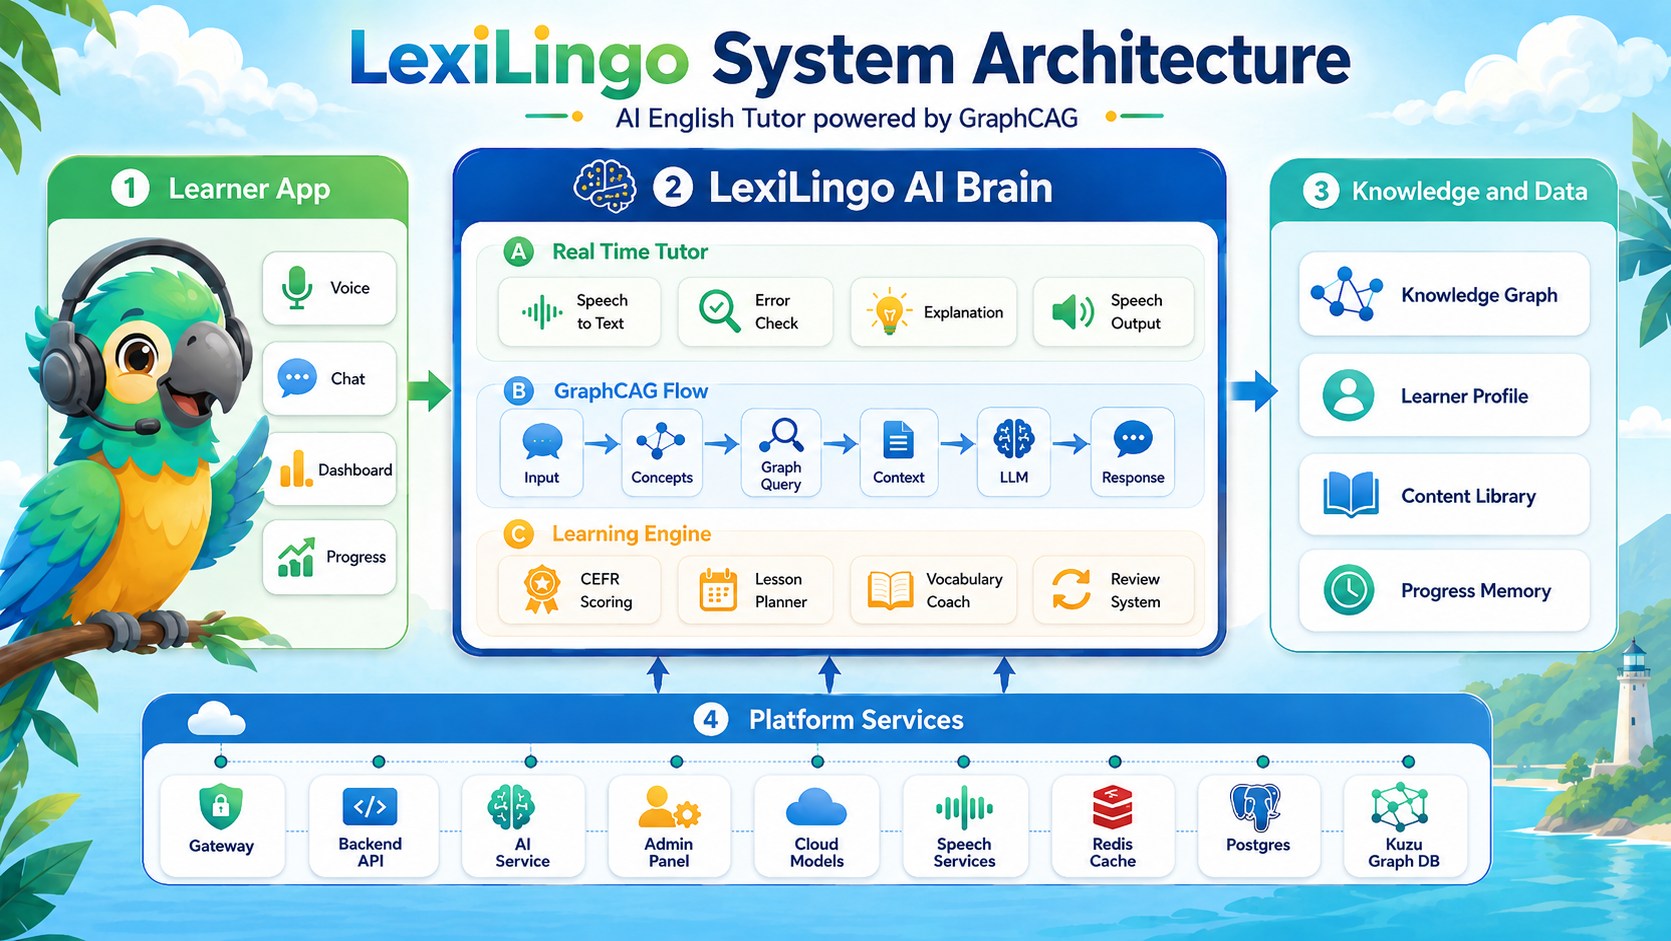
\includegraphics[width=\textwidth]{../architecture_lexilingo.png}
\caption{Kiến trúc tổng thể LexiLingo: tầng client, gateway, dịch vụ và dữ liệu}
\end{figure}

Mô tả theo tầng:

\begin{longtable}{L{2.8cm} L{11.0cm}}
\toprule
\textbf{Tầng} & \textbf{Thành phần và vai trò}\\
\midrule
\endhead
Client & Ứng dụng Flutter (người học), trang quản trị React (quản trị viên), MCP client (lập trình viên/tác tử AI trong IDE).\\
Gateway & Nginx 1.27-alpine: kết thúc TLS, định tuyến \code{/api/v1/*} về backend và \code{/ai/*} về AI service, giới hạn tần suất, chặn theo \en{WAF} biên (Cloudflare).\\
Dịch vụ & \code{backend-service} (cổng 8000) — nghiệp vụ; \code{ai-service} (cổng 8080) — AI; hai tiến trình phụ \code{backend-reminder-worker} và \code{backend-reminder-beat} chạy Celery.\\
Dữ liệu & PostgreSQL (nguồn sự thật nghiệp vụ), Redis (bộ nhớ đệm, phiên, hàng đợi Celery, bộ nhớ đệm đồ thị con), MongoDB (hội thoại, tạo tác AI, vùng đệm quan sát), KuzuDB (đồ thị tri thức nhúng).\\
Quan trắc & Prometheus thu thập chỉ số, Grafana hiển thị; nhật ký có \code{X-Request-ID} xuyên suốt.\\
\bottomrule
\caption{Các tầng trong kiến trúc}
\end{longtable}

\section{Luồng một yêu cầu điển hình}

Ví dụ: người học hoàn thành một bài học.

\begin{enumerate}[leftmargin=1.4em]
  \item Flutter gọi \code{POST /api/v1/learning/lessons/\{id\}/complete} kèm
  \en{JWT} (\en{JSON Web Token} — thẻ xác thực có chữ ký) trong tiêu đề \code{Authorization}.
  \item Nginx kiểm tra tần suất, gắn \code{X-Request-ID}, chuyển tiếp về backend.
  \item Backend chạy chuỗi \en{middleware}: kiểm tra máy chủ tin cậy $\rightarrow$ CORS
  $\rightarrow$ giới hạn tần suất $\rightarrow$ sinh mã yêu cầu $\rightarrow$ ghi nhật ký.
  \item Bộ định tuyến giải mã JWT, nạp người dùng, kiểm tra quyền.
  \item Tầng dịch vụ ghi \code{LessonCompletion}, cộng XP (\code{xp\_service}), cập nhật
  chuỗi ngày học (\code{streak\_service}), kiểm tra thành tích
  (\code{achievement\_checker\_service}).
  \item Kết quả từng bài tập được đẩy vào \code{record\_exercise\_results\_for\_user}:
  cập nhật \code{UserSkillScore} (điểm kỹ năng CEFR) và, nếu bài tập có
  \code{concept\_id}, gọi tiếp \code{record\_concept\_observation} để lập lịch ôn tập FSRS.
  \item Phản hồi trả về client; các tác vụ chậm (thông báo đẩy, tổng hợp thống kê) được
  đưa sang Celery.
\end{enumerate}

\begin{luuy}[Vì sao tách hai động cơ]
Điểm kỹ năng trả lời câu hỏi \textit{"người học đang ở bậc CEFR nào?"}; trạng thái khái
niệm trả lời \textit{"khi nào cần ôn lại khái niệm này?"}. Hai câu hỏi này có chu kỳ cập
nhật và ngữ nghĩa khác nhau, nên gộp chung sẽ làm hỏng cả hai. Điều bắt buộc là mọi hoạt
động có chấm điểm phải đến được cả hai động cơ.
\end{luuy}

\section{Ranh giới trách nhiệm giữa backend và AI service}

Đây là ranh giới hay bị hiểu nhầm nhất, nên được nêu rõ:

\begin{longtable}{L{6.8cm} L{6.8cm}}
\toprule
\textbf{backend-service} & \textbf{ai-service}\\
\midrule
\endhead
Nguồn sự thật về người học: tài khoản, tiến độ, XP, từ vựng, khoá học, trạng thái khái niệm. &
Không sở hữu dữ liệu người học; đọc/ghi qua API nội bộ của backend.\\
PostgreSQL là kho chính. & MongoDB (hội thoại, tạo tác), KuzuDB (đồ thị tri thức dùng chung), Redis (đệm).\\
Quyết định thăng bậc CEFR, mở khoá nội dung, trao thưởng. & Quyết định nội dung phản hồi, chiến lược sư phạm, chẩn đoán lỗi.\\
Mất dịch vụ $\Rightarrow$ mất khoá học, đăng nhập, tiến độ. & Mất dịch vụ $\Rightarrow$ mất chat/dịch/giọng nói, \textbf{không} mất tiến độ.\\
Thời gian dựng lại ảnh Docker: khoảng 1 phút. & Khoảng 15--30 phút (bánh xe \code{llama-cpp-python}).\\
\bottomrule
\caption{Ranh giới trách nhiệm giữa hai dịch vụ lõi}
\end{longtable}

\section{Hợp đồng dữ liệu dùng chung}

Thư mục \code{contracts/} chứa các định nghĩa dữ liệu mà nhiều dịch vụ cùng dựa vào.
Trường hợp điển hình là \textbf{danh sách khoá được phép} (\en{allowlist}) của tải trọng
quan sát người học: nó được khai báo hai nơi — \code{app/schemas/learner\_state.py} phía
backend và \code{api/services/learner\_observation\_spool.py} phía AI service. Một khoá lạ
sẽ làm cả lô quan sát bị từ chối, nên khi thêm trường mới phải sửa đồng thời cả hai; bộ
kiểm thử \code{test\_content\_contract\_parity.py} tồn tại để chặn việc quên.

\chapter{Thiết kế hệ thống}

\section{Sơ đồ use case hệ thống}

So với use case nghiệp vụ ở Chương~2 (điều người dùng \textit{muốn}), use case hệ thống
gắn nghiệp vụ với cơ chế kỹ thuật cụ thể (điều hệ thống \textit{làm}) và biểu diễn quan hệ
\en{include}/\en{extend} giữa chúng.

\begin{figure}[htbp]
\centering
\begin{tikzpicture}[scale=0.92, transform shape]
  \node[lane, minimum width=9.6cm, minimum height=9.6cm] (sys) at (0,0) {};
  \node[font=\scriptsize\bfseries, anchor=north, yshift=-3pt] at (sys.north) {Backend + AI service};

  \node[uc] (uc1) at (-2.6, 3.6) {Đăng nhập};
  \node[uc] (uc2) at ( 2.6, 3.6) {Xác thực JWT};
  \node[uc] (uc3) at (-2.6, 2.4) {Hoàn thành bài học};
  \node[uc] (uc4) at ( 2.6, 2.4) {Ghi nhận điểm CEFR};
  \node[uc] (uc5) at (-2.6, 1.2) {Ôn từ vựng};
  \node[uc] (uc6) at ( 2.6, 1.2) {Lập lịch FSRS};
  \node[uc] (uc7) at (-2.6, 0.0) {Chat với Lexi};
  \node[uc] (uc8) at ( 2.6, 0.0) {Chạy pipeline TRACE-CAG};
  \node[uc] (uc9) at (-2.6,-1.2) {Luyện nói};
  \node[uc] (uc10) at ( 2.6,-1.2) {STT + phân tích âm vị};
  \node[uc] (uc11) at (-2.6,-2.4) {Xem tiến độ};
  \node[uc] (uc12) at ( 2.6,-2.4) {Đọc \code{skill\_daily\_stats}};
  \node[uc, fill=cSoftO, draw=cGate] (uc13) at (-2.6,-3.6) {Xuất bản khoá học};
  \node[uc, fill=cSoftO, draw=cGate] (uc14) at ( 2.6,-3.6) {Kiểm tra \code{publish\_blockers}};

  \draw[fl, dashed] (uc1) -- node[lab]{«include»} (uc2);
  \draw[fl, dashed] (uc3) -- node[lab]{«include»} (uc4);
  \draw[fl, dashed] (uc5) -- node[lab]{«include»} (uc6);
  \draw[fl, dashed] (uc7) -- node[lab]{«include»} (uc8);
  \draw[fl, dashed] (uc9) -- node[lab]{«include»} (uc10);
  \draw[fl, dashed] (uc11) -- node[lab]{«include»} (uc12);
  \draw[fl, dashed] (uc13) -- node[lab]{«include»} (uc14);
  \draw[fl, dashed, draw=cGate] (uc8) .. controls (0.5,0.9) .. (uc4);
  \node[lab, draw=cGate, text=cGate, rotate=28] at (0.55,0.75) {«extend»};

  \stickman{-5.4}{1.4}{Người học}
  \stickman{-5.4}{-3.6}{Quản trị viên}
  \stickman{5.4}{-1.2}{Whisper /\\HuBERT}
  \stickman{5.4}{2.4}{PostgreSQL}

  \foreach \t in {uc1,uc3,uc5,uc7,uc9,uc11}
    \draw[draw=cInfra!60, line width=0.5pt] (-5.15,1.4) -- (\t.west);
  \draw[draw=cGate!70, line width=0.5pt] (-5.15,-3.6) -- (uc13.west);
  \draw[draw=cInfra!60, line width=0.5pt] (uc10.east) -- (5.15,-1.2);
  \draw[draw=cInfra!60, line width=0.5pt] (uc4.east) -- (5.15,2.4);
  \draw[draw=cInfra!60, line width=0.5pt] (uc6.east) -- (5.15,2.4);
  \draw[draw=cInfra!60, line width=0.5pt] (uc12.east) -- (5.15,2.4);
\end{tikzpicture}
\caption{Sơ đồ use case hệ thống — quan hệ \en{include}/\en{extend} giữa use case nghiệp vụ và cơ chế kỹ thuật}
\label{fig:uc-hethong}
\end{figure}

\section{Sơ đồ thực thể quan hệ (ERD)}

ERD dưới đây chỉ vẽ các thực thể trung tâm và khoá ngoại giữa chúng — bảng dữ liệu đầy đủ
(khoảng 70 bảng) nằm ở Chương~6. Mọi khoá ngoại trỏ về người dùng đều
\codesp{ON DELETE CASCADE} trừ khi ghi chú khác.

\begin{figure}[htbp]
\centering
\resizebox{\textwidth}{!}{
\begin{tikzpicture}[node distance=15mm]
  \node[ent] (user) {\textbf{User}\\[2pt] id (PK)\\ email\\ password\_hash\\ role};
  \node[ent, right=28mm of user] (course) {\textbf{Course}\\[2pt] id (PK)\\ title\\ cefr\_level\\ status};
  \node[ent, below=of course] (unit) {\textbf{Unit}\\[2pt] id (PK)\\ course\_id (FK)\\ order};
  \node[ent, below=of unit] (lesson) {\textbf{Lesson}\\[2pt] id (PK)\\ unit\_id (FK)\\ content (JSON)\\ exercise\_count};

  \node[ent, below=of user] (progress) {\textbf{UserCourseProgress}\\[2pt] id (PK)\\ user\_id (FK)\\ course\_id (FK)};
  \node[ent, below=of progress] (completion) {\textbf{LessonCompletion}\\[2pt] id (PK)\\ user\_id (FK)\\ lesson\_id (FK)\\ score};

  \node[ent, right=28mm of lesson] (concept) {\textbf{LearnerConceptState}\\[2pt] user\_id (FK)\\ concept\_id\\ mastery\_probability\\ stability\_days\\ next\_review\_at};
  \node[ent, above=of concept] (obsevt) {\textbf{LearnerObservationEvent}\\[2pt] event\_id (UNIQUE)\\ user\_id (FK)\\ concept\_id\\ status};
  \node[ent, right=28mm of concept] (profile) {\textbf{LearnerStateProfile}\\[2pt] user\_id (PK, FK)\\ state\_epoch};

  \node[ent, below=of completion] (skill) {\textbf{UserSkillScore}\\[2pt] id (PK)\\ user\_id (FK)\\ skill\\ score\\ confidence};
  \node[ent, below=of skill] (attempt) {\textbf{ExerciseAttempt}\\[2pt] id (PK)\\ user\_id (FK)\\ skill\\ score\\ (cắt tỉa 90 ngày)};
  \node[ent, right=28mm of attempt] (daily) {\textbf{SkillDailyStat}\\[2pt] user\_id (FK)\\ day\\ skill\\ score\_avg};

  \node[ent, right=28mm of daily] (xp) {\textbf{XPTransaction}\\[2pt] id (PK)\\ user\_id (FK)\\ source\\ source\_id\\ amount};

  \draw[fl] (course.south) -- (unit.north);
  \draw[fl] (unit.south) -- (lesson.north);
  \draw[fl] (user.south) -- (progress.north);
  \draw[fl] (progress.south) -- (completion.north);
  \draw[fl] (completion.east) -- (lesson.west);
  \draw[fl] (progress.east) -- (course.west);
  \draw[fl] (obsevt.south) -- (concept.north);
  \draw[fl] (concept.east) -- (profile.west);
  \draw[fl] (user.south) .. controls (2,-6) .. (obsevt.west);
  \draw[fl] (completion.south) -- (skill.north);
  \draw[fl] (skill.south) -- (attempt.north);
  \draw[fl] (attempt.east) -- (daily.west);
  \draw[fl] (daily.east) -- (xp.west);
  \draw[fl] (user.south) .. controls (10,2) and (10,-8) .. (xp.north);
\end{tikzpicture}}
\caption{ERD rút gọn — quan hệ giữa nội dung khoá học, tiến độ và hai động cơ mô hình người học}
\label{fig:erd}
\end{figure}

\begin{luuy}[Vì sao \code{LearnerStateProfile} tách khỏi \code{LearnerConceptState}]
Mỗi người học có nhiều dòng \code{LearnerConceptState} (một cho mỗi khái niệm đã học) nhưng
chỉ có \textbf{một} dòng \code{LearnerStateProfile}. Tách riêng để tăng \code{state\_epoch}
là một phép ghi một dòng duy nhất, không phải cập nhật hàng loạt — đây là điều kiện để vô
hiệu hoá bộ đệm cá nhân hoá diễn ra tức thời và rẻ (Chương~9).
\end{luuy}

\section{Sơ đồ lớp — lõi mô hình người học}

\begin{figure}[htbp]
\centering
\begin{tikzpicture}[node distance=8mm and 14mm]
  \node[ent, align=left] (svc) {\textbf{learner\_state.py}\\[2pt]
    + evolve\_state(state, outcome,\\ \ \ confidence, now)\\
    + grade\_to\_observation(quality)\\
    - \_retrievability(t, S)\\
    - \_interval\_days(S)\\
    - \_initial\_stability(outcome, c)};
  \node[ent, align=left, right=of svc] (snap) {\textbf{LearnerStateSnapshot}\\[2pt]
    mastery\_probability: float\\
    stability\_days: float\\
    difficulty: float\\
    attempt/correct/error\_count: int\\
    last\_interacted\_at: datetime\\
    algorithm\_version: str};
  \node[ent, align=left, below=of svc] (model) {\textbf{LearnerConceptState (ORM)}\\[2pt]
    user\_id, concept\_id: PK\\
    + mọi trường của Snapshot\\
    state\_version: int};
  \node[ent, align=left, below=of snap] (input) {\textbf{ObservationInput}\\[2pt]
    event\_id: str (UNIQUE)\\
    user\_id, concept\_id: str\\
    outcome: "correct"|"incorrect"\\
    confidence: float\\
    session\_id, payload};

  \draw[fl] (svc) -- node[lab,above]{tạo/đọc} (snap);
  \draw[fl] (model.north) -- node[lab,left]{\_snapshot\_from\_model} (svc.south);
  \draw[fl] (input) -- node[lab,below]{nạp vào} (svc);
  \draw[fl, dashed] (snap.south) -- node[lab,right]{\_apply\_snapshot} (model.east |- snap.south);
\end{tikzpicture}
\caption{Sơ đồ lớp — hàm thuần \code{evolve\_state} tách khỏi lớp ORM để kiểm thử không phụ thuộc cơ sở dữ liệu}
\label{fig:class-learnerstate}
\end{figure}

Thiết kế tách \code{LearnerStateSnapshot} (bất biến, không phụ thuộc cơ sở dữ liệu) khỏi
\code{LearnerConceptState} (ORM, có trạng thái) là có chủ đích: hàm \code{evolve\_state}
là một hàm thuần — cùng đầu vào luôn cho cùng đầu ra — nên kiểm thử được bằng
\code{assert} thuần tuý mà không cần dựng cơ sở dữ liệu. Tầng gọi (\code{record\_concept\_observation})
mới chịu trách nhiệm đọc/ghi ORM.

\section{Sơ đồ tuần tự}

\subsection{Hoàn thành bài học — đường đi hai động cơ}

\begin{figure}[htbp]
\centering
\begin{tikzpicture}[
  actor/.style={rectangle, draw=cInfra, fill=cSoftGray, rounded corners=2pt,
                minimum height=6mm, font=\scriptsize, align=center},
  seq/.style={-{Stealth[length=3.5pt]}, draw=cInfra!80, line width=0.5pt, font=\tiny},
  seqret/.style={{Stealth[length=3.5pt]}-, draw=cInfra!50, dashed, line width=0.5pt, font=\tiny},
  ]
  \node[actor] (a0) at (0,0) {Flutter};
  \node[actor] (a1) at (2.3,0) {Route\\\code{/learning}};
  \node[actor] (a2) at (4.6,0) {\code{xp\_service}};
  \node[actor] (a3) at (6.9,0) {\code{proficiency\_service}};
  \node[actor] (a4) at (9.2,0) {\code{learner\_state}};
  \node[actor] (a5) at (11.5,0) {PostgreSQL};

  \foreach \a in {a0,a1,a2,a3,a4,a5}
    \draw[draw=cInfra!40, line width=0.4pt] (\a.south) -- ++(0,-8.2);

  \draw[seq] ([yshift=-0.8cm]a0.south) -- node[lab,above]{POST attempts/complete} ([yshift=-0.8cm]a1.south);
  \draw[seq] ([yshift=-1.4cm]a1.south) -- node[lab,above]{award\_xp\_transaction} ([yshift=-1.4cm]a2.south);
  \draw[seqret] ([yshift=-1.9cm]a2.south) -- node[lab,above]{xp\_awarded} ([yshift=-1.9cm]a1.south);
  \draw[seq] ([yshift=-2.5cm]a1.south) -- node[lab,above]{record\_exercise\_results\_for\_user} ([yshift=-2.5cm]a3.south);
  \draw[seq] ([yshift=-3.1cm]a3.south) -- node[lab,above]{cập nhật EMA} ([yshift=-3.1cm]a5.south);
  \draw[seq] ([yshift=-3.7cm]a3.south) -- node[lab,above]{record\_concept\_observation (nếu có concept\_id)} ([yshift=-3.9cm]a4.south);
  \draw[seq] ([yshift=-4.6cm]a4.south) -- node[lab,above]{evolve\_state + ghi} ([yshift=-4.6cm]a5.south);
  \draw[seqret] ([yshift=-5.2cm]a5.south) -- node[lab,above]{state\_epoch++} ([yshift=-5.2cm]a4.south);
  \draw[seqret] ([yshift=-5.8cm]a3.south) -- node[lab,above]{kết quả} ([yshift=-5.8cm]a1.south);
  \draw[seqret] ([yshift=-6.4cm]a1.south) -- node[lab,above]{200 OK} ([yshift=-6.4cm]a0.south);
\end{tikzpicture}
\caption{Sơ đồ tuần tự — hoàn thành bài học chạm cả hai động cơ mô hình người học trong cùng một yêu cầu}
\label{fig:seq-lesson}
\end{figure}

\subsection{Hội thoại AI — dòng SSE và ghi quan sát}

\begin{figure}[htbp]
\centering
\begin{tikzpicture}[
  actor/.style={rectangle, draw=cInfra, fill=cSoftGray, rounded corners=2pt,
                minimum height=6mm, font=\scriptsize, align=center},
  seq/.style={-{Stealth[length=3.5pt]}, draw=cInfra!80, line width=0.5pt, font=\tiny},
  seqret/.style={{Stealth[length=3.5pt]}-, draw=cInfra!50, dashed, line width=0.5pt, font=\tiny},
  ]
  \node[actor] (a0) at (0,0)    {Flutter};
  \node[actor] (a1) at (2.4,0)  {\code{lexi\_chat.py}};
  \node[actor] (a2) at (4.8,0)  {TRACE-CAG\\StateGraph};
  \node[actor] (a3) at (7.2,0)  {LLM\\(Groq/Gemini)};
  \node[actor] (a4) at (9.6,0)  {Mongo\\spool};
  \node[actor] (a5) at (12.0,0) {Backend\\\code{learner\_state}};

  \foreach \a in {a0,a1,a2,a3,a4,a5}
    \draw[draw=cInfra!40, line width=0.4pt] (\a.south) -- ++(0,-6.6);

  \draw[seq] ([yshift=-0.7cm]a0.south) -- node[lab,above]{SSE: gửi câu} ([yshift=-0.7cm]a1.south);
  \draw[seq] ([yshift=-1.3cm]a1.south) -- node[lab,above]{analyze()} ([yshift=-1.3cm]a2.south);
  \node[lab, fill=cSoft, draw=cService, rounded corners=1pt] at ([yshift=-2.0cm,xshift=6mm]a2.south) {diagnose + retrieve};
  \draw[seq] ([yshift=-2.5cm]a2.south) -- node[lab,above]{sinh phản hồi (dòng)} ([yshift=-2.5cm]a3.south);
  \draw[seqret] ([yshift=-3.1cm]a3.south) -- node[lab,above]{token} ([yshift=-3.1cm]a2.south);
  \draw[seq] ([yshift=-3.7cm]a2.south) -- node[lab,above]{event: chunk} ([yshift=-3.7cm]a1.south);
  \draw[seq] ([yshift=-4.0cm]a1.south) -- node[lab,above]{} ([yshift=-4.0cm]a0.south);
  \draw[seq] ([yshift=-4.7cm]a2.south) -- node[lab,above]{bulk upsert quan sát} ([yshift=-4.7cm]a4.south);
  \draw[seqret] ([yshift=-5.2cm]a4.south) -- node[lab,above]{ACK} ([yshift=-5.2cm]a2.south);
  \draw[seq] ([yshift=-5.7cm]a2.south) -- node[lab,above]{event: done} ([yshift=-5.7cm]a1.south);
  \draw[seq] ([yshift=-6.0cm]a1.south) -- node[lab,above]{} ([yshift=-6.0cm]a0.south);
  \draw[seq, dashed, draw=cGate] ([yshift=-6.5cm]a4.south) -- node[lab,above,text=cGate]{lease worker (bất đồng bộ)} ([yshift=-6.5cm]a5.south);
\end{tikzpicture}
\caption{Sơ đồ tuần tự — quan sát được ghi vào vùng đệm \textbf{trước} dấu \code{done}, việc chuyển sang backend là bất đồng bộ}
\label{fig:seq-chat}
\end{figure}

\section{Sơ đồ triển khai}

\begin{figure}[htbp]
\centering
\begin{tikzpicture}[scale=0.9, transform shape]
  \node[lane, minimum width=11.6cm, minimum height=8.4cm] (vps) at (0,0) {};
  \node[font=\scriptsize\bfseries, anchor=north, yshift=-3pt] at (vps.north) {Máy chủ ảo — /opt/lexilingo};

  \node[gat] (gw) at (0,3.2) {Nginx 1.27\\:80 / :443};

  \node[svc] (be) at (-3.6,1.6) {backend-service\\FastAPI :8000};
  \node[svc] (ai) at (0,1.6) {ai-service\\FastAPI :8080};
  \node[inf] (adm) at (3.6,1.6) {admin (Vercel)\\ngoài VPS};

  \node[svc] (wk) at (-3.6,0.1) {reminder-worker\\Celery};
  \node[svc] (bt) at (0,0.1) {reminder-beat\\Celery};

  \node[dat] (pg) at (-4.2,-1.6) {PostgreSQL};
  \node[dat] (rd) at (-1.4,-1.6) {Redis};
  \node[dat] (mg) at (1.4,-1.6) {MongoDB};
  \node[dat] (kz) at (4.2,-1.6) {KuzuDB\\(nhúng)};

  \node[inf] (pr) at (-2.4,-3.2) {Prometheus};
  \node[inf] (gr) at (2.4,-3.2) {Grafana};

  \draw[fl] (gw) -- (be); \draw[fl] (gw) -- (ai);
  \draw[flb] (be) -- (ai);
  \draw[fl] (wk) -- (rd); \draw[fl] (bt) -- (rd);
  \draw[fl] (be) -- (pg); \draw[fl] (be) -- (rd);
  \draw[fl] (ai) -- (mg); \draw[fl] (ai) -- (kz); \draw[fl] (ai) -- (rd);
  \draw[fl] (be) -- (pr); \draw[fl] (ai) -- (pr);
  \draw[fl] (pr) -- (gr);
  \draw[fl, dashed, draw=cInfra] (gw) .. controls (5.5,3.5) and (5.5,1.8) .. (adm);

  \stickman{-6.6}{2.8}{Flutter\\(Android/iOS/Web)}
  \draw[fl] (-6.2,2.55) -- (gw.west);
\end{tikzpicture}
\caption{Sơ đồ triển khai sản xuất — một VPS chạy Docker Compose, admin triển khai riêng trên Vercel}
\label{fig:deploy}
\end{figure}

\section{Đặc tả use case chi tiết — hai use case trung tâm}

\begin{longtable}{L{3.2cm} L{9.6cm}}
\toprule
\multicolumn{2}{l}{\textbf{UC-01 — Hoàn thành bài học}}\\
\midrule
\endhead
Tác nhân chính & Người học\\
Điều kiện trước & Đã đăng nhập; bài học có \code{exercise\_count} $>0$\\
Luồng chính & 1. Người học mở bài học. 2. Trả lời tuần tự các bài tập. 3. Hệ thống chấm điểm từng câu theo hình dạng bài tập (Chương~5). 4. Nộp lượt làm. 5. Hệ thống ghi \code{LessonCompletion}, cộng XP, cập nhật điểm kỹ năng, lập lịch FSRS cho khái niệm liên quan, kiểm tra thành tích.\\
Luồng phụ & 3a. Bài học không có bài tập $\rightarrow$ hệ thống trả lỗi 409 ngay ở bước mở bài, không cho vào luồng chính.\\
Điều kiện sau & \code{UserSkillScore}, \code{LearnerConceptState}, \code{XPTransaction} đều được cập nhật trong cùng luồng xử lý yêu cầu.\\
\bottomrule
\end{longtable}

\begin{longtable}{L{3.2cm} L{9.6cm}}
\toprule
\multicolumn{2}{l}{\textbf{UC-02 — Hội thoại với trợ lý AI}}\\
\midrule
\endhead
Tác nhân chính & Người học\\
Tác nhân phụ & Nhà cung cấp LLM\\
Điều kiện trước & Đã đăng nhập; có phiên hội thoại hoặc phiên mới được tạo\\
Luồng chính & 1. Người học gửi câu. 2. Hệ thống kiểm tra bộ đệm hai lớp. 3. Nếu trượt: mở rộng đồ thị và chẩn đoán song song. 4. Truy xuất bằng chứng. 5. Sinh phản hồi theo chiến lược sư phạm phù hợp bậc. 6. Ghi quan sát học tập vào vùng đệm \textbf{trước} khi trả lời. 7. Trả phản hồi theo dòng SSE.\\
Luồng phụ & 3a. Độ tin cậy chẩn đoán $<0{,}5$ $\rightarrow$ hỏi làm rõ, bỏ qua bước 4--5. \newline 2a. Đệm trúng $\rightarrow$ bỏ qua bước 3--6, trả thẳng phản hồi đã lưu.\\
Điều kiện sau & Một khoản mục đệm mới được ghi (nếu tính lại); \code{learner\_observation\_spool} có thêm sự kiện.\\
\bottomrule
\end{longtable}

\chapter{Backend service — nghiệp vụ và API}

\section{Tổ chức mã nguồn}

\begin{longtable}{L{4.0cm} L{9.6cm}}
\toprule
\textbf{Thư mục} & \textbf{Nội dung}\\
\midrule
\endhead
\code{app/main.py} & Điểm vào ứng dụng: đăng ký \en{middleware}, bộ định tuyến, bộ xử lý ngoại lệ, vòng đời khởi động/tắt.\\
\code{app/core/} & Cấu hình (\code{config.py}), động cơ cơ sở dữ liệu bất đồng bộ, bảo mật (băm mật khẩu, JWT), xác thực Firebase, phụ thuộc FastAPI, \en{middleware}, Redis, bộ nhớ đệm, Celery.\\
\code{app/models/} & 25 tệp mô hình ORM SQLAlchemy, khoảng 70 bảng.\\
\code{app/schemas/} & Lược đồ Pydantic v2 — hợp đồng đầu vào/ra của API.\\
\code{app/routes/} & 41 mô-đun định tuyến.\\
\code{app/services/} & 45 dịch vụ nghiệp vụ (không chứa mã HTTP).\\
\code{app/crud/} & Lớp truy cập dữ liệu tái sử dụng cho 8 miền lớn.\\
\code{app/clients/} & \code{ai\_service\_client.py} — cửa duy nhất gọi sang AI service.\\
\code{app/tasks/} & 9 mô-đun tác vụ nền Celery.\\
\code{alembic/} & Di trú lược đồ cơ sở dữ liệu.\\
\code{scripts/} & Gieo dữ liệu, kiểm toán nội dung, sinh bài tập bằng AI, sao lưu.\\
\bottomrule
\caption{Cấu trúc thư mục backend-service}
\end{longtable}

\section{Chuỗi middleware}

\en{Middleware} là lớp bọc quanh ứng dụng: yêu cầu đi vào phải xuyên qua từ ngoài vào
trong, phản hồi đi ra xuyên qua theo chiều ngược lại. Thứ tự đăng ký quyết định thứ tự
chạy — lớp đăng ký sau cùng nằm ngoài cùng.

\begin{center}
\code{PrivateNetworkAccess $\rightarrow$ CORS $\rightarrow$ RateLimit $\rightarrow$ RequestID $\rightarrow$ RequestLogging $\rightarrow$ App}
\end{center}

\begin{longtable}{L{4.6cm} L{9.0cm}}
\toprule
\textbf{Lớp} & \textbf{Chức năng}\\
\midrule
\endhead
\code{TrustedHostMiddleware} & Chỉ chấp nhận yêu cầu có tiêu đề \code{Host} nằm trong danh sách cho phép; chỉ bật ở môi trường sản xuất.\\
\code{PrivateNetworkAccess} & Gắn tiêu đề CORS-RFC1918 để trình duyệt Chrome cho phép truy cập mạng nội bộ trong lúc phát triển.\\
\code{CORSMiddleware} & Kiểm soát nguồn gốc chéo (\en{cross-origin}) — chỉ cho phép miền \code{lexilingo.me} và các nguồn cấu hình.\\
\code{RateLimitMiddleware} & Cửa sổ trượt trên Redis; mặc định 300 yêu cầu/phút khi phát triển và 120 khi sản xuất, trần 5.000/giờ.\\
\code{RequestIDMiddleware} & Sinh \code{X-Request-ID} để lần vết một yêu cầu qua toàn bộ nhật ký. Tác vụ Celery cũng nhận mã tương tự dạng \code{task:\{id\}}.\\
\code{RequestLoggingMiddleware} & Ghi phương thức, đường dẫn, mã trạng thái và độ trễ.\\
\code{limit\_request\_body} & Từ chối thân yêu cầu vượt \code{MAX\_REQUEST\_BODY\_BYTES}.\\
\bottomrule
\caption{Chuỗi middleware của backend}
\end{longtable}

\section{Nhóm định tuyến}

Toàn bộ API dùng tiền tố \code{/api/v1}. Bốn mươi mốt mô-đun được nhóm theo miền:

\begin{longtable}{L{3.9cm} L{9.7cm}}
\toprule
\textbf{Nhóm} & \textbf{Mô-đun và chức năng}\\
\midrule
\endhead
Xác thực \& người dùng & \code{auth} (đăng ký, đăng nhập, làm mới thẻ, Google/Facebook qua Firebase, quên/đổi mật khẩu), \code{users} (hồ sơ, tuỳ chọn, ảnh đại diện), \code{devices} (đăng ký thiết bị nhận thông báo đẩy), \code{rbac} (vai trò, quyền), \code{entitlements} (quyền lợi gói trả phí), \code{referral} (giới thiệu bạn bè).\\
Nội dung học & \code{courses}, \code{course\_categories}, \code{learning} (phiên học, bắt đầu/hoàn thành bài), \code{vocabulary} (ngân hàng từ, ôn tập), \code{concepts} (khái niệm tri thức), \code{mistakes} (sổ tay lỗi sai).\\
Tiến độ \& năng lực & \code{progress} (tiến độ, chuỗi ngày, hoạt động hằng ngày), \code{proficiency} (đánh giá CEFR sáu kỹ năng, cổng thi thăng bậc), \code{learner\_state} (điểm vào nội bộ cho quan sát từ AI service).\\
Động lực học & \code{gamification} (thành tích, ví, cửa hàng, kho đồ, bảng xếp hạng), \code{xp} (giao dịch điểm kinh nghiệm), \code{challenges} (thử thách), \code{games} (trò chơi mini — mô-đun lớn nhất).\\
Nội dung thực tế & \code{news}, \code{podcasts}, \code{books}, \code{youtube} — nội dung ngoài đời thực kèm câu hỏi/quiz.\\
Thông báo & \code{notifications}, \code{reminders} (tuỳ chọn nhắc học), \code{notification\_campaign} (chiến dịch gửi hàng loạt).\\
Tác tử AI & \code{content\_agent} (sinh khoá học), \code{ranking\_agent} (xếp hạng, giải đấu), \code{admin\_ai\_proxy} (uỷ nhiệm gọi AI service từ trang quản trị), \code{ai\_audit} (nhật ký quyết định AI).\\
Quản trị \& vận hành & \code{admin\_courses}, \code{admin\_gamification}, \code{admin\_system}, \code{user\_management}, \code{analytics}, \code{monitoring}, \code{product\_events}, \code{integrations}, \code{health}, \code{well\_known}.\\
\bottomrule
\caption{Bốn mươi mốt mô-đun định tuyến theo miền}
\end{longtable}

\section{Xác thực và phân quyền}

\subsection{Luồng xác thực}

Hệ thống hỗ trợ ba đường đăng nhập, tất cả cùng quy về một loại thẻ nội bộ:

\begin{enumerate}[leftmargin=1.4em]
  \item \textbf{Email/mật khẩu} — mật khẩu băm bằng \code{bcrypt} gọi trực tiếp
  (\code{bcrypt.hashpw}), không qua \code{passlib} vì thư viện này có lỗi tương thích với
  bcrypt 4.x.
  \item \textbf{Google / Facebook} — client lấy thẻ Firebase, backend xác minh bằng
  Firebase Admin SDK rồi phát hành JWT của chính hệ thống.
  \item \textbf{Đối tác} — khoá API lưu ở bảng \code{partner\_api\_keys}.
\end{enumerate}

Thẻ truy cập (\en{access token}) có tuổi thọ ngắn, thẻ làm mới (\en{refresh token}) lưu ở
bảng \code{refresh\_tokens} và có thể thu hồi. Ứng dụng Flutter chủ động làm mới
\textbf{trước khi} thẻ hết hạn thay vì đợi lỗi 401 — thay đổi này (commit
\code{557d29c4}) vừa giảm độ trễ vừa cắt chi phí gọi Firebase.

\subsection{Phân quyền theo vai trò}

Bốn bảng \code{roles}, \code{permissions}, \code{role\_permissions} và \code{audit\_logs}
tạo nên hệ RBAC đầy đủ. Quyền được kiểm tra bằng \en{dependency} của FastAPI, tức là khai
báo ngay trên chữ ký hàm định tuyến chứ không nằm rải rác trong thân hàm. Mọi thao tác
quản trị nhạy cảm ghi lại vào \code{audit\_logs}.

\section{Các dịch vụ nghiệp vụ chính}

\begin{longtable}{L{5.0cm} L{8.6cm}}
\toprule
\textbf{Dịch vụ} & \textbf{Trách nhiệm}\\
\midrule
\endhead
\code{proficiency\_service} & Chấm điểm sáu kỹ năng CEFR, tính điểm tổng hợp có trọng số, quyết định điều kiện thăng bậc. Xem Chương~9.\\
\code{learner\_state} & Tiến hoá trạng thái khái niệm theo FSRS + luật delta; điểm vào duy nhất \code{record\_concept\_observation}.\\
\code{learner\_state\_outbox} & Mẫu \en{outbox}: ghi sự kiện quan sát vào cùng giao dịch rồi mới xác nhận, tránh mất dữ liệu khi mạng đứt.\\
\code{fsrs\_scheduler\_service}, \code{game\_fsrs\_service} & Lập lịch ôn tập cho từ vựng và cho trò chơi.\\
\code{xp\_service} & Cấp điểm kinh nghiệm, áp trần theo ngày và theo nguồn, hệ số chuỗi ngày, chống cấp trùng.\\
\code{achievement\_checker\_service} & Kiểm tra và mở khoá thành tích theo \en{trigger} (sự kiện kích hoạt) thay vì quét toàn bộ.\\
\code{streak\_service} & Chuỗi ngày học liên tiếp, khiên bảo vệ chuỗi.\\
\code{rank\_service}, \code{ranking\_agent} & Xếp hạng, giải đấu theo tuần, đặt lại bảng xếp hạng.\\
\code{game\_scoring\_service} & Chấm điểm trò chơi, quy đổi sang kỹ năng CEFR tương ứng.\\
\code{content\_agent\_apply} & Đường duy nhất dựng khoá học $\rightarrow$ chương $\rightarrow$ bài học kèm bài tập từ kết quả của tác tử nội dung.\\
\code{content\_agent\_validation} & Làm sạch và kiểm tra hình dạng bài tập trước khi ghi.\\
\code{vocabulary\_catalog} & Danh mục từ vựng và chính sách chọn từ.\\
\code{skill\_history\_service} & Tổng hợp thống kê kỹ năng theo ngày; cắt tỉa nhật ký chi tiết.\\
\code{entitlement\_service}, \code{revenuecat\_client} & Quyền lợi gói trả phí, đồng bộ với RevenueCat.\\
\code{push\_notification\_service}, \code{reminder\_service} & Thông báo đẩy và nhắc học theo lịch FSRS.\\
\code{user\_deletion\_service} & Xoá tài khoản và dữ liệu liên quan theo yêu cầu quyền riêng tư.\\
\code{quota\_manager}, \code{api\_cache\_service} & Hạn ngạch gọi API theo người dùng; bộ nhớ đệm phản hồi trên Redis.\\
\bottomrule
\caption{Dịch vụ nghiệp vụ backend}
\end{longtable}

\section{Bất biến nội dung khoá học}

Một bài học chỉ \textbf{chơi được} khi \code{content.exercises} không rỗng. Bất biến này
được thực thi ở nhiều tầng, vì mỗi tầng từng bị vi phạm:

\begin{itemize}[leftmargin=1.4em]
  \item Cột \code{Lesson.exercise\_count} được đồng bộ tự động bằng \en{hook}
  \code{@validates("content")}; không được gán tay. Mọi câu hỏi "bài này học được chưa?"
  phải dùng cột này, không dùng \code{total\_exercises}.
  \item Các điểm cuối hướng người học (lộ trình, chi tiết khoá học) ẩn bài học rỗng;
  \code{/learning/lessons/\{id\}/start} và \code{/content} trả lỗi 409 ở môi trường sản xuất.
  \item Xuất bản khoá học bị chặn nếu còn bài học rỗng
  (\code{CourseCRUD.publish\_blockers}), chỉ kiểm tra tại thời điểm chuyển
  bản nháp $\rightarrow$ đã xuất bản.
  \item Mọi chỉnh sửa bài học từ trang quản trị đều đi qua \code{\_apply\_lesson\_update}
  — dùng chung bởi \code{PUT /lessons/\{id\}} và \code{PUT /lessons/\{id\}/content}.
\end{itemize}

\begin{luuy}[Hình dạng bài tập không được kiểm tra khi ghi]
Hệ thống kiểm tra "có bài tập hay không" nhưng không kiểm tra "bài tập có đúng hình dạng
không". Ba dạng đã từng hỏng: dạng ghép cặp phải nối bằng dấu \code{", "} vì bộ chấm tách
theo dấu phẩy; dạng \code{arrange\_the\_sentence} có đáp án \textbf{không} nằm trong danh
sách lựa chọn nên không dùng được phép kiểm tra chung; dạng \code{image\_based\_choice}
không có đường ống ảnh nên tuyệt đối không được sinh ra.
\end{luuy}

\section{Tác vụ nền Celery}

Celery chạy hai tiến trình riêng: \code{worker} (thực thi) và \code{beat} (hẹn giờ), dùng
Redis làm môi giới. Cấu hình đặt \code{task\_acks\_late=True} và
\code{worker\_prefetch\_multiplier=1} để tác vụ chỉ được xác nhận sau khi hoàn thành.

\begin{longtable}{L{5.6cm} L{3.2cm} L{4.6cm}}
\toprule
\textbf{Tác vụ} & \textbf{Lịch} & \textbf{Mục đích}\\
\midrule
\endhead
\code{scan\_fsrs\_reminders} & theo chu kỳ cấu hình & Tìm khái niệm đến hạn ôn, đẩy nhắc nhở.\\
\code{send\_streak\_alerts} & 20:00 hằng ngày & Cảnh báo sắp mất chuỗi ngày học.\\
\code{send\_word\_of\_day} & 08:00 hằng ngày & Từ vựng trong ngày.\\
\code{cleanup\_expired\_content\_agent\_uploads} & 03:15 hằng ngày & Dọn tệp tải lên hết hạn.\\
\code{cleanup\_learner\_observations} & 02:30 hằng ngày & Dọn quan sát đã áp dụng.\\
\code{prune\_exercise\_attempts} & 02:45 hằng ngày & Cắt nhật ký trả lời cũ hơn 90 ngày.\\
\code{snapshot\_skill\_scores} & 03:00 thứ Hai & Chụp ảnh điểm kỹ năng để tính xu hướng 7/30 ngày.\\
\code{auto\_league\_reset} & 00:05 thứ Hai & Đặt lại giải đấu tuần.\\
\code{prefetch\_news} & mỗi 6 giờ & Nạp trước tin tức.\\
\code{prefetch\_youtube} & mỗi 12 giờ & Nạp trước video.\\
\code{prefetch\_podcasts} & 00:00 hằng ngày & Nạp trước podcast.\\
\bottomrule
\caption{Lịch tác vụ nền}
\end{longtable}

\begin{luuy}[Vì sao có \code{snapshot\_skill\_scores}]
Cột \code{UserSkillScore.trend} đọc \code{score\_7d\_ago} và \code{score\_30d\_ago} —
hai cột mà trước đó \textbf{không có tiến trình nào ghi vào}. Xu hướng vì thế luôn bằng
không. Tác vụ tuần này là cách rẻ nhất để có lịch sử mà không cần thêm bảng lịch sử riêng.
\end{luuy}

\section{Xử lý lỗi}

Ba bộ xử lý ngoại lệ được đăng ký ở \code{main.py}, đảm bảo mọi lỗi trả về cùng một hình
dạng JSON:

\begin{lstlisting}[language=Python]
{
  "error": {
    "code": "VALIDATION_ERROR",
    "message": "...",
    "details": [ ... ]
  }
}
\end{lstlisting}

Nhờ vậy client chỉ cần một bộ phân tích lỗi duy nhất, và mã lỗi (\code{code}) là hằng số
ổn định để so khớp thay vì phải đọc thông điệp tiếng Anh.

\chapter{Tầng dữ liệu}

\section{Bốn kho lưu trữ và lý do tồn tại}

\begin{longtable}{L{2.6cm} L{4.0cm} L{7.0cm}}
\toprule
\textbf{Kho} & \textbf{Nội dung} & \textbf{Lý do chọn}\\
\midrule
\endhead
PostgreSQL & Tài khoản, khoá học, tiến độ, XP, từ vựng, trạng thái khái niệm — khoảng 70 bảng. &
Dữ liệu có quan hệ chặt, cần giao dịch (\en{transaction}) và ràng buộc toàn vẹn. Đây là \textbf{nguồn sự thật}.\\
Redis & Bộ nhớ đệm phản hồi, phiên, danh sách đen thẻ, hạn ngạch, môi giới Celery, đệm đồ thị con L0/L1. &
Đọc/ghi dưới mili-giây, cấu hình \code{allkeys-lru} nên có thể mất dữ liệu — vì vậy chỉ chứa thứ tái tạo được.\\
MongoDB & Lịch sử hội thoại, tạo tác AI, vùng đệm quan sát người học. &
Tài liệu không đồng nhất, ghi nhiều đọc ít, không cần \en{join}.\\
KuzuDB & Đồ thị tri thức: khái niệm, quan hệ tiên quyết/liên quan/dễ nhầm. &
Cơ sở dữ liệu đồ thị \textbf{nhúng} (không cần máy chủ riêng), tối ưu cho duyệt theo chiều rộng trên chuỗi tiên quyết.\\
\bottomrule
\caption{Bốn kho lưu trữ}
\end{longtable}

\begin{luuy}[Chỉ hai kho chứa dữ liệu người dùng]
Chính sách sao lưu chỉ bảo vệ PostgreSQL và MongoDB. Redis là bộ nhớ đệm và cố ý
\textbf{không} sao lưu; thư mục \code{ai\_models} và \code{content\_etl\_data} tải lại được.
\end{luuy}

\section{Nhóm bảng PostgreSQL theo miền}

\begin{longtable}{L{3.4cm} L{10.2cm}}
\toprule
\textbf{Miền} & \textbf{Bảng chính}\\
\midrule
\endhead
Người dùng & \code{users}, \code{user\_devices}, \code{refresh\_tokens}, \code{partner\_api\_keys}, \code{roles}, \code{permissions}, \code{role\_permissions}, \code{audit\_logs}, \code{user\_entitlements}.\\
Nội dung khoá học & \code{courses}, \code{units}, \code{lessons}, \code{media\_resources}, \code{lesson\_vocabulary\_items}, \code{course\_categories}, \code{content\_provenance}.\\
Ngân hàng tri thức & \code{vocabulary\_items}, \code{grammar\_items}, \code{question\_bank}, \code{test\_exams}, \code{game\_words}.\\
Tiến độ học & \code{user\_course\_progress}, \code{lesson\_completions}, \code{user\_progress}, \code{lesson\_attempts}, \code{question\_attempts}, \code{daily\_activities}, \code{streaks}.\\
Từ vựng cá nhân & \code{user\_vocabulary}, \code{user\_vocab\_knowledge}, \code{vocabulary\_reviews}, \code{vocabulary\_decks}, \code{vocabulary\_deck\_items}, \code{daily\_review\_sessions}, \code{user\_grammar\_items}.\\
Mô hình người học & \code{learner\_concept\_states}, \code{learner\_state\_profiles}, \code{learner\_observation\_events}, \code{learner\_errors}, \code{mistake\_notebook\_entries}.\\
Năng lực CEFR & \code{user\_proficiency\_profiles}, \code{user\_skill\_scores}, \code{user\_level\_history}, \code{exercise\_attempts}, \code{skill\_daily\_stats}, \code{level\_assessment\_tests}.\\
Động lực học & \code{xp\_transactions}, \code{achievements}, \code{user\_achievements}, \code{user\_wallets}, \code{wallet\_transactions}, \code{leaderboard\_entries}, \code{shop\_items}, \code{user\_inventory}, \code{challenge\_reward\_claims}, \code{user\_reward\_grants}, \code{game\_sessions}.\\
Xã hội & \code{user\_following}, \code{activity\_feeds}.\\
Thông báo & \code{notifications}, \code{notification\_campaign\_jobs}, \code{user\_reminder\_preferences}, \code{reminder\_deliveries}.\\
Tác tử AI & \code{content\_agent\_jobs}, \code{content\_agent\_uploads}, \code{ranking\_agent\_jobs}.\\
Vận hành & \code{api\_cache\_entries}, \code{product\_events}.\\
\bottomrule
\caption{Bảng PostgreSQL nhóm theo miền nghiệp vụ}
\end{longtable}

\section{Ba bảng cốt lõi của mô hình người học}

\subsection{\code{learner\_concept\_states}}

Mỗi dòng là trạng thái trí nhớ của một người học đối với một khái niệm:

\begin{longtable}{L{4.4cm} L{2.4cm} L{6.8cm}}
\toprule
\textbf{Cột} & \textbf{Kiểu} & \textbf{Ý nghĩa}\\
\midrule
\endhead
\code{user\_id}, \code{concept\_id} & UUID, chuỗi & Khoá tổ hợp xác định trạng thái.\\
\code{mastery\_probability} & \code{float} & Mức nắm vững, \([0{,}01; 0{,}99]\), mặc định 0,5.\\
\code{stability\_days} & \code{float} & Độ bền trí nhớ tính bằng ngày, \([0{,}25; 3650]\).\\
\code{difficulty} & \code{float} & Độ khó cảm nhận của khái niệm với riêng người học này, \([0;1]\).\\
\code{attempt\_count}, \code{correct\_count}, \code{error\_count} & \code{int} & Thống kê tích luỹ.\\
\code{last\_interacted\_at} & thời điểm & Mốc tính thời gian trôi qua để suy giảm trí nhớ.\\
\code{next\_review\_at} & thời điểm & Hạn ôn kế tiếp do FSRS tính.\\
\code{state\_version} & \code{int} & Tăng sau mỗi lần cập nhật, dùng cho kiểm soát tương tranh.\\
\code{algorithm\_version} & chuỗi & Hiện là \code{delta-fsrs-v3}; cho phép nhận biết dòng nào tính bằng phiên bản cũ.\\
\bottomrule
\caption{Cấu trúc \code{learner\_concept\_states}}
\end{longtable}

\subsection{\code{learner\_state\_profiles}}

Chỉ hai trường có ý nghĩa: \code{user\_id} và \code{state\_epoch}. \code{state\_epoch} là
một số nguyên tăng mỗi khi trạng thái người học thay đổi. Nó là chìa khoá làm cho bộ nhớ
đệm cá nhân hoá an toàn: khoản mục đệm nào sinh ra ở \en{epoch} cũ sẽ bị từ chối, mà
không cần lưu bất kỳ điểm nắm vững nào vào bộ đệm.

\subsection{\code{learner\_observation\_events}}

Bảng \en{outbox}. Mỗi dòng là một quan sát ("người học trả lời khái niệm X đúng/sai với
độ tin cậy $c$ vào lúc $t$"), có \code{event\_id} \textbf{duy nhất} để chống trùng.
Vòng đời được ghi thẳng vào cột \code{status}: \code{pending} $\rightarrow$
\code{claimed} $\rightarrow$ \code{applied}. Các cột \code{available\_at},
\code{claimed\_at}, \code{attempt\_count}, \code{last\_error\_code} phục vụ cơ chế thuê
(\en{lease}) và thử lại.

\begin{luuy}[Vì sao cần bảng này thay vì gọi trực tiếp]
Hội thoại AI sinh quan sát ở ai-service, còn trạng thái nằm ở backend. Nếu gọi đồng bộ,
một lần mạng chập sẽ mất bằng chứng học tập. Với \en{outbox}: ai-service ghi vào vùng đệm
MongoDB trước khi trả lời người dùng; một tiến trình thuê chuyển tiếp sang backend;
backend ghi dòng \en{outbox} \textbf{trong cùng giao dịch} rồi mới xác nhận. Nhiều tiến
trình áp dụng song song bằng \codesp{FOR UPDATE SKIP LOCKED}, nên trạng thái, \en{epoch} và
cờ đã-áp-dụng luôn thay đổi trong một giao dịch duy nhất.
\end{luuy}

\section{Dữ liệu năng lực CEFR}

\begin{itemize}[leftmargin=1.4em]
  \item \code{user\_skill\_scores} — một dòng cho mỗi (người học, kỹ năng); giữ điểm
  hiện tại, độ tin cậy, và hai cột lịch sử \code{score\_7d\_ago}/\code{score\_30d\_ago}.
  \item \code{exercise\_attempts} — \textbf{nhật ký chi tiết chỉ ghi, không đọc lại}.
  Được cắt tỉa sau 90 ngày. Không được dùng để dựng biểu đồ lịch sử.
  \item \code{skill\_daily\_stats} — thứ thực sự tồn tại lâu dài: một dòng cho mỗi
  (người học, ngày, kỹ năng), ghi bằng \en{UPSERT}. Nhờ vậy một ngày học tốn tối đa sáu
  dòng dù người học luyện tập bao nhiêu. Mọi biểu đồ lịch sử đọc từ đây.
  \item \code{user\_level\_history} — lịch sử thăng/giáng bậc CEFR.
  \item \code{level\_assessment\_tests} — bài kiểm tra xếp bậc.
\end{itemize}

\section{Ràng buộc dữ liệu không hiển nhiên}

Những ràng buộc sau đây không đọc được từ tên cột, nên đã gây lỗi ít nhất một lần:

\begin{longtable}{L{5.2cm} L{8.4cm}}
\toprule
\textbf{Trường} & \textbf{Ràng buộc}\\
\midrule
\endhead
\code{VocabularyItem.part\_of\_speech} & Kiểu liệt kê \code{PartOfSpeech}, giá trị \textbf{chữ thường}: \code{noun}, \code{verb}, \ldots\\
\code{VocabularyItem.difficulty\_level} & Kiểu liệt kê \code{DifficultyLevel}, giá trị \textbf{chữ hoa}: \code{A1}, \code{A2}, \ldots\\
\code{GrammarItem.content} & Kiểu \code{Text}, không phải JSON; riêng \code{examples} mới là danh sách JSON.\\
\code{GameWord.cefr\_level} & Chuỗi thuần \code{A1}--\code{C2}, không phải kiểu liệt kê.\\
\code{TestExam.question\_ids} & Danh sách JSON, được điền lúc chạy chứ không phải khi gieo dữ liệu.\\
\code{Lesson.exercise\_count} & Đồng bộ tự động qua \en{hook}; gán tay sẽ bị ghi đè.\\
\bottomrule
\caption{Ràng buộc dữ liệu cần nhớ}
\end{longtable}

\section{Bộ nhớ đệm Redis}

\begin{longtable}{L{4.6cm} L{4.4cm} L{4.2cm}}
\toprule
\textbf{Mục đích} & \textbf{Mẫu khoá} & \textbf{Thời gian sống}\\
\midrule
\endhead
Danh sách đen thẻ đăng xuất & \code{blacklist:\{token\}} & Đến khi thẻ hết hạn\\
Giới hạn tần suất & \code{ratelimit:\{ip\}:\{window\}} & Cửa sổ trượt\\
Đệm phản hồi API & \code{cache:\{endpoint\}:\{params\}} & Cấu hình theo điểm cuối\\
Hạn ngạch người dùng & \code{quota:\{user\_id\}:\{period\}} & Theo chu kỳ\\
Đệm TRACE-CAG lớp L0 & \code{cache\_L0:\{hash\}} & 3.600 giây\\
Đệm TRACE-CAG lớp L1 & \code{L1:\{bucket\}} & 7.200 giây\\
Hồ sơ / lịch sử hội thoại & \code{profile:\{user\_id\}}, \code{history:\{session\_id\}} & Theo phiên\\
\bottomrule
\caption{Không gian khoá Redis}
\end{longtable}

\section{MongoDB}

\begin{longtable}{L{5.4cm} L{8.2cm}}
\toprule
\textbf{Bộ sưu tập} & \textbf{Nội dung}\\
\midrule
\endhead
\code{chat\_sessions}, \code{chat\_messages} & Hội thoại thông thường theo chủ đề.\\
\code{lexi\_sessions}, \code{lexi\_messages} & Hội thoại với trợ lý Lexi chạy TRACE-CAG.\\
\code{learner\_observation\_spool} & Vùng đệm quan sát trước khi chuyển sang backend.\\
\bottomrule
\caption{Bộ sưu tập MongoDB}
\end{longtable}

Chỉ mục quan trọng: \code{session\_id} là duy nhất trên hai bảng phiên; các bảng tin nhắn
có chỉ mục tổ hợp \code{(session\_id, timestamp)}; bảng phiên có chỉ mục
\code{(user\_id, last\_activity)}.

\section{KuzuDB — đồ thị tri thức}

Lược đồ tối giản: đỉnh là \code{Concept} (mang bậc CEFR, mô tả, từ khoá), cạnh gồm
\code{prerequisite\_of} (tiên quyết), \code{related\_to} (liên quan) và
\code{confused\_with} (dễ nhầm lẫn). Đồ thị sản xuất hiện có khoảng 15.129 khái niệm và
145.387 cạnh.

\begin{luuy}[Đồ thị không chứa dữ liệu người dùng]
KuzuDB chỉ lưu \textbf{cấu trúc tri thức dùng chung}, hoàn toàn không phụ thuộc người
dùng. Trạng thái thưa của từng người học nằm ở PostgreSQL. Tách như vậy để một đồ thị
duy nhất phục vụ được mọi người học, và để bộ nhớ đệm đồ thị con có thể chia sẻ giữa các
người dùng mà không rò rỉ thông tin cá nhân.
\end{luuy}

\chapter{AI service}

Chương này mô tả AI service ở mức tổ chức: các nhóm dịch vụ, cách quản lý vòng đời mô hình, đường ống giọng nói, các tác tử phụ trợ và danh sách điểm cuối. Bộ não của dịch vụ — pipeline TRACE-CAG — được phân tích riêng và sâu hơn nhiều ở Chương~8.

\section{Vai trò và tổ chức}

AI service là bộ não ngôn ngữ của hệ thống. Nó không sở hữu dữ liệu người học, nhưng
quyết định \textbf{nội dung} mà người học nhận được: câu trả lời của gia sư ảo, chẩn đoán
lỗi, gợi ý luyện tập, bản dịch, phản hồi phát âm và cả nội dung khoá học sinh tự động.

\begin{longtable}{L{4.4cm} L{9.2cm}}
\toprule
\textbf{Nhóm} & \textbf{Thành phần}\\
\midrule
\endhead
Pipeline chính & \code{trace\_cag/} — 19 tệp, 8.078 dòng: đồ thị trạng thái, các đỉnh xử lý, bộ nhớ đệm, truy xuất, sinh phản hồi, đánh giá.\\
Điều phối & \code{orchestrator.py} (khởi tạo và làm ấm mô hình), \code{model\_gateway.py} (vòng đời mô hình), \code{v3\_pipeline.py}.\\
Tri thức & \code{kg\_service\_v3.py} (đồ thị tri thức), \code{jit\_graph\_service.py} (dựng đồ thị con tức thời), \code{subgraph\_hot\_cache.py}, \code{graph\_analytics.py}, \code{kg\_data\_loader.py}.\\
Truy xuất & \code{retrieval\_service\_v3.py}, \code{embedding\_service\_v3.py}, \code{vector\_store\_service.py}, \code{document\_intelligence.py}.\\
Giọng nói & \code{stt/} (21 tệp: nhận dạng luồng, VAD, đóng câu, TTS luồng), \code{tts\_service.py}, \code{hubert\_service.py} (phân tích âm vị).\\
Hội thoại chủ đề & \code{topic\_chat\_service.py}, \code{topic\_catalog\_service.py}, \code{topic\_prompt\_builder.py}, \code{topic\_llm\_gateway.py}, \code{topic\_preloader.py}.\\
Tác tử & \code{content\_agent/} (sinh khoá học), \code{notification\_agent/} (soạn thông báo), \code{ranking\_agent\_insights.py}.\\
Dữ liệu ngoài & \code{content\_etl/} — ETL từ vựng có kiểm soát bản quyền.\\
Trình xử lý mô hình & \code{handlers/}: Gemini, Ollama-Qwen, Qwen, Whisper, Piper, HuBERT, MiniLM.\\
Quan trắc & \code{metrics.py}, \code{telemetry.py}, \code{performance\_monitor.py}, \code{logging\_service.py}.\\
\bottomrule
\caption{Tổ chức AI service}
\end{longtable}

\section{Quản lý mô hình}

\subsection{Model Gateway}

\code{model\_gateway.py} là nơi duy nhất biết mô hình nào đang nằm trong bộ nhớ. Nó cung
cấp: sổ đăng ký mô hình, nạp lười (\en{lazy loading}) có khoá bất đồng bộ, tự động gỡ mô
hình nhàn rỗi, bảng định tuyến theo loại tác vụ, và theo dõi bộ nhớ bằng \code{psutil}.

\begin{longtable}{L{2.6cm} L{2.6cm} L{2.0cm} L{6.0cm}}
\toprule
\textbf{Mô hình} & \textbf{Loại} & \textbf{Bộ nhớ} & \textbf{Dùng cho}\\
\midrule
\endhead
Qwen & hội thoại & \(\approx\)4 GB & Phân tích ngữ pháp, hội thoại\\
Whisper & STT & \(\approx\)1,5 GB & Nhận dạng giọng nói\\
Piper & TTS & \(\approx\)100 MB & Tổng hợp giọng nói\\
HuBERT & phát âm & \(\approx\)2 GB & Phân tích âm vị\\
MiniLM & nhúng & \(\approx\)90 MB & Tìm kiếm ngữ nghĩa\\
Llama-VI & tiếng Việt & \(\approx\)4 GB & Giải thích tiếng Việt\\
\bottomrule
\caption{Sổ đăng ký mô hình}
\end{longtable}

Khi tổng bộ nhớ vượt \code{MAX\_MEMORY\_MB} (mặc định 8 GB), cổng gỡ các mô hình ưu tiên
thấp theo thứ tự lâu không dùng nhất. Vòng đời một mô hình:
\code{Unloaded} $\rightarrow$ \code{Loading} $\rightarrow$ \code{Ready} $\rightleftarrows$
\code{Busy} $\rightarrow$ \code{Unloading}.

\subsection{Chuỗi dự phòng nhà cung cấp}

Hệ thống không phụ thuộc một nhà cung cấp LLM duy nhất. Thứ tự thử: nhà cung cấp đám mây
chính $\rightarrow$ Gemini $\rightarrow$ Ollama chạy cục bộ. Bộ định tuyến thông minh
(\code{smart\_router}) phân loại độ phức tạp câu hỏi để chọn mô hình:

\begin{itemize}[leftmargin=1.4em]
  \item Câu chào hỏi ngắn ($\le$5 từ) $\rightarrow$ mô hình nhỏ chạy cục bộ.
  \item Câu hỏi ngữ pháp, câu dài ($>$50 từ), hoặc chứa thuật ngữ kỹ thuật $\rightarrow$
  mô hình đám mây.
  \item Mặc định $\rightarrow$ mô hình đám mây.
\end{itemize}

\begin{luuy}[Nhà cung cấp gỡ mô hình không báo trước]
Groq đã ngừng \code{llama-3.1-8b-instant} và \code{llama-3.3-70b-versatile} — cả hai đều
từng là mặc định. Mặc định hiện tại là \code{openai/gpt-oss-20b} cho toàn dịch vụ và
\code{openai/gpt-oss-120b} cho tác tử nội dung. Vì mọi đường sinh nội dung đều có
\en{fallback} về khuôn mẫu tất định, một khoá chết trông giống như "sinh thành công"
nhưng nội dung lại là câu mẫu — phải kiểm tra chữ trước khi tin một tác vụ đã chạy đúng.
\end{luuy}

\section{Đường ống giọng nói}

Thư mục \code{stt/} chứa một hệ con hoàn chỉnh gồm 21 tệp, hoạt động theo mô hình
\textbf{song luồng} (\en{dual-stream}): nghe và nói diễn ra đồng thời.

\begin{longtable}{L{3.8cm} L{9.8cm}}
\toprule
\textbf{Thành phần} & \textbf{Vai trò}\\
\midrule
\endhead
\code{audio\_ingest}, \code{ring\_buffer} & Nhận khối âm thanh từ WebSocket vào bộ đệm vòng.\\
\code{vad\_endpointing} & Phát hiện có tiếng nói và xác định điểm kết thúc phát ngôn.\\
\code{engines/}, \code{model\_registry} & Các động cơ nhận dạng (Faster-Whisper và tương đương) cùng sổ đăng ký.\\
\code{sentence\_splitter}, \code{sentence\_finalizer} & Cắt và chốt câu từ dòng bản ghi tạm.\\
\code{transcript\_normalizer}, \code{transcript\_state} & Chuẩn hoá và giữ trạng thái bản ghi.\\
\code{duplex\_turn}, \code{session\_manager} & Quản lý lượt nói hai chiều và phiên; xử lý việc người học ngắt lời AI.\\
\code{streaming\_tts} & Tổng hợp giọng nói theo từng đoạn để giảm độ trễ cảm nhận.\\
\code{verifier\_router} & Định tuyến sang mô hình kiểm chứng khi bản ghi có độ tin cậy thấp.\\
\code{trace\_cag\_adapter} & Chuyển bản ghi đã chốt vào pipeline TRACE-CAG.\\
\code{voice\_ticket} & Vé phiên giọng nói — kiểm soát truy cập WebSocket.\\
\bottomrule
\caption{Thành phần đường ống giọng nói}
\end{longtable}

\subsection{Phân tích phát âm bằng HuBERT}

Âm thanh 16 kHz được đưa qua HuBERT-large để nhận dạng chuỗi âm vị, so sánh với phát âm
mục tiêu và cho điểm từng âm vị. Hệ thống nhận diện riêng các lỗi đặc trưng của người
Việt:

\begin{longtable}{L{3.4cm} L{3.0cm} L{3.0cm} L{4.0cm}}
\toprule
\textbf{Âm vị} & \textbf{Ví dụ} & \textbf{Lỗi thường gặp} & \textbf{Kết quả nghe được}\\
\midrule
\endhead
theta (\en{th} vô thanh) & \en{think} & thay bằng /t/ & "tink"\\
eth (\en{th} hữu thanh) & \en{this} & thay bằng /d/ & "dis"\\
esh (\en{sh}) & \en{shoe} & thay bằng /s/ & "sue"\\
/v/ & \en{very} & thay bằng /b/ & "bery"\\
\bottomrule
\caption{Lỗi phát âm đặc trưng của người học Việt Nam}
\end{longtable}

\section{Các tác tử AI khác}

\begin{longtable}{L{3.4cm} L{10.2cm}}
\toprule
\textbf{Tác tử} & \textbf{Chức năng}\\
\midrule
\endhead
\code{content\_agent} & Sinh khoá học hoàn chỉnh: \code{planner} lập chương trình theo bậc CEFR, \code{generator} sinh bài học và bài tập, \code{policies} ràng buộc hình dạng, \code{adapters} nối các nguồn từ vựng, \code{store} lưu kết quả. Backend \code{content\_agent\_apply} mới là nơi ghi vào cơ sở dữ liệu.\\
\code{notification\_agent} & Đồ thị trạng thái riêng (\code{graph}, \code{nodes}, \code{state}) soạn nội dung thông báo cá nhân hoá.\\
\code{ranking\_agent\_insights} & Sinh nhận định về vị trí xếp hạng và gợi ý cải thiện.\\
\code{error\_diagnosis} & Điểm cuối nội bộ chẩn đoán lỗi độc lập, dùng cho sổ tay lỗi sai.\\
\code{translate} & Dịch có ngữ cảnh học tập, khác dịch máy thuần tuý ở chỗ giữ mức độ khó phù hợp bậc CEFR.\\
\code{topic\_chat} & Hội thoại theo chủ đề với lời nhắc và danh mục riêng, nhẹ hơn TRACE-CAG đầy đủ.\\
\bottomrule
\caption{Các tác tử AI phụ trợ}
\end{longtable}

\section{Điểm cuối AI service}

\begin{longtable}{L{4.6cm} L{9.0cm}}
\toprule
\textbf{Tiền tố} & \textbf{Chức năng}\\
\midrule
\endhead
\code{/api/v1/chat} & Phiên hội thoại cơ bản.\\
\code{/api/v1/lexi*} & Trợ lý Lexi chạy TRACE-CAG đầy đủ, hỗ trợ dòng SSE.\\
\code{/api/v1/stt} & Nhận dạng giọng nói và chấm điểm phát âm.\\
\code{/api/v1/tts} & Tổng hợp giọng nói.\\
\code{/api/v1/voice} & Phiên giọng nói thời gian thực (WebSocket).\\
\code{/api/v1/topics} & Hội thoại theo chủ đề.\\
\code{/api/v1/ai} & Phân tích AI, tình trạng mô hình, dịch.\\
\code{/api/v1/admin} & Quản trị mô hình.\\
\code{/warmup} & Kích hoạt nạp trước mô hình lúc triển khai.\\
\code{/visualizer} & Trực quan hoá các đỉnh của pipeline.\\
\bottomrule
\caption{Điểm cuối AI service}
\end{longtable}

\begin{luuy}[Làm ấm khi khởi động, không phải khi có yêu cầu đầu tiên]
Trước đây bộ điều phối và mô hình Qwen chỉ được nạp khi có yêu cầu đầu tiên, khiến người
dùng đầu tiên sau mỗi lần triển khai phải chờ rất lâu. Việc nạp nay nằm trong hàm
\code{lifespan()} của \code{main.py}, cộng với việc song song hoá tra cứu MongoDB/Redis
trong \code{chat.py}. Riêng \code{RetrievalServiceV3} mất khoảng 169,5 giây để dựng đồ thị
NetworkX và tính độ trung tâm trên đồ thị sản xuất, nên được bọc trong
\code{asyncio.to\_thread} kèm khoá để không chặn vòng lặp sự kiện và không bị dựng hai lần.
\end{luuy}

\chapter{Phân tích sâu thuật toán TRACE-CAG}

Đây là chương trọng tâm của báo cáo về mặt kỹ thuật AI. TRACE-CAG là bộ não sinh phản hồi
cho toàn bộ tính năng hội thoại (Lexi Chat, luyện nói, chẩn đoán lỗi) và là điểm khác biệt
chính của LexiLingo so với các ứng dụng học ngôn ngữ khác. Chương~9 đã trình bày công thức
toán học của bộ nhớ đệm SCAR-L1 và hoà trộn truy xuất; chương này trình bày \textbf{toàn bộ
pipeline xung quanh chúng} — từng đỉnh xử lý, thuật toán mở rộng đồ thị, cơ chế thích nghi,
kỹ thuật suy luận đa bước IRCoT, và cách đánh giá chất lượng.

\section{Định nghĩa và động cơ thiết kế}

\textbf{TRACE-CAG} = \en{Trace}-augmented \en{Cache-Augmented Generation}, kết hợp ba ý
tưởng vốn tách rời trong tài liệu học thuật:

\begin{longtable}{L{2.6cm} L{4.2cm} L{6.4cm}}
\toprule
\textbf{Ý tưởng} & \textbf{Nguồn gốc} & \textbf{Vai trò trong TRACE-CAG}\\
\midrule
\endhead
Đồ thị tri thức & GraphRAG & Cấu trúc hoá miền kiến thức tiếng Anh thành khái niệm và quan hệ tiên quyết/liên quan/dễ nhầm, dùng để mở rộng ngữ cảnh có kiểm soát thay vì tìm kiếm mù trên văn bản.\\
Bộ nhớ đệm có xác thực & CAG (Chan et al., 2025) & Tái sử dụng phản hồi đã tính khi trạng thái người học chưa đổi đáng kể, thay vì luôn luôn gọi LLM.\\
Truy vết phụ thuộc & Cung cấp nguồn gốc (\en{provenance}) & Mỗi khoản mục đệm mang theo \en{admissibility certificate} — bằng chứng có thể kiểm chứng để quyết định tái dùng, vá, hay tính lại.\\
\bottomrule
\caption{Ba ý tưởng cấu thành TRACE-CAG}
\end{longtable}

Khác biệt cốt lõi so với RAG kinh điển: RAG nối đất câu trả lời vào \textbf{tài liệu tĩnh}
tìm được qua tìm kiếm véc-tơ; TRACE-CAG nối đất vào \textbf{trạng thái người học đang
sống} (bậc CEFR, lịch sử lỗi, mức nắm vững từng khái niệm) cộng với một đồ thị tri thức
được duyệt có định hướng theo bậc học — không phải tìm kiếm ngữ nghĩa thuần tuý.

\section{Kiến trúc StateGraph}

Pipeline được triển khai bằng \code{StateGraph} của LangGraph: một đồ thị trạng thái nơi
mỗi đỉnh là một hàm bất đồng bộ nhận trạng thái, trả về phần trạng thái cập nhật, và các
cạnh (có thể là cạnh điều kiện) quyết định đỉnh kế tiếp.

\begin{figure}[htbp]
\centering
\resizebox{\textwidth}{!}{%
\begin{tikzpicture}[node distance=7mm and 9mm]
  \node[term] (in) {input\_node};
  \node[dec, right=of in] (dvc) {voice?};
  \node[proc, above right=6mm and 9mm of dvc] (stt) {stt\_node};
  \node[proc, below right=6mm and 9mm of dvc, fill=cSoftO, draw=cGate] (cg) {cache\_gate\_node};
  \node[dec, right=13mm of cg] (dch) {đệm\\trúng?};
  \node[term, above=8mm of dch, fill=cSoftG, draw=cData] (endcache) {END\\(trả từ đệm)};
  \node[proc, below right=6mm and 9mm of dch] (kgd) {kg\_diagnose\_node\\\scriptsize(kg\_expand $\parallel$ diagnose)};
  \node[dec, right=13mm of kgd] (drt) {định tuyến};
  \node[proc, above=9mm of drt] (clar) {ask\_clarify\_node};
  \node[proc, right=13mm of drt] (retr) {retrieve\_node};
  \node[proc, below=9mm of drt] (vn) {vietnamese\_node};
  \node[proc, right=13mm of retr] (gen) {generate\_node};
  \node[term, right=9mm of gen] (end2) {END};

  \draw[flb] (in) -- (dvc);
  \draw[flb] (dvc) -- node[lab]{có} (stt);
  \draw[flb] (dvc) -- node[lab,near start]{không} (cg);
  \draw[flb] (stt) -| (cg);
  \draw[flb] (cg) -- (dch);
  \draw[flb] (dch) -- node[lab]{có} (endcache);
  \draw[flb] (dch) -- node[lab,near start]{không} (kgd);
  \draw[flb] (kgd) -- (drt);
  \draw[flb] (drt) -- node[lab]{$\rho_{diag}{<}0{,}5$} (clar);
  \draw[flb] (drt) -- node[lab,near start]{A1/A2 + lỗi} (vn);
  \draw[flb] (drt) -- node[lab,near start]{khác} (retr);
  \draw[flb] (vn) -| (retr);
  \draw[flb] (retr) -- (gen);
  \draw[flb] (clar) -| (end2);
  \draw[flb] (gen) -- (end2);
\end{tikzpicture}}
\caption{Đồ thị trạng thái TRACE-CAG — chín đỉnh, bốn điểm kết thúc khả dĩ}
\label{fig:tracecag-graph}
\end{figure}

\subsection{Bảng trạng thái pipeline}

\code{TraceCAGState} là một từ điển có kiểu (\code{TypedDict}), chảy qua toàn bộ đồ thị:

\begin{longtable}{L{3.2cm} L{10.2cm}}
\toprule
\textbf{Nhóm} & \textbf{Trường tiêu biểu}\\
\midrule
\endhead
Đầu vào & \code{user\_input}, \code{session\_id}, \code{user\_id}, \code{input\_type}, \code{learner\_profile}, \code{conversation\_history}.\\
Đồ thị tri thức & \code{kg\_seed\_concepts}, \code{kg\_expanded\_nodes}, \code{kg\_paths}, \code{jit\_soft\_graph}.\\
Chẩn đoán & \code{diagnosis\_intent}, \code{diagnosis\_errors}, \code{diagnosis\_root\_causes}, \code{diagnosis\_confidence}.\\
Truy xuất & \code{vector\_hits}, \code{retrieved\_context}, \code{retrieval\_trace}, \code{retrieval\_meta}.\\
Điều khiển thích nghi & \code{adaptive\_profile}, \code{adaptive\_features}, \code{adaptive\_controller}.\\
Điều khiển đệm & \code{cache\_fingerprint}, \code{cache\_decision}, \code{cache\_layer}, \code{cache\_bucket}, \code{reuse\_risk}.\\
Phản hồi & \code{tutor\_response}, \code{native\_hint}, \code{pronunciation\_tip}, \code{strategy}, \code{action\_plan}.\\
Điểm số & \code{fluency\_score}, \code{grammar\_score}, \code{vocabulary\_level}, \code{overall\_score}.\\
\bottomrule
\caption{Nhóm trường trong \code{TraceCAGState}}
\end{longtable}

\section{Đỉnh 1 — \code{input\_node}: nạp ngữ cảnh}

Nạp \code{learner\_profile} từ Redis (khoá \code{profile:\{user\_id\}}, mặc định
\codesp{\{"level": "B1"\}} nếu chưa có) và \code{conversation\_history}
(khoá \code{history:\{session\_id\}}), chuẩn hoá đầu vào. Với đường giọng nói, bản ghi âm
đã được chốt câu bởi lớp STT thời gian thực trước khi vào đỉnh này.

\section{Đỉnh 2 — \code{kg\_expand\_node}: mở rộng đồ thị tri thức}

Đây là thuật toán phức tạp nhất trong toàn pipeline, chia hai giai đoạn.

\subsection{Giai đoạn 1 — Khớp khái niệm hạt giống}

Ba nguồn tín hiệu được hợp nhất để tìm khái niệm hạt giống, theo thứ tự ưu tiên:

\begin{enumerate}[leftmargin=1.4em]
  \item \textbf{Tra cứu từ khoá chính xác} qua chỉ mục đảo ngược — độ phức tạp
  \(O(\text{số từ trong câu})\).
  \item \textbf{Tương đồng ngữ nghĩa TF-IDF} (top 5), bắt được các tham chiếu gián tiếp
  mà tra cứu từ khoá bỏ lỡ.
  \item \textbf{So khớp mẫu lỗi ngữ pháp} bằng biểu thức chính quy — một bảng luật viết tay
  hơn 30 mẫu, mỗi mẫu ánh xạ một cấu trúc câu sai sang một khái niệm ngữ pháp cụ thể.
\end{enumerate}

\begin{longtable}{L{5.4cm} L{6.4cm}}
\toprule
\textbf{Mẫu (rút gọn)} & \textbf{Khái niệm ánh xạ}\\
\midrule
\endhead
\codesp{i goes} & \code{grammar.subject\_verb\_agreement}\\
\codesp{he go} / \codesp{she go} & \code{grammar.third\_person\_s}\\
\codesp{yesterday...(go\textbar want\textbar eat...)} & \code{grammar.past\_time\_markers}\\
\codesp{have went} / \codesp{has came} & \code{grammar.present\_perfect}\\
\codesp{more better} / \codesp{more faster} & \code{grammar.comparatives}\\
\codesp{a apple} / \codesp{a hour} & \code{grammar.articles\_a\_an}\\
\codesp{go to home} / \codesp{married with} & \code{error.preposition\_confusion}\\
\codesp{I very like} & \code{error.word\_order\_svo} (ảnh hưởng SVO tiếng Việt)\\
\codesp{can to} / \codesp{should to} & \code{grammar.modal\_can\_could}\\
\codesp{if...will come} & \code{grammar.conditionals\_first}\\
\codesp{i wish...} / \codesp{if only} & \code{grammar.wish\_regret}\\
\codesp{said that} / \codesp{told...that} & \code{grammar.reported\_speech}\\
\bottomrule
\caption{Trích bảng mẫu lỗi ngữ pháp — nhận diện lỗi đặc trưng của người học Việt Nam}
\label{tbl:grammar-patterns}
\end{longtable}

Ba nguồn được hợp nhất, loại trùng, giữ thứ tự xuất hiện đầu tiên (từ khoá chính xác đứng
trước vì độ tin cậy cao hơn).

\subsection{Giai đoạn 2 — Mở rộng tốt nhất trước có trọng số theo bậc}

Với tập khái niệm hạt giống, thuật toán duyệt đồ thị bằng hàng đợi ưu tiên (giải thuật
tốt nhất trước — \en{best-first search}), ưu tiên khái niệm gần bậc CEFR của người học.

\textbf{Trọng số sư phạm (PedWeight):}
\begin{equation}
w(\ell) =
\begin{cases}
1{,}0 & |\ell - \ell_{\text{người học}}| = 0\\
0{,}7 & |\ell - \ell_{\text{người học}}| = 1\\
0{,}3 & |\ell - \ell_{\text{người học}}| \ge 2
\end{cases}
\end{equation}

với \(\ell\) là thứ tự bậc CEFR (A1=1, \ldots, C2=6). Khái niệm đúng ngay bậc người học
được ưu tiên tuyệt đối; khái niệm quá xa bậc gần như bị bỏ qua nhưng vẫn có mặt trong
hàng đợi để không bỏ sót một quan hệ hiếm nhưng quan trọng.

\begin{lstlisting}[language=Python, caption={Best-first expansion, rút gọn từ \code{kg\_service\_v3.py}}]
frontier = []  # hang doi uu tien: (-w, hop_depth, concept_id, parent, relation)
for s in seed_nodes:
    heappush(frontier, (-1.0, 0, s, None, None))

while frontier and len(expanded_nodes) < max_nodes:      # max_nodes = 10
    neg_w, depth, cid, parent, rel = heappop(frontier)
    if depth > 0:
        expanded_nodes.append(Node(cid, relation=rel, depth=depth))
        if parent: paths.append(Path([parent, cid], [rel]))
    if depth >= max_hops:                                  # max_hops = 2
        continue
    for neighbor_id, edge_rel, neighbor_level in kuzu_neighbors(cid, limit=50):
        if neighbor_id not in visited:
            visited.add(neighbor_id)
            heappush(frontier, (-ped_weight(neighbor_level), depth+1,
                                 neighbor_id, cid, edge_rel))
\end{lstlisting}

\begin{luuy}[Vì sao giới hạn 50 hàng xóm mỗi khái niệm]
Một khái niệm từ vựng phổ biến như "person" hay "run" có thể có 200--500 cạnh ra, trong
khi \code{max\_nodes} chặn toàn bộ lượt duyệt ở khoảng 10. Lấy hết hàng xóm của một
\en{hub node} rồi vứt gần hết sẽ tốn một truy vấn KuzuDB đắt một cách vô ích, nên giới
hạn \codesp{LIMIT 50} cắt chi phí ngay tại nguồn.
\end{luuy}

Kết quả được đệm ở Redis theo khoá
\code{kg:subgraph:sha1(sorted(seeds):level:max\_hops:max\_nodes)} với thời gian sống
30 phút, để các yêu cầu có cùng hạt giống và cùng bậc không phải duyệt lại đồ thị.

\section{Đỉnh 3 — \code{diagnose\_node}: chẩn đoán bằng LLM}

Chạy \textbf{song song} với \code{kg\_expand\_node} qua \code{asyncio.gather} — hai việc
độc lập dữ liệu đầu vào nên chạy đồng thời cắt gần một nửa độ trễ nhánh chậm. Lời nhắc gửi
LLM có cấu trúc:

\begin{lstlisting}
"{cau cua nguoi hoc} [learner: level={bac}, native={tieng_me_de}]"
"Identify: intent, grammar errors, fluency issues, confidence"
\end{lstlisting}

Kỳ vọng đầu ra là JSON có cấu trúc:

\begin{lstlisting}
{
  "intent": "correct",             // correct | explain | practice | ask
  "errors": [
    {"span": "goes", "type": "verb_conjugation",
     "correction": "went", "explanation": "Past simple irregular verb"}
  ],
  "root_cause_concepts": ["past_simple", "irregular_verbs"],
  "confidence": 0.92,
  "fluency_score": 0.75, "grammar_score": 0.65
}
\end{lstlisting}

Nếu LLM lỗi hoặc trả về không đúng định dạng, \code{\_rule\_based\_diagnosis} là đường dự
phòng dựa trên chính bảng mẫu regex ở mục~\ref{tbl:grammar-patterns} — nghĩa là hệ thống
không bao giờ hoàn toàn im lặng ngay cả khi mọi nhà cung cấp LLM đều gặp sự cố.

\section{Định tuyến sau chẩn đoán}

\begin{lstlisting}[language=Python]
def route_after_diagnosis(state):
    confidence = state.get("diagnosis_confidence", 1.0)
    level      = state["learner_profile"].get("level", "B1")
    errors     = state.get("diagnosis_errors", [])
    if confidence < 0.5:
        return "ask_clarify_node"        # khong doan mo
    if level in ("A1", "A2") and errors:
        return "vietnamese_node"         # giai thich tieng me de truoc
    return "retrieve_node"
\end{lstlisting}

\code{ask\_clarify\_node} đưa ra ba lựa chọn (Sửa lỗi / Giải thích / Luyện tập) và kết
thúc luôn — không lãng phí một lượt gọi LLM sinh phản hồi khi hệ thống chưa đủ tin cậy về
điều người học thực sự muốn.

\section{Đỉnh 4 — \code{retrieve\_node}: truy xuất lai có ngân sách}

Đây là điểm khác biệt lớn thứ hai so với RAG thường: truy xuất bị \textbf{giới hạn ngân
sách thời gian theo từng giai đoạn}, không chạy tới khi xong mới dừng.

\begin{longtable}{L{4.2cm} L{2.6cm} L{6.2cm}}
\toprule
\textbf{Giai đoạn} & \textbf{Ngân sách mặc định} & \textbf{Nội dung}\\
\midrule
\endhead
Đồ thị (KG) & 120 ms & Lắp ráp ngữ cảnh từ \code{kg\_expanded\_nodes} và \code{jit\_soft\_graph}.\\
Véc-tơ & 80 ms & \code{RetrievalServiceV3} (xếp hạng theo độ trung tâm và cộng đồng đồ thị), dự phòng bằng cổng MiniLM nếu lỗi.\\
Hoà trộn & 40 ms & Tính điểm hợp nhất (công thức Chương~9) và xếp hạng lại bằng bộ xếp hạng học trực tuyến.\\
\bottomrule
\caption{Ngân sách ba giai đoạn của truy xuất lai}
\end{longtable}

Giai đoạn véc-tơ được khởi chạy bằng \code{asyncio.create\_task} \textbf{song song} với
giai đoạn đồ thị, vì đầu vào của nó (\code{kg\_concepts}, \code{user\_input}) không phụ
thuộc kết quả giai đoạn đồ thị. Nếu hết ngân sách, cờ \code{budget\_exhausted} được bật và
pipeline đi tiếp với những gì đã có — \textbf{trễ có giới hạn trên} luôn được ưu tiên hơn
kết quả đầy đủ nhưng không đoán trước được thời gian.

Công thức hoà trộn ba tín hiệu (đồ thị, véc-tơ, độ mới) và mười hai đặc trưng của bộ xếp
hạng học trực tuyến đã trình bày đầy đủ ở mục~6.5.

\section{Đỉnh 5 — \code{generate\_node}: sinh phản hồi có chiến lược}

\subsection{Chọn chiến lược sư phạm}

\begin{longtable}{L{3.4cm} L{3.6cm} L{5.6cm}}
\toprule
\textbf{Điều kiện} & \textbf{Chiến lược} & \textbf{Hành vi}\\
\midrule
\endhead
Ý định \code{explain} và độ trôi chảy $>0{,}7$ & \en{socratic} & Dẫn dắt bằng câu hỏi ngắn, không lộ đáp án ngay; chỉ đưa lỗi dưới dạng gợi ý.\\
Không có lỗi & \en{praise} & Khen và khuyến khích tiếp tục.\\
1--2 lỗi & \en{feedback} & Nêu lỗi kèm giải thích ngắn gọn, tự nhiên.\\
Từ 3 lỗi trở lên & \en{scaffold} & Chia nhỏ, hỗ trợ từng bước — tránh làm người học quá tải thông tin.\\
\bottomrule
\caption{Bốn chiến lược sư phạm và điều kiện kích hoạt}
\end{longtable}

\subsection{Độ dốc độ khó theo tiến trình phiên}

\begin{equation}
\text{độ khó} =
\begin{cases}
\text{gentle} & \text{lượt} < 3 \text{ hoặc điểm tổng} < 0{,}50\\
\text{standard} & \text{lượt} < 8 \text{ hoặc điểm tổng} < 0{,}70\\
\text{challenging} & \text{ngược lại}
\end{cases}
\end{equation}

Độ khó này không quyết định \textit{nội dung} mà quyết định \textit{cách trình bày} — đưa
vào lời nhắc hệ thống để LLM điều chỉnh độ phức tạp câu chữ, có nương nhẹ ban đầu và siết
dần theo tiến trình phiên hội thoại.

\subsection{Cấu trúc lời nhắc hệ thống}

\begin{lstlisting}
You are LexiLingo, an English tutor.
Learner: level={bac}, native={tieng_me_de}, difficulty={do_kho}

--- Knowledge Graph Context ---
{retrieved_context}

Strategy: {strategy}.
--- Errors Found ---           (neu co, khong dung cho socratic)
- 'goes' -> 'went' (Past simple irregular verb)
\end{lstlisting}

Sau khi LLM sinh xong: trích \code{tutor\_response}, cập nhật lịch sử hội thoại, cập nhật
điểm mức nắm vững trên đồ thị, và nếu \codesp{cache\_decision == "full"} thì ghi khoản mục
đệm mới với chứng chỉ khả dụng (Chương~9).

\section{Điều khiển thích nghi — lựa chọn cấu hình bằng bandit ràng buộc}

Khi \code{retrieval\_policy} là \code{"adaptive"}, hệ thống không dùng một bộ ngưỡng cố
định cho mọi yêu cầu mà chọn giữa ba \textbf{cấu hình} (\en{profile}), mỗi cấu hình đánh
đổi tốc độ lấy chất lượng theo mức khác nhau:

\begin{longtable}{L{2.0cm} L{2.0cm} L{2.0cm} L{2.0cm} L{2.4cm}}
\toprule
\textbf{Cấu hình} & \(\Delta\tau_{\text{reuse}}\) & \(\Delta\tau_{\text{patch}}\) & \textbf{Hệ số chất lượng} & \textbf{Chi phí độ trễ}\\
\midrule
\endhead
fast & $-0{,}06$ & $-0{,}04$ & 0,86 & 0,40\\
balanced & 0,00 & 0,00 & 1,00 & 0,62\\
quality & $+0{,}04$ & $+0{,}08$ & 1,06 & 0,88\\
\bottomrule
\caption{Ba cấu hình thích nghi — cấu hình \en{fast} nới ngưỡng tái dùng đệm để ưu tiên tốc độ}
\end{longtable}

\subsection{Hàm mục tiêu và lựa chọn}

Với mỗi yêu cầu, hệ thống tính hàm mục tiêu cho từng cấu hình dựa trên đặc trưng ngữ cảnh
(áp lực nhà cung cấp LLM, độ dài câu, số lượt hội thoại) cộng với độ lệch học được
(\en{bias}) từ phản hồi các lần trước, rồi chọn cấu hình có mục tiêu cao nhất — trừ
5\% xác suất khám phá ngẫu nhiên (\(\epsilon = 0{,}03\)) để tránh kẹt cứng vào một lựa
chọn cục bộ tối ưu.

\subsection{Cập nhật trực tuyến có ràng buộc kép}

Sau khi có kết quả thật (đúng cho lô \en{benchmark}), phần thưởng được tính theo thứ tự
ưu tiên sản phẩm yêu cầu: \textbf{chất lượng trước, truy xuất sau, an toàn trôi dạt, rồi
mới đến độ trễ}:

\begin{equation}
r_{\text{thô}} = 0{,}46\cdot F_1 + 0{,}16\cdot EM + 0{,}24\cdot(0{,}5R@1{+}0{,}3R@3{+}0{,}2R@5) + 0{,}14\cdot\mathbb{1}[\text{tái dùng an toàn}]
\end{equation}

Hai \textbf{biến đối ngẫu} (\en{dual variables}) phạt việc vượt mục tiêu độ trễ
(380 ms) và tỉ lệ tái dùng sai (12\%):

\begin{equation}
r = r_{\text{thô}} - \lambda_{\text{trễ}}\cdot\max(0, \Delta_{\text{trễ}}) - \lambda_{\text{sai}}\cdot\max(0, \Delta_{\text{sai}})
\end{equation}

Độ lệch của cấu hình được chọn dịch chuyển theo phần thưởng \textbf{đã trừ trung bình
chạy} (giảm phương sai), và hai biến đối ngẫu tự tăng khi mục tiêu ràng buộc bị vi phạm —
đây là một bộ điều khiển kiểu \en{primal-dual} cỡ nhỏ, chạy hoàn toàn trong bộ nhớ tiến
trình mà không cần huấn luyện ngoại tuyến.

\begin{luuy}[Chỉ dùng trong bối cảnh đánh giá có kiểm soát]
Cơ chế thích nghi hiện chỉ bật khi \code{retrieval\_policy="adaptive"} hoặc trong chế độ
\en{benchmark}. Nó chưa phải đường mặc định cho lưu lượng người dùng thật.
\end{luuy}

\section{IRCoT — suy luận rồi truy xuất lại cho câu hỏi đa bước}

Với những câu hỏi cần bắc cầu qua hai thực thể (ví dụ: \textit{"đạo diễn của bộ phim mà
diễn viên X đóng chính là ai?"}), truy xuất một lượt thường bỏ lỡ thực thể trung gian. Cơ
chế \textbf{IRCoT} (\en{Interleaving Retrieval with Chain-of-Thought}, arXiv:2212.10509)
giải quyết bằng một vòng suy luận $\rightarrow$ truy xuất lại có định hướng:

\begin{enumerate}[leftmargin=1.4em]
  \item \textbf{Suy luận}: hỏi LLM "thực thể bắc cầu nào cần tra tiếp theo?", chỉ nhận về
  một dòng tên thực thể duy nhất.
  \item \textbf{Truy xuất lại có định hướng}: dùng thực thể đó tìm tối đa hai đoạn văn mới
  từ toàn bộ kho ứng viên (không chỉ những gì đã có trong ngữ cảnh).
  \item \textbf{Xác thực hợp đồng}: kiểm tra các đoạn mới tìm được có thực sự liên quan
  câu hỏi và thực thể bắc cầu hay không trước khi chấp nhận; nếu không đạt, giữ nguyên
  ngữ cảnh gốc.
  \item \textbf{Hợp nhất}: đoạn bắc cầu được đặt \textbf{trước} ngữ cảnh gốc, dùng ngân
  sách ký tự riêng lớn hơn ngân sách nền tảng để tránh đoạn chứa câu trả lời gốc bị đẩy
  ra ngoài khi cắt bớt.
\end{enumerate}

\begin{luuy}[Khác biệt so với truy xuất một lượt]
Đây là cơ chế lặp \textbf{suy luận$\rightarrow$truy xuất lại$\rightarrow$trả lời} đúng
nguyên bản của IRCoT, khác với các thử nghiệm một lượt (mở rộng đồ thị tĩnh, hay chỉ tăng
số lượng đoạn lấy về): bước suy luận \textbf{chủ động dẫn dắt} một lượt truy xuất tập
trung vào đúng đoạn văn bước hai mà xếp hạng từ vựng thông thường bỏ sót do giới hạn ngân
sách.
\end{luuy}

Trên bộ đánh giá đa bước nội bộ, việc thêm IRCoT sau khi sửa hai lỗi tự gây ra (ngữ cảnh
bị đẩy ra do cắt bớt, và gợi ý định hướng quá chặt tay) đã cải thiện \textbf{Exact Match}
thêm 3,1 điểm phần trăm, xác nhận rằng nút thắt nằm ở khâu \textbf{tổng hợp suy luận đa
bước của bộ đọc}, không phải ở kích thước mô hình hay chất lượng truy xuất đơn bước.

\section{Định dạng phản hồi cuối cùng}

Điểm số luôn được \textbf{tính lại} tại \code{\_format\_response} bất kể pipeline đi
nhánh nào (đệm hay tính mới), để hai đường này không bao giờ trả về ngữ nghĩa điểm số
khác nhau.

\begin{lstlisting}
{
  "tutor_response": "...",
  "corrections":    [ {error, correction, type, explanation} ],
  "linked_concepts": ["past_simple", "irregular_verbs"],   // tu khoa cau hoi
  "weak_concepts":   ["past_simple"],                       // loi that su, de goi y
  "scores": {
    "fluency": 0.75, "grammar": 0.65, "overall": 0.69,
    "retrieval": {"precision_k": 0.8, "recall_k": 0.6, "ndcg_k": 0.7512, "mrr": 0.6667}
  },
  "action":   {"strategy": "scaffold", "next": "continue"},
  "metadata": {"latency_ms": 1250, "ttft_ms": 340, "cache_hit": false,
               "cache_decision": "full", "reuse_risk": 1.0,
               "models_used": ["gemini-2.0-flash"], "path": "slow"}
}
\end{lstlisting}

\section{Đánh giá chất lượng}

\subsection{Điểm tổng hợp}

\begin{equation}
\text{overall} = 0{,}40\cdot\text{grammar} + 0{,}30\cdot\text{fluency} + 0{,}30\cdot v(\text{vocab\_level})
\end{equation}

thay cho công thức \(0{,}6\cdot\text{grammar}+0{,}4\cdot\text{fluency}\) ngây thơ trước đây
— vốn hoàn toàn bỏ qua tín hiệu từ vựng.

\subsection{Chỉ số chất lượng văn bản và truy xuất}

WER, TTR, mật độ lỗi, Precision@k, Recall@k, NDCG@k, MRR đã trình bày công thức đầy đủ ở
mục~6.6. \code{EvaluationAgent} tính lại các chỉ số này cho \textbf{mọi} phản hồi, kể cả
lấy từ đệm, để phục vụ theo dõi chất lượng theo thời gian một cách nhất quán.

\subsection{Hiệu năng theo kịch bản}

\begin{longtable}{L{4.4cm} L{2.0cm} L{2.4cm} L{4.0cm}}
\toprule
\textbf{Kịch bản} & \textbf{Nhánh} & \textbf{Độ trễ} & \textbf{Mô hình}\\
\midrule
\endhead
Trúng đệm L0 (chính xác) & nhanh & $<10$ ms & không gọi\\
Trúng đệm L1 (theo \en{bucket}) & nhanh & $<50$ ms & không gọi\\
Câu chào đơn giản & chậm & $\approx$3 s & mô hình nhỏ cục bộ\\
Câu hỏi ngữ pháp & chậm & $\approx$2 s & mô hình đám mây\\
Phân tích phức tạp & chậm & $\approx$20 s & mô hình suy luận cục bộ\\
Giọng nói đầy đủ & chậm & 5--8 s & STT + LLM + phân tích âm vị\\
\bottomrule
\caption{Đặc tính hiệu năng theo kịch bản sử dụng}
\end{longtable}

\subsection{Kết quả benchmark HotpotQA (n=64, \code{qwen/qwen3.6-27b})}

Đường cơ sở HippoRAG trong các lần đo trước là bản \textbf{tự cài lại}
(\code{hipporag\_proxy}), không đủ tư cách chứng minh vượt trội so với công trình
đã công bố. Từ 2026-08-26, gói HippoRAG~2 chính thức (\code{pip install hipporag})
được chạy như đường cơ sở ngoài, cùng bộ dữ liệu, cùng mô hình, chấm bằng đúng
hàm chuẩn hoá SQuAD của repo.

\begin{longtable}{L{3.8cm} R{1.8cm} R{1.8cm} R{2.0cm} R{2.2cm}}
\toprule
\textbf{Hệ thống} & \textbf{EM} & \textbf{F1} & \textbf{R@5} & \textbf{Độ trễ}\\
\midrule
\endhead
CAG thuần & 62,5\% & 74,5\% & 74,2\% & 2,1 s\\
\textbf{TRACE-CAG} & \textbf{62,5\%} & \textbf{74,7\%} & 78,9\% & 2,2 s\\
HippoRAG~2 (bản chính thức) & 53,1--56,2\% & 69,7--73,0\% & \textbf{85,9\%} & 66--81 s\\
\bottomrule
\caption{So sánh trên HotpotQA, n=64, cùng mô hình đọc (cập nhật 2026-08-29).
Cột thứ tư là R@5. Độ trễ là trung bình lượt lạnh; HippoRAG lập chỉ mục lại kho
10 đoạn cho mỗi câu. Số EM/F1 của HippoRAG là khoảng qua hai lần chạy cùng cấu
hình --- 4/64 câu khác nhau do nhiễu mô hình, không phải do cấu hình.}
\end{longtable}

Bảng này thay cho bảng cũ và \textbf{thu hẹp kết luận}. HippoRAG~2 chạy đủ 64/64 với
ngân sách sinh đáp án 1024 token thực sự có hiệu lực --- trước đó phải đặt
\code{max\_completion\_tokens} chứ không phải \code{max\_tokens}, nên tham số bị
thư viện ghi đè âm thầm và hai lần chạy đầu thực chất cùng một cấu hình. Nhờ vậy
số của HippoRAG tăng lên 56,2\%/73,0\%.

TRACE-CAG vẫn vượt gói HippoRAG chính thức ở cả hai chỉ số chính (hơn 6,3--9,4
điểm EM) với độ trễ thấp hơn $\approx$30--37 lần. Nhưng sau khi sửa lỗi gán nhãn của bộ xếp hạng và lỗi IRCoT
(2026-08-28), \textbf{TRACE-CAG không còn vượt CAG thuần về EM}: hai bên bằng nhau,
và chênh lệch F1 0,4 điểm nằm trong nhiễu giữa các lần chạy. Các bản sửa đó mang
tính chung nên nâng đường cơ sở nhiều hơn nâng nhánh đồ thị. Lợi thế truy xuất thì
vẫn còn (\code{all\_support@5} 59,4\% so với 50,0\%), nhưng \textbf{không còn chuyển
hoá thành chất lượng câu trả lời} --- nút thắt đã dời sang bộ đọc.

\textbf{Chỉ số R@5 của HippoRAG đã được sửa và đo lại.} Bộ đo cũ tìm tiêu đề vàng
trong \emph{toàn văn gộp} của các đoạn lấy về; trên câu bắc cầu HotpotQA thì thân
đoạn này gọi tên tiêu đề đoạn kia theo đúng định nghĩa, nên nó tính công cho cả
những đoạn chưa hề được truy hồi. Sau khi sửa về so khớp danh tính tài liệu và
chạy lại đủ n=64 (0 lỗi): R@5 giảm từ 93,8\% xuống \textbf{85,9\%}, tức bộ đo cũ
thổi phồng \textbf{7,8 điểm} và lệch ở 13/64 câu. Đáng chú ý nó nhiễu \emph{hai
chiều} chứ không chỉ rộng rãi một chiều: ở 2 câu, đoạn vàng có được truy hồi
nhưng tiêu đề của nó không xuất hiện trong phần thân nào, nên bộ đo cũ lại chấm
trượt một lần trúng.

Một ước lượng trước đó trong tài liệu này ghi ``46,9\% tiêu đề vàng có thể trích
từ đoạn khác''. Đó là \emph{cơ hội} thổi phồng chứ không phải mức thổi phồng, và
nó phóng đại khoảng 6 lần. Bài học: đo chỉ số bằng một lần chạy lại, đừng suy ra
từ đặc điểm của kho ngữ liệu.

\begin{luuy}[Nút thắt thực sự là khả năng với tới bằng chứng, không phải suy luận]
Ba chỉ số truy xuất được bổ sung vì không chỉ số cũ nào phân biệt được ``tìm thấy
một bước'' với ``tìm thấy câu trả lời'': \code{hit@k} (có ít nhất một đoạn hỗ trợ),
\code{all\_support@k} (có \textbf{đủ} mọi đoạn hỗ trợ) và \code{answer\_in\_context@k}
(chuỗi đáp án nằm trong cửa sổ mà mô hình đọc thấy --- trần cứng của bộ đọc).

Đo được \code{hit@5}$\approx$100\% trong khi \code{all\_support@5}=57,8\%: một bước
hầu như luôn tới, cả hai thì thường không. Khoảng cách này vô hình với
\code{recall@k} vì recall lấy trung bình trên các bước, nên chấm 0,5 cho một câu
thực chất không thể trả lời được. Tỉ lệ chuyển hoá của bộ đọc
(EM chia \code{answer\_in\_context}) khi đó là \textbf{90\%} --- bộ đọc đã khai thác
gần hết những gì nó nhìn thấy.

Nâng ngân sách bằng chứng từ 5 lên 9--10 đoạn đưa \code{answer\_in\_context} từ
62,5\% lên 82,8\% và EM từ 56,2\% lên \textbf{62,5\%} (chênh lệch được giải thích
trọn vẹn ở mức từng câu: 6 câu thắng, 2 câu thua), đổi lại 29\% token đầu vào.

Kết quả này \textbf{bác bỏ} kết luận trước đó rằng ``suy luận đa bước của bộ đọc mới
là ràng buộc''. Lần thử trước nâng \emph{trọng số} đồ thị --- tức sắp xếp lại cùng
một ngân sách cố định --- và EM giảm; nâng \emph{ngân sách} lại làm EM tăng mạnh.
Sắp xếp lại và mở rộng khả năng với tới là hai đòn bẩy khác nhau, không được suy
diễn kết quả của cái này sang cái kia.
\end{luuy}

\begin{luuy}[Cập nhật 2026-08-29: nút thắt đã dời sang bộ đọc, và ba kỹ thuật bị bác bỏ]
Con số ``chuyển hoá 90\%'' ở trên thuộc về điểm vận hành cũ (ngân sách 5 đoạn).
Ở ngân sách 9--10 đoạn hiện tại, \code{answer\_in\_context} là 82,8\% còn EM là
62,5\%, tức chuyển hoá \textbf{75,5\%}: gần một phần tư số câu có sẵn đáp án trong
ngữ cảnh mà bộ đọc vẫn trả sai. Dư địa còn lại là 20,3 điểm và nó nằm ở bộ đọc.

Phân loại 24 câu sai (\code{benchmark/analyze\_failures.py}): 10 câu sai độ chi tiết
của span, 7 câu chọn nhầm span, 4 câu đáp án không có trong ngữ cảnh, 2 câu bị hậu
xử lý bác bỏ, 1 câu đúng/sai. Quan trọng nhất: \textbf{18 trong 24 câu sai có đáp án
là span nguyên văn trong ngữ cảnh} --- mô hình chọn nhầm span chứ không cắt sai biên.

Ba kỹ thuật đã đo và \textbf{bác bỏ}, ghi lại để không ai thử lại:
\begin{itemize}
  \item \emph{Ép về span}: lỗi hai chiều (đáp án vàng khi dài hơn, khi ngắn hơn dự
        đoán) và nhiều đáp án là số hoặc chữ thường, nên luật dựa vào chữ hoa không
        phủ được. Khớp với lần thử trước: 0 câu thắng, 3--4 câu thua.
  \item \emph{Cò ``không phải span nguyên văn''}: chỉ 46\% chính xác --- đụng vào 7
        câu đang đúng mà chỉ với tới 6 trong 24 câu sai.
  \item \emph{Tự nhất quán} (5 mẫu, nhiệt độ 0,7): 0 câu thắng, 1 câu thua. Tỉ lệ đổi
        đáp án chỉ 2/85: với 4--5 phiếu, đáp án tham lam thắng 83/85 lần. Chi phí
        175 giây mỗi câu.
\end{itemize}

Kết luận: \textbf{lỗi của bộ đọc là có hệ thống, không ngẫu nhiên}. Mô hình chọn cùng
một span sai một cách nhất quán, nên mọi kỹ thuật dựa trên lấy mẫu và bỏ phiếu đều
không sửa được. Phần dư địa còn lại đòi hỏi bộ đọc mạnh hơn hoặc giám sát ở mức span,
không phải một lớp bọc quanh cùng mô hình.
\end{luuy}

Chín lỗi kỹ thuật đã được sửa trong quá trình đánh giá (đặt tên sai chế độ, cắt bớt tập dữ
liệu, ngân sách bằng chứng, cắt ngữ cảnh, khoá Groq lỗi, không thử lại khi gặp lỗi 503,
mốc thời gian tạo không đơn điệu qua Redis, chuẩn hoá SQuAD không đúng chuẩn, phân loại sai
mô hình mạnh/yếu), cùng ba lỗi thuật toán tìm được ở vòng 2026-08-26: bộ trích xuất
\en{anchor} dán từ để hỏi vào thực thể đầu tiên (khiến một bước không có \en{anchor} nào
dùng được), chọn bằng chứng thưởng độ phủ tuyệt đối thay vì độ phủ \textbf{tăng thêm}, và
cổng chọn lọc IRCoT có ba nhánh chết vì đọc một trường mà thời gian chạy không bao giờ
truyền vào. Bốn lần thử tối ưu khác (trọng số đồ thị, đơn giản hoá E2G, đổi sang mô hình
70B) đều \textbf{làm giảm} chất lượng và bị hoàn tác.

\begin{luuy}[Giới hạn cần nêu khi công bố]
Kết quả dựa trên một lát cắt n=64 duy nhất. Phần lớn mức tăng đến từ ngân sách bằng
chứng --- một \textbf{tham số giao thức đánh giá}, không phải đóng góp kiến trúc.

Con số \textbf{+3,1 EM / +3,4 F1} từng được ghi ở đây như ``đóng góp kiến trúc riêng''
\textbf{không còn đúng} và đã bị gỡ: sau các bản sửa 2026-08-28, khoảng cách so với CAG
thuần là \textbf{0,0 EM / +0,3 F1}. Tương tự, tỉ lệ trúng đệm 48,4\% không phải một đóng
góp kiến trúc --- xem mục~\ref{sec:tracecag-cache-decomp}: toàn bộ là đệm trùng khớp
chính xác ở lượt ấm, còn tầng L1 theo bucket đồ thị chưa trúng lần nào.

Ngoài ra \code{answer\_in\_context} là 82,8\%, nghĩa là $\approx$17\% câu hỏi nằm ngoài
tầm với ngay cả khi lấy toàn bộ 10 đoạn --- không thay đổi nào ở bộ đọc cứu được nhóm này.
\end{luuy}

\section{Phân rã chỉ số: điều bảng tổng không cho thấy}
\label{sec:tracecag-cache-decomp}

Bảng so sánh ở trên trả lời ``hệ nào cao điểm hơn''. Ba phép phân rã dưới đây trả lời câu
hỏi khó hơn --- \emph{vì sao} --- và cả ba đều thu hẹp tuyên bố. Số liệu lấy từ cùng một
lần chạy \code{hotpotqa\_n64\_cleanup} cho hai chế độ nội bộ.

\subsection{TRACE-CAG thắng mọi chỉ số truy xuất và không thắng chỉ số đáp án}

\begin{longtable}{L{4.6cm} R{2.6cm} R{2.6cm} R{2.0cm}}
\toprule
\textbf{Chỉ số} & \textbf{CAG thuần} & \textbf{TRACE-CAG} & \textbf{$\Delta$}\\
\midrule
\endhead
EM & 62,5\% & 62,5\% & \textbf{$\pm$0,0}\\
F1 & 74,5\% & 74,7\% & +0,3\\
\midrule
recall@5 & 74,2\% & 78,9\% & +4,7\\
precision@5 & 30,6\% & 32,5\% & +1,9\\
\code{all\_support@5} & 50,0\% & 59,4\% & \textbf{+9,4}\\
\code{answer\_in\_context@5} & 57,8\% & 62,5\% & +4,7\\
MRR@5 & 84,4\% & 87,0\% & +2,6\\
nDCG@5 & 71,3\% & 74,7\% & +3,4\\
MAP@5 & 63,3\% & 66,4\% & +3,1\\
\bottomrule
\caption{Hai chế độ chạy trong cùng một tiến trình benchmark, cùng seed, cùng nhà cung
cấp; khác nhau đúng một thứ là nhánh đồ thị. Đơn vị $\Delta$ là điểm phần trăm.}
\end{longtable}

Nhánh đồ thị đưa thêm 9,4 điểm số câu vào trạng thái ``đủ cả hai đoạn hỗ trợ'' --- điều
kiện cần để trả lời một câu hai bước --- mà EM không nhúc nhích. Không thể đổ cho khâu cắt
ngữ cảnh, vì \code{answer\_in\_context@5} cũng tăng 4,7 điểm: chuỗi đáp án \emph{thật sự}
lọt vào cửa sổ mô hình nhìn thấy thường xuyên hơn.

Đối sánh từng câu ở lượt lạnh cho thấy lý do trực tiếp: \textbf{hai chế độ trả lời giống hệt
nhau ở 59 trong 64 câu} (92\%). Chỉ 5 câu khác chuỗi, và 4 câu trong đó đổi điểm --- chia
đều hai chiều, hai câu mỗi bên. EM bằng nhau ở đây không phải hai hệ khác nhau tình cờ trùng
điểm: ngữ cảnh tốt hơn đi vào bộ đọc, cùng một câu trả lời đi ra.

\subsection{Tỉ lệ trúng đệm 48,4\% đo cái gì}

Giao thức đặt \code{cache\_repeats: 2}: mỗi câu chạy hai lượt, một lạnh một ấm (64 câu
$\to$ 128 quan sát mỗi chế độ). Phân rã theo tầng đệm trên toàn bộ 128 quan sát:

\begin{longtable}{L{5.6cm} R{3.0cm} R{3.0cm}}
\toprule
\textbf{Tầng} & \textbf{CAG thuần} & \textbf{TRACE-CAG}\\
\midrule
\endhead
L0 --- trùng khớp chính xác & 61 & 62\\
\textbf{L1 --- theo bucket đồ thị} & \textbf{0} & \textbf{0}\\
không trúng & 67 & 66\\
\bottomrule
\caption{Trúng đệm ở lượt lạnh bằng 0 cho cả hai chế độ; toàn bộ số trúng nằm ở lượt ấm.}
\end{longtable}

Nên 48,4\% \textbf{không phải tỉ lệ tái dùng ngữ nghĩa}. Nó là trần 50\% do giao thức áp
đặt, và TRACE-CAG chạm 96,9\% của trần đó. Điều đo được là ``hỏi lại đúng câu vừa hỏi thì
trả lại được'' --- một tính chất của L0, mà bất kỳ hệ nào cũng cài được.

Đây là điểm phải nói thẳng trong mọi bản công bố: \textbf{L1 mới là cơ chế phân biệt
TRACE-CAG với một CAG có đệm thường}, và \code{l1\_rate} bằng 0 ở mọi chế độ của mọi lần
chạy kể từ 2026-05-30.

\subsection{Vì sao L1 bằng 0: đường ghi bị đóng, không phải thiếu dữ liệu}

Lời giải thích lưu truyền từ 2026-05-31 là ``benchmark dùng mẫu độc nhất nên không có trùng
lặp ngữ nghĩa; L1 sẽ hiệu quả trong production''. Lời giải thích đó \textbf{sai}, và bằng
chứng phản bác nằm sẵn trong repo: bộ dữ liệu \code{query\_clusters} được tạo đúng để kiểm
L1 --- gồm các cụm câu hỏi diễn đạt lại của cùng một câu --- đã chạy ngày 2026-07-10 với
validation PASS, và vẫn cho \code{l1\_rate} bằng 0.

Truy vết trong dữ liệu chạy: cả 64/64 quan sát lạnh kết thúc với
\code{cache\_gate\_meta.reasons} bằng \code{('no\_compatible\_candidate',)}. Trong
\code{cache\_gate\_node}, đó là nhánh mặc định khi biến \code{best\_rejection} vẫn là
\code{None} --- nghĩa là \textbf{vòng lặp duyệt ứng viên chưa chạy dù chỉ một lần}. Không có
ứng viên nào để mà từ chối; vấn đề nằm \emph{trước} cổng PCC chứ không phải tại cổng PCC.

Ngược lên khâu ghi: \code{\_register\_l1\_bucket\_aliases} chỉ được gọi khi
\code{\_is\_pcc\_stable(state)} đúng, và hàm đó chấp nhận theo một trong hai lối --- cả hai
đều đóng trong benchmark:

\begin{longtable}{L{3.0cm} L{5.4cm} L{5.6cm}}
\toprule
\textbf{Lối} & \textbf{Điều kiện} & \textbf{Benchmark cấp gì}\\
\midrule
\endhead
oracle & \code{\_tracecag\_state["concepts"]} khác rỗng & \code{\_public\_qa\_state()} chỉ
trả \code{evidence\_hash}, \code{source\_version}, \code{freshness\_class} --- \textbf{không
có \code{concepts}}\\
chẩn đoán & \code{diagnosis\_confidence} $\geq$ 0,70 \textbf{và}
\code{diagnosis\_root\_causes} khác rỗng & nhánh bypass đặt \code{confidence} bằng 1,0 nhưng
\code{root\_causes} bằng rỗng\\
\bottomrule
\caption{Hai lối mở cho việc ghi L1, và lý do benchmark không đi được lối nào. Kiểm chứng
bằng thực thi trực tiếp: \code{\_is\_pcc\_stable} trả \code{False} trên trạng thái đúng như
harness tạo ra, và trả \code{True} khi thêm một trong hai khoá còn thiếu.}
\end{longtable}

Nên \textbf{L1 không thể trúng trong benchmark theo đúng cấu tạo}: không bucket nào từng
được ghi, nên không ứng viên nào để đọc. Đó là lý do \code{query\_clusters} cũng cho 0\%, và
là lý do mọi kế hoạch kiểu ``chạy thêm một tập dữ liệu khác để đo L1'' đều sẽ cho 0\%.

Cần nói rõ sắc thái: tài liệu nội hàm của \code{\_is\_pcc\_stable} \emph{mô tả đúng} ý định
--- nhánh bypass bỏ qua chẩn đoán, và ``khái niệm do oracle cung cấp sẽ neo bucket thay
thế''. Lối thoát oracle đã được thiết kế; chỉ là harness không bao giờ cấp khoá
\code{concepts}. Đây là lệch pha giữa hai module, không phải thiếu sót thiết kế.

\subsection{Sửa và đo: L1 chạy lần đầu tiên}

Ba thay đổi, mỗi thay đổi đo riêng trên \code{query\_clusters} (32 mẫu, một lượt mỗi câu, để
câu diễn đạt lại buộc phải trúng L1 chứ không phải L0).

\begin{longtable}{L{6.2cm} R{2.2cm} R{2.2cm} R{2.2cm}}
\toprule
\textbf{Giai đoạn} & \textbf{EM} & \textbf{F1} & \textbf{L1}\\
\midrule
\endhead
1. mở cổng ghi L1 & 50,0\% & 68,4\% & \textbf{0,0\%}\\
2. + khai báo \code{patchable\_slots} & 25,0\% & 52,3\% & \textbf{75,0\%}\\
3. + lọc token nội bộ khỏi bản vá & \textbf{50,0\%} & 67,9\% & \textbf{75,0\%}\\
\bottomrule
\caption{Cả ba lần đều 0 lỗi, validation PASS.}
\end{longtable}

\textbf{Giai đoạn 1} cho \code{\_is\_pcc\_stable} chấp nhận \code{kg\_seed\_concepts} mà
\code{kg\_expand\_node} thực sự sinh ra. Lý do từ chối đổi hẳn --- từ 64/64
\code{no\_compatible\_candidate} sang 28/32 ca đánh giá ứng viên thật, risk 0,046--0,152 ---
nhưng L1 vẫn 0\%, vì tái dùng thẳng đòi \code{query\_norm} giống hệt nên câu diễn đạt lại
luôn rơi vào nhánh vá, mà không slot nào được khai báo.

\textbf{Giai đoạn 2} khai báo slot ở tầng harness. L1 trúng 75\% --- đúng bằng thiết kế bộ dữ
liệu (8 cụm $\times$ 4 biến thể) --- nhưng EM sụp một nửa. Nội dung tái dùng \emph{đúng};
thứ phá điểm là đuôi \code{(Also related: …)} mà \code{\_patch\_response} nối thêm, chứa
\code{token:that}, \code{token:ab} --- các mảnh từ vựng nội bộ dùng để gom bucket, không bao
giờ được thành văn. Hàng rào an toàn không chặn vì \code{\_factual\_projection} \emph{cố ý}
cắt đúng đuôi đó trước khi băm: hợp lý cho phản hồi gia sư, sai cho QA nơi toàn bộ phản hồi
chính là đáp án.

\textbf{Giai đoạn 3} lọc, chỉ giữ \code{concept:}/\code{intent:}. Đây không phải vấn đề riêng
của benchmark: người học cũng sẽ đọc thấy ``(Also related: token:that)''.

\begin{luuy}[Cái L1 đem lại, và hai điều kèm theo]
Ở giai đoạn 3, TRACE-CAG phục vụ \textbf{75\% yêu cầu từ đệm mà chất lượng không đổi}
(EM 50,0\% ở cả hai; F1 lệch 0,5 điểm, trong nhiễu): độ trễ trung bình 1\,735\,ms $\to$
\textbf{397\,ms} (4,4$\times$), p50 479\,ms $\to$ \textbf{5\,ms}, prompt token giảm
\textbf{73\%}.

Đối sánh từng câu với lần chạy không có L1: \textbf{28/32 câu trả lời giống hệt}, số câu đúng
bằng nhau. L1 phát lại trung thành cái mà đường tính đầy đủ sinh ra --- \emph{kể cả đáp án
sai}. Một đáp án lạnh sai sẽ lan ra toàn cụm thay vì chỉ sai một lần.

Chạy lại HotpotQA n=64 với cả ba bản vá cho kết quả \textbf{giống hệt đến từng chỉ số}
(EM 62,5\%, F1 74,7\%, R@5 78,9\%, đệm 48,4\%) và \textbf{L1 vẫn đúng 0\%}. Đó không phải
bản vá thất bại mà là chứng chỉ làm đúng việc: 64 câu hỏi không liên quan, mỗi câu mang ảnh
chụp ngữ cảnh riêng, nên ứng viên chéo câu hỏi bị loại ở \code{mismatch:evidence\_hash}
trước khi chấm risk. L1 kích hoạt ở nơi có câu gần nghĩa và im lặng ở nơi không có.
\end{luuy}

Hai giới hạn phải nêu kèm. Thứ nhất, \code{patchable\_slots} là \textbf{tham số giao thức},
phải công bố cùng chỉ số đệm đúng như ngân sách bằng chứng. Thứ hai, việc khai báo đó nằm
trong \code{model-development/} --- thư mục mà repo LexiLingo bỏ qua, nhưng bản thân nó lại
là một kho git riêng. Thay đổi vẫn theo dõi được ở kho đó, song tính đến 2026-08-30 nó chưa
được commit, nên khi công bố phải nêu mốc commit của \emph{cả hai} kho.

Bản vá cổng ghi và bản lọc token nằm trong \code{api/} nên có hiệu lực ở production. Việc
khai báo slot thì \textbf{chưa}, và không nên bật cho người dùng thật trước khi trả lời được
câu hỏi: một câu hỏi diễn đạt khác có được phép nhận lại câu trả lời đã đệm không? Trong
benchmark thì an toàn nhờ \code{evidence\_hash}; chat production không có mốc cố định tương
đương.

\subsection{Cách biệt so với HippoRAG phần lớn là kỷ luật định dạng}

Đối sánh từng câu với HippoRAG, nối theo chuỗi đáp án vàng duy nhất (52/64 câu; 12 câu bị
loại vì gold trùng lặp \code{yes}/\code{no}/\code{2000}). Nối theo thứ tự dòng là sai --- đã
kiểm chứng: chỉ 1/64 câu khớp gold, đúng như lỗi chỉ số tương đối đã ghi nhận.

Trên 52 câu đó: 24 câu cả hai đúng, 20 câu cả hai sai, \textbf{6 câu chỉ TRACE-CAG đúng, 2
câu chỉ HippoRAG đúng}. Nhưng đọc nội dung 8 câu lệch thì \textbf{6 câu là tranh chấp về
ranh giới span}, chỉ 3 câu là sai kiến thức thật. HippoRAG trả \code{1969-1974} khi vàng là
\code{1969 until 1974}; trả \code{IFFHS World's Best Goalkeeper} khi vàng là
\code{world's best goalkeeper}; một câu trả nguyên một đoạn suy luận. Chiều ngược lại,
TRACE-CAG trả \code{Mumbai, Maharashtra} khi vàng là \code{Mumbai}.

Xác nhận trên toàn tập:

\begin{longtable}{L{4.2cm} R{2.6cm} R{3.4cm} R{2.6cm}}
\toprule
& \textbf{số câu sai EM} & \textbf{F1 $\geq$ 0,5 (gần đúng)} & \textbf{F1 = 0}\\
\midrule
\endhead
HippoRAG~2 & 30 & \textbf{14 (47\%)} & 11\\
TRACE-CAG & 24 & 10 (42\%) & 12\\
\bottomrule
\caption{Gần một nửa số câu HippoRAG mất điểm EM vẫn giữ F1 cao --- đúng dấu hiệu của đáp án
đúng nội dung nhưng sai định dạng.}
\end{longtable}

Độ dài đáp án giải thích phần còn lại: trung vị của cả hai đều là 2 từ, nhưng trung bình của
HippoRAG là \textbf{53,5 từ} (dài nhất 754 từ, 5/64 câu vượt 20 từ) so với 2,3 từ của
TRACE-CAG (dài nhất 12 từ, \textbf{0/64} câu vượt 20 từ). HippoRAG lưỡng cực: hoặc trả lời
ngắn gọn, hoặc xả ra một đoạn suy luận mà EM chấm 0 bất kể nội dung.

\begin{luuy}[Phát biểu đúng về cách biệt với HippoRAG]
Câu ``TRACE-CAG hơn HippoRAG 9,4 điểm EM'' đúng về số nhưng gây hiểu nhầm về nguyên nhân.
Phát biểu chịu được phản biện: \emph{TRACE-CAG có kỷ luật định dạng đáp án tốt hơn ở cùng
mức chất lượng suy luận, với chi phí thấp hơn khoảng 30 lần}. Khoảng cách F1 (5,0 điểm) nhỏ
hơn khoảng cách EM (9,4 điểm) đúng vì lý do này --- F1 tha thứ lỗi định dạng, EM thì không.

Điều này không làm mất giá trị của hệ: trả về span sạch là yêu cầu thật của sản phẩm, và
hậu xử lý trích span của TRACE-CAG đáp ứng được. Nhưng đóng góp đo được nằm ở khâu hậu xử lý
đầu ra, không phải ở kiến trúc đồ thị.
\end{luuy}

\section{Tóm tắt: vì sao mỗi thiết kế tồn tại}

\begin{longtable}{L{4.0cm} L{9.6cm}}
\toprule
\textbf{Quyết định} & \textbf{Lý do}\\
\midrule
\endhead
Chạy song song kg\_expand + diagnose & Hai việc không phụ thuộc dữ liệu của nhau; song song cắt gần một nửa độ trễ nhánh chậm.\\
Ngân sách thời gian theo giai đoạn truy xuất & Trễ có giới hạn trên đoán trước được quan trọng hơn kết quả đầy đủ nhưng không đoán trước được.\\
PedWeight ưu tiên đúng bậc CEFR & Một khái niệm đúng bậc hữu ích hơn nhiều khái niệm sai bậc; tránh làm loãng ngữ cảnh bằng nội dung quá dễ hoặc quá khó.\\
Dự phòng quy tắc khi LLM lỗi & Không bao giờ để pipeline hoàn toàn im lặng, kể cả khi mọi nhà cung cấp LLM đều gặp sự cố.\\
Ba cấu hình thích nghi thay vì một ngưỡng cố định & Đánh đổi tốc độ/chất lượng khác nhau theo áp lực hệ thống và đặc điểm câu hỏi, học trực tuyến không cần huấn luyện ngoại tuyến.\\
IRCoT chỉ kích hoạt có chọn lọc & Suy luận thêm một lượt LLM có chi phí; chỉ đáng làm với câu hỏi thực sự cần bắc cầu qua hai thực thể.\\
Tính lại điểm số ở \code{\_format\_response} & Phản hồi từ đệm và phản hồi tính mới không được phép khác nhau về ngữ nghĩa điểm số.\\
\bottomrule
\caption{Tổng hợp quyết định thiết kế của TRACE-CAG}
\end{longtable}

\chapter{Thuật toán và logic lõi}

Chương này trình bày đầy đủ công thức của năm thuật toán quyết định hành vi hệ thống.
Mọi hằng số đều lấy trực tiếp từ mã nguồn.

\section{Lập lịch ôn tập: FSRS với luật delta}

\subsection{Tên gọi chính xác}

Phiên bản thuật toán là \code{delta-fsrs-v3}. Tên này cố ý dài vì hai nửa của nó đến từ
hai họ thuật toán khác nhau:

\begin{itemize}[leftmargin=1.4em]
  \item \textbf{Bộ lập lịch là FSRS}: đường quên luỹ thừa nghịch đảo, độ bền
  (\en{stability}) và độ khó (\en{difficulty}) đúng theo FSRS.
  \item \textbf{Cập nhật mức nắm vững là luật delta}, \textbf{không phải} \en{Bayesian
  Knowledge Tracing}. Không có xác suất chuyển trạng thái, không có tham số trượt
  (\en{slip}) hay đoán mò (\en{guess}). Vì vậy tuyệt đối không được giả định các tính chất
  Bayes khi xây dựng tiếp trên nó.
\end{itemize}

Nhiễu do đoán mò được xử lý theo cách khác: hạ độ tin cậy của quan sát theo định dạng câu
hỏi (mục~\ref{sec:format-confidence}).

\subsection{Đường quên}

Xác suất nhớ lại sau \(t\) ngày, với độ bền \(S\) ngày:

\begin{equation}
R(t) = \left(1 + F\cdot\frac{t}{S}\right)^{D},
\qquad F = \frac{19}{81},\quad D = -\frac{1}{2}
\end{equation}

Hai hằng số này được chọn để \(R(S) = 0{,}9\). Nhờ vậy \code{stability\_days} đọc thẳng
được là \textit{"số ngày cho tới khi khả năng nhớ tụt còn 90\%"}, và khoảng ôn tập tại mục
tiêu lưu giữ mặc định đúng bằng độ bền.

Khoảng cách tới lần ôn kế tiếp là nghịch đảo chính xác của \(R\), với mục tiêu lưu giữ
\(\theta = 0{,}9\):

\begin{equation}
I(S) = \max\!\left(0{,}25,\ S\cdot\frac{\theta^{1/D} - 1}{F}\right)
\end{equation}

\begin{luuy}[Vì sao phải là nghịch đảo chính xác]
Phiên bản v1 dùng đường quên hàm mũ và một hằng số khoảng cách riêng, dẫn tới khoảng ôn
xấp xỉ \(S \times 0{,}105\). Một khái niệm phải đạt độ bền khoảng 200 ngày mới được khoảng
ôn 21 ngày, trong khi độ bền chỉ tăng \(\approx 1{,}1\) lần mỗi lần ôn — kết quả là những
lần nhớ hoàn hảo vẫn bị ghim ở mức sàn 6 giờ suốt cả chục lượt.
\end{luuy}

\subsection{Cập nhật một quan sát}

Gọi trạng thái trước là \((m, S, d)\) — mức nắm vững, độ bền, độ khó — và quan sát mới là
\((o, c)\) với \(o \in \{\text{đúng}, \text{sai}\}\), \(c \in [0,1]\) là \textbf{độ dứt
khoát} của quan sát. Đặt \(\Delta t\) là số ngày trôi qua kể từ lần tương tác trước.

\paragraph{Bước 1 — suy giảm theo thời gian.}
\begin{equation}
r = R(\Delta t),\qquad m_{\text{decay}} = \mathrm{clamp}\big(m \cdot r,\ 0{,}01,\ 0{,}99\big)
\end{equation}

\paragraph{Bước 2 — trọng số bằng chứng.} Khái niệm càng khó thì một câu trả lời càng ít
nói lên điều gì:
\begin{equation}
e = c\,(1 - 0{,}35\,d)
\end{equation}

\paragraph{Bước 3 — luật delta cho mức nắm vững.} Với \(\eta = 0{,}45\) là tốc độ học và
\(y = 1\) nếu đúng, \(y = 0\) nếu sai:
\begin{equation}
m' = \mathrm{clamp}\big(m_{\text{decay}} + e\,\eta\,(y - m_{\text{decay}}),\ 0{,}01,\ 0{,}99\big)
\end{equation}

\paragraph{Bước 4 — cập nhật độ bền.} Ba trường hợp:

\begin{equation}
S' =
\begin{cases}
S_0(o, c) & \text{lần quan sát đầu tiên}\\[4pt]
S \cdot \Big[1 + 0{,}45\,e\,(1-d)\big(1 + 1{,}6(1-r)\big)\Big] & \text{nếu đúng}\\[4pt]
\min\Big(S(1 - 0{,}55\,e),\ S_0(o,c)\Big) & \text{nếu sai}
\end{cases}
\end{equation}

Hệ số \(1{,}6\) là \textbf{thưởng giãn cách} (\en{spacing bonus}): nhớ lại được một ký ức
đã suy giảm (\(r\) nhỏ) củng cố trí nhớ mạnh hơn nhiều so với luyện lại một ký ức còn tươi.
Đây chính là hiệu ứng giãn cách mà SM-2 hoàn toàn không biểu diễn được.

Nhánh sai dùng \(\min\): chỉ nhân hệ số suy giảm là chưa đủ, vì một ký ức đã đạt 200 ngày
độ bền sau khi quên vẫn còn 90 ngày. Phải kéo hẳn về mức khởi tạo để khái niệm quay lại
giai đoạn học lại.

Độ bền khởi tạo \(S_0\) phụ thuộc chất lượng câu trả lời đầu tiên:
\begin{equation}
S_0 =
\begin{cases}
2{,}0 + 4{,}0\,c & \text{nếu đúng (2 đến 6 ngày)}\\
1{,}0 - 0{,}6\,c & \text{nếu sai (1 xuống 0,4 ngày)}
\end{cases}
\end{equation}

Lưu ý hai nhánh đi ngược chiều nhau theo cùng một đầu vào \(c\): một câu trả lời đúng dứt
khoát thì kéo dài độ bền, một câu sai dứt khoát thì rút ngắn nó.

\paragraph{Bước 5 — cập nhật độ khó.}
\begin{equation}
d' = \mathrm{clamp}\big(d \mp \delta e,\ 0,\ 1\big),
\qquad \delta = 0{,}04 \text{ (đúng)},\ 0{,}08 \text{ (sai)}
\end{equation}

Sai làm khái niệm khó lên nhanh gấp đôi so với tốc độ đúng làm nó dễ đi — thiết kế bất đối
xứng có chủ đích.

\paragraph{Bước 6 — chốt lịch.} \(S'\) được kẹp về \([0{,}25;\ 3650]\) ngày, sau đó
\(\text{next\_review\_at} = \text{now} + I(S')\).

\subsection{Quy đổi điểm 0--5 sang quan sát}

Người học chấm mức nhớ theo thang SM-2 quen thuộc (0--5), nhưng động cơ cần cặp
(kết quả, độ dứt khoát):

\begin{equation}
o = \begin{cases}\text{đúng} & q \ge 3\\ \text{sai} & q < 3\end{cases}
\qquad
c = 0{,}2 + 0{,}8 \cdot \frac{|q - 2{,}5|}{2{,}5}
\end{equation}

\begin{luuy}[Độ dứt khoát không phải là điểm]
Điểm 0 (quên sạch) và điểm 5 (nhớ ngay) đều là bằng chứng \textbf{mạnh}, chỉ khác chiều.
Điểm 2 và 3 mới là mơ hồ. Trước đây tuyến từ vựng truyền thẳng \(q/5\) làm độ tin cậy,
biến một lần quên sạch thành quan sát vô nghĩa (\(c = 0\)) và phạt câu suýt đúng nặng hơn
câu sai hoàn toàn.
\end{luuy}

\subsection{Độ tin cậy theo định dạng câu hỏi}
\label{sec:format-confidence}

Một câu trắc nghiệm bốn lựa chọn trả lời đúng có thể là đoán mò một phần tư số lần; một
câu gõ đáp án thì không. Bảng \code{FORMAT\_CONFIDENCE} nhân vào \(c\):

\begin{longtable}{L{4.4cm} L{2.6cm} L{6.6cm}}
\toprule
\textbf{Định dạng} & \textbf{Hệ số} & \textbf{Lý do}\\
\midrule
\endhead
\code{true\_false} & 0,45 & Xác suất đoán trúng 50\%\\
\code{multiple\_choice} & 0,65 & Xác suất đoán trúng \(\approx\)25\%\\
\code{matching} & 0,85 & Khó đoán nhưng vẫn có ràng buộc\\
\code{reorder} & 0,90 & Gần như không đoán được\\
\code{fill\_blank} & 1,00 & Không có gì để đoán\\
\code{translate} & 1,00 & Không có gì để đoán\\
Không rõ & 1,00 & Mặc định trung tính\\
\bottomrule
\caption{Hệ số tin cậy theo định dạng câu hỏi}
\end{longtable}

Đây chính là vai trò mà tham số \en{guess} đảm nhiệm trong BKT, đạt được ở đây bằng cách
điều chỉnh độ tin cậy mà \code{evolve\_state} vốn đã nhận vào.

\section{Chấm điểm năng lực CEFR}

\subsection{Trọng số kỹ năng}

\begin{equation}
w = \{\text{nghe}: 0{,}20,\ \text{nói}: 0{,}20,\ \text{đọc}: 0{,}20,\ \text{viết}: 0{,}20,\ \text{từ vựng}: 0{,}10,\ \text{ngữ pháp}: 0{,}10\}
\end{equation}

Cân bằng quanh bốn kỹ năng chính, mỗi kỹ năng 20\%. Từ vựng và ngữ pháp chỉ 10\% vì trong
CEFR chúng là \textbf{tài nguyên} phục vụ bốn kỹ năng, không phải trụ cột độc lập.

\subsection{Cập nhật điểm kỹ năng}

Với mỗi bài tập \(i\) thuộc kỹ năng đang xét, điểm \(s\) được cập nhật \textbf{một bước
cho mỗi bài tập}:

\begin{equation}
s \leftarrow s + \underbrace{\min\big(0{,}15,\ (1-\lambda)\cdot\mu_i\big)}_{\text{bước}} \cdot (x_i - s)
\end{equation}

trong đó \(\lambda = 0{,}95\) là hệ số giữ lịch sử, \(\mu_i\) là hệ số độ khó theo bậc
(A1: 0,5; A2: 0,7; B1: 1,0; B2: 1,3; C1: 1,6; C2: 2,0), \(x_i\) là điểm của chính bài tập
đó, và 0,15 là trần một bước.

Bốn tính chất mà công thức này bắt buộc phải giữ, mỗi tính chất tương ứng một lỗi đã từng
xảy ra:

\begin{enumerate}[leftmargin=1.4em]
  \item \textbf{Một bài tập không thể đẩy điểm lên tối đa.} Bản cũ bỏ qua phép trung bình
  khi điểm đang bằng 0, nên một câu trả lời đúng duy nhất cho ra 100/100. Nay khi kỹ năng
  chưa từng có điểm, điểm khởi đầu là \textbf{sàn của bậc hiện tại}, không phải điểm câu
  đầu tiên.
  \item \textbf{Gộp lô không đổi kết quả.} Trước đây phép cập nhật áp một lần cho mỗi lời
  gọi API. Quiz tin tức gửi theo lô còn quiz sách gửi từng câu, nên cùng sáu câu trả lời
  lại có giá trị khác nhau tới 2,4 lần. Nay áp một bước cho mỗi bài tập.
  \item \textbf{Sai không được nửa điểm.} Mục tiêu là \(x_i\) — điểm thật của bài tập —
  chứ không phải nhãn đúng/sai. Nhãn \code{is\_correct} chỉ dùng cho thống kê độ chính xác.
  \item \textbf{Độ khó phải sống sót.} Bản cũ cộng thưởng độ khó vào tử số rồi kẹp ở 100,
  khiến câu A1 và câu C2 cho kết quả y hệt. Nay độ khó nhân vào \textbf{kích thước bước}.
\end{enumerate}

\subsection{Độ tin cậy và điểm tổng hợp}

\begin{equation}
\mathrm{conf} = \min\!\left(1,\ \frac{n_{\text{tích luỹ}}}{50}\right)
\end{equation}

\(n\) là số bài tập \textbf{tích luỹ} chứ không phải số bài trong yêu cầu hiện tại. Trước
khi sửa, giá trị này đứng yên ở 0,02 mãi mãi và dòng chú thích "50 bài là đầy đủ tin cậy"
chưa từng đúng với bất kỳ người học nào.

Điểm tổng hợp — \textbf{chỉ có một công thức duy nhất}, tại \code{weighted\_overall}:

\begin{equation}
S_{\text{tổng}} = \frac{\sum_{k \in K} w_k\, s_k}{\sum_{k \in K} w_k},
\qquad K = \{\text{kỹ năng đã có điểm}\}
\end{equation}

Kỹ năng chưa đo được \textbf{loại khỏi} phép tính thay vì tính là 0, để một kỹ năng chưa
chạm tới không kéo tụt tổng điểm.

\begin{luuy}[Ba công thức từng cùng tồn tại]
Đã có lúc hệ thống có ba câu trả lời khác nhau cho "điểm tổng của người học này là bao
nhiêu": bản có trọng số (dùng để xét thăng bậc nhưng không bao giờ lưu), bản trung bình
cộng không trọng số (ghi vào hồ sơ sau mỗi bài tập), và điểm phần trăm thô từ bài kiểm tra
xếp lớp (ghi đè lên cả hai). Con số người học nhìn thấy không phải con số dùng để xét
thăng bậc của chính họ.
\end{luuy}

Ngược lại, \textbf{độ tin cậy tổng hợp} tính kỹ năng chưa đo là 0. Khác biệt này là có
chủ đích: một người chỉ luyện từ vựng thì thật sự chưa được đo đầy đủ và không nên được
thăng bậc dựa trên bằng chứng đó.

\subsection{Điều kiện thăng bậc}

Thăng bậc CEFR bị chặn bởi bốn điều kiện đồng thời, nhằm chống "cày điểm":

\begin{enumerate}[leftmargin=1.4em]
  \item Mọi kỹ năng phải đạt ngưỡng của bậc đích.
  \item Đủ số bài tập và số bài học đã hoàn thành.
  \item Đạt tỉ lệ chính xác và số ngày chuỗi tối thiểu.
  \item Độ tin cậy kỹ năng đạt \code{min\_skill\_confidence}: khối lượng trả lời câu
  \textit{"đã làm đủ chưa?"}, còn độ tin cậy trả lời câu \textit{"đã hiểu đủ về người này
  chưa?"}. Không có điều kiện thứ hai, một phiên chat dài đủ để thoả toàn bộ ngưỡng đếm.
\end{enumerate}

Ngoài ra có \textbf{cổng thi}: mỗi lần chỉ được lên tối đa một bậc, phải vượt bài thi có
bậc không thấp hơn bậc hiện tại với điểm đạt (mặc định 70\%).

\subsection{Kỹ năng đến từ nhãn, không từ phỏng đoán}

Kỹ năng mà một bài học ghi công được quyết định theo thứ tự ưu tiên:
\code{Lesson.skill} $\rightarrow$ \code{Course.skill} $\rightarrow$ suy đoán từ thẻ
(\code{infer\_skill\_from\_tags}). Nhánh cuối chỉ là di sản: nó mặc định trả về
\code{VOCABULARY}, và đó chính là lý do nội dung nghe/nói từng bị ghi công sai kỹ năng.

Trò chơi ánh xạ qua bảng cố định \code{GAME\_TYPE\_SKILL}, không bao giờ tách chuỗi
\code{game\_type}:

\begin{longtable}{L{4.2cm} L{3.4cm} L{6.0cm}}
\toprule
\textbf{Loại trò chơi} & \textbf{Kỹ năng} & \textbf{Ghi chú}\\
\midrule
\endhead
\code{word\_scramble} & Từ vựng & \\
\code{matching} & Từ vựng & \\
\code{spelling\_bee} & Từ vựng & \\
\code{hangman} & Từ vựng & \\
\code{fill\_blank} & \textbf{Ngữ pháp} & Rút câu từ ngân hàng ngữ pháp; trước đây bị tính nhầm sang từ vựng\\
\code{grammar\_quiz} & Ngữ pháp & \\
\bottomrule
\caption{Ánh xạ trò chơi sang kỹ năng CEFR}
\end{longtable}

\section{Bộ nhớ đệm SCAR-L1}

\subsection{Hai lớp đệm}

\begin{itemize}[leftmargin=1.4em]
  \item \textbf{L0} — khớp chính xác theo dấu vân tay (\en{fingerprint}) gồm: câu hỏi đã
  chuẩn hoá, ý định, bậc CEFR, tiếng mẹ đẻ, tập khái niệm gốc và số lượt hội thoại. Thời
  gian sống 3.600 giây.
  \item \textbf{L1} — khớp gần theo \en{bucket} đồ thị: các yêu cầu khác chữ nhưng cùng
  cụm khái niệm và cùng trạng thái. Thời gian sống 7.200 giây.
\end{itemize}

\subsection{Điểm rủi ro tái sử dụng}

Với mỗi ứng viên trong L1, hệ thống tính điểm rủi ro \(\rho \in [0,1]\):

\begin{equation}
\rho = 0{,}20\,\delta_{\text{intent}}
     + 0{,}30\,(1 - J_c)
     + 0{,}15\,(1 - J_r)
     + 0{,}20\,\delta_{\text{evidence}}
     + 0{,}15\,\max(a,\ \delta_{\text{version}})
\end{equation}

trong đó:

\begin{longtable}{L{3.0cm} L{10.6cm}}
\toprule
\textbf{Ký hiệu} & \textbf{Ý nghĩa}\\
\midrule
\endhead
\(\delta_{\text{intent}}\) & 0 nếu cùng ý định, 1 nếu khác.\\
\(J_c\) & Hệ số Jaccard giữa hai tập khái niệm (giao chia hợp).\\
\(J_r\) & Hệ số Jaccard giữa hai tập gợi ý quan hệ.\\
\(\delta_{\text{evidence}}\) & 0 nếu cùng băm bằng chứng, 1 nếu khác.\\
\(a\) & Tỉ lệ tuổi của khoản mục so với thời gian sống, kẹp trong \([0,1]\).\\
\(\delta_{\text{version}}\) & 1 nếu bất kỳ phiên bản nào lệch: \en{epoch} hồ sơ, phiên bản chính sách, phiên bản đồ thị, phiên bản nguồn, lớp độ tươi.\\
\bottomrule
\caption{Thành phần điểm rủi ro SCAR-L1}
\end{longtable}

\subsection{Quyết định ba nhánh}

\begin{equation}
\text{quyết định} =
\begin{cases}
\texttt{full} & \text{nếu vi phạm bất kỳ ràng buộc cứng nào}\\
\texttt{reuse} & \text{nếu câu hỏi chuẩn hoá trùng khớp và } \rho \le \tau_0 = 0{,}25\\
\texttt{patch} & \text{nếu } \rho \le \tau_1 = 0{,}55\\
\texttt{full} & \text{ngược lại}
\end{cases}
\end{equation}

\textbf{Ràng buộc cứng} được kiểm tra \textbf{trước} khi tính rủi ro, và bất kỳ vi phạm nào
cũng buộc tính lại toàn bộ:

\begin{itemize}[leftmargin=1.4em]
  \item Phiên bản chứng chỉ phải đúng (\code{CERTIFICATE\_SCHEMA\_VERSION} = 3).
  \item Mọi chiều bắt buộc phải có mặt ở cả hai phía. Chiều bắt buộc cơ sở gồm: ý định,
  bậc, \en{epoch} hồ sơ, phiên bản chính sách, phiên bản đồ thị, mục tiêu câu trả lời.
  \item Bậc CEFR, tiếng mẹ đẻ, \en{epoch} hồ sơ, ý định và mục tiêu câu trả lời phải khớp
  \textbf{tuyệt đối}.
  \item Băm bằng chứng, phiên bản chính sách/đồ thị/nguồn, lớp độ tươi phải khớp nếu có.
  \item Độ chồng lấp khái niệm \(J_c\) phải \(\ge 0{,}50\).
  \item Khoản mục không được quá hạn.
\end{itemize}

\begin{luuy}[Vì sao khoá đệm không chứa mức nắm vững]
Nếu bỏ điểm nắm vững vào khoá đệm, mỗi người học sẽ có một không gian đệm riêng và tỉ lệ
trúng đệm gần như bằng không. Giải pháp là dùng \code{state\_epoch} — một số nguyên duy
nhất tăng khi trạng thái đổi. Khoản mục cá nhân hoá gắn phạm vi người dùng bằng HMAC cộng
\en{epoch}; khoản mục đồ thị con dùng chung thì \textbf{không bao giờ} chứa mức nắm vững
hay định danh người dùng thô.
\end{luuy}

\subsection{Vô hiệu hoá}

Bộ đệm bị vô hiệu theo bộ bốn phiên bản
\(\langle \nu_{\text{graph}}, \nu_{\text{policy}}, \nu_{\text{profile}}, t_{\text{refresh}} \rangle\):
tăng \(\nu_{\text{graph}}\) huỷ mọi \en{bucket} L1; tăng \(\nu_{\text{policy}}\) huỷ cả L0
lẫn L1; tăng \(\nu_{\text{profile}}\) chỉ huỷ khoản mục của người dùng đó; hết hạn
\(t_{\text{refresh}}\) huỷ theo thời gian. Hệ thống còn duy trì \textbf{cạnh ngược}
(\en{reverse edges}) từ phụ thuộc sang tạo tác, để khi một nguồn bằng chứng đổi thì mọi
phản hồi đã suy ra từ nó đều bị gỡ.

\section{Hoà trộn truy xuất}

\subsection{Điểm hợp nhất}

Mỗi mẩu bằng chứng nhận một điểm hợp nhất từ ba tín hiệu:

\begin{equation}
s = \alpha\,\underbrace{\frac{1}{1+h}}_{\text{đồ thị}} + \beta\,\underbrace{\cos(q, e)}_{\text{véc-tơ}} + \gamma\,\underbrace{e^{-\lambda \Delta t}}_{\text{độ mới}}
\end{equation}

với \(\alpha = 0{,}5\), \(\beta = 0{,}3\), \(\gamma = 0{,}2\), \(\lambda = 0{,}01\);
\(h\) là số bước nhảy trên đồ thị tới khái niệm gốc, \(\cos(q,e)\) là độ tương đồng cô-sin
từ MiniLM, \(\Delta t\) là số lượt hội thoại kể từ lần dùng gần nhất.

Trọng số nghiêng về cấu trúc đồ thị (0,5) hơn tương đồng ngữ nghĩa (0,3), vì trong dạy
ngôn ngữ thì quan hệ tiên quyết đáng tin hơn độ giống nhau bề mặt của câu chữ.

\subsection{Bộ xếp hạng học trực tuyến}

Sau hợp nhất, danh sách được xếp lại bằng bộ xếp hạng lô-gít theo cặp
(\en{pairwise logistic ranker}) có cập nhật trực tuyến nhẹ. Mười hai đặc trưng và trọng số
khởi tạo:

\begin{longtable}{L{4.4cm} L{2.2cm} L{7.0cm}}
\toprule
\textbf{Đặc trưng} & \textbf{Trọng số} & \textbf{Ý nghĩa}\\
\midrule
\endhead
\code{base\_score} & 0,42 & Điểm hợp nhất ở bước trước\\
\code{body\_overlap} & 0,14 & Chồng lấp từ với thân đoạn\\
\code{title\_overlap} & 0,11 & Chồng lấp từ với tiêu đề\\
\code{anchor\_coverage} & 0,11 & Độ phủ các thực thể neo trong câu hỏi\\
\code{title\_phrase} & 0,08 & Khớp cụm nguyên vẹn ở tiêu đề\\
\code{title\_token\_recall} & 0,07 & Độ bao phủ từ khoá của tiêu đề\\
\code{kg\_proximity} & 0,05 & Khoảng cách trên đồ thị tri thức\\
\code{vec\_signal} & 0,05 & Tín hiệu tương đồng véc-tơ\\
\code{graph\_signal} & 0,05 & Tín hiệu cấu trúc đồ thị\\
\code{memory\_signal} & 0,04 & Từng dùng trong phiên này\\
\code{recency\_signal} & 0,03 & Độ mới\\
\code{external\_penalty} & \(-0{,}05\) & Phạt nguồn ngoài đồ thị\\
\bottomrule
\caption{Đặc trưng của bộ xếp hạng truy xuất}
\end{longtable}

Trọng số được cập nhật trực tuyến với chuẩn hoá \(L_2\) và kẹp trong \([-3;\ 3]\) để một
đợt phản hồi bất thường không thể lật đổ toàn bộ mô hình.

\subsection{Chỉ số đánh giá}

\code{EvaluationAgent} tính hai nhóm chỉ số. Nhóm chất lượng văn bản: WER
(\en{Word Error Rate} — tỉ lệ lỗi từ, bằng khoảng cách soạn thảo chia độ dài), TTR
(\en{Type-Token Ratio} — số từ khác nhau chia tổng số từ, đo độ phong phú từ vựng) và mật
độ lỗi. Nhóm chất lượng truy xuất:

\begin{equation}
\mathrm{P@}k = \frac{|\text{liên quan} \cap \text{lấy ra}|}{k},\quad
\mathrm{R@}k = \frac{|\text{liên quan} \cap \text{lấy ra}|}{|\text{liên quan}|}
\end{equation}
\begin{equation}
\mathrm{NDCG@}k = \frac{\sum_{i=1}^{k} \frac{rel_i}{\log_2(i+1)}}{\mathrm{IDCG@}k},
\qquad
\mathrm{MRR} = \frac{1}{\text{hạng của mẩu liên quan đầu tiên}}
\end{equation}

\section{Chống cày điểm trong gamification}

Hệ thống XP có bốn tầng bảo vệ:

\begin{longtable}{L{4.6cm} L{9.0cm}}
\toprule
\textbf{Cơ chế} & \textbf{Chi tiết}\\
\midrule
\endhead
Trần ngày & \code{DAILY\_XP\_CAP} = 500 XP mỗi ngày cho toàn bộ nguồn.\\
Trần một lần cấp & \code{MAX\_SINGLE\_AWARD} = 200 XP; vượt quá thì từ chối yêu cầu.\\
Trần theo nguồn & Trò chơi 100, bài học 50, thử thách ngày 50, sách 25, podcast 20, tin tức 15, YouTube 15.\\
Bắt buộc \code{source\_id} & Ba nguồn nhạy cảm lặp — \code{game}, \code{lesson}, \code{daily\_challenge} — bắt buộc kèm \code{source\_id} do máy chủ cấp. Thiếu thì trả lỗi 422. Chỉ mục duy nhất một phần trong cơ sở dữ liệu chặn cấp trùng.\\
\bottomrule
\caption{Cơ chế chống cày XP}
\end{longtable}

Hệ số chuỗi ngày nhân vào XP cơ sở: chuỗi \(\ge\)3 ngày nhân 1,2; \(\ge\)7 ngày nhân 1,5;
\(\ge\)30 ngày nhân 2,0.

\section{Ranh giới ghi nhận: cái gì được tính, cái gì không}

Đây là quy tắc dễ vi phạm nhất khi thêm tính năng mới:

\begin{longtable}{L{5.0cm} L{4.2cm} L{4.4cm}}
\toprule
\textbf{Hoạt động} & \textbf{Điểm kỹ năng} & \textbf{Trạng thái khái niệm}\\
\midrule
\endhead
Hoàn thành bài học & Có & Có (nếu bài tập có \code{concept\_id})\\
Trò chơi & Có & Có\\
Ôn từ vựng & Có & Có (\textbf{không} truyền lại \code{concept\_id}, tránh đếm hai lần)\\
Quiz tin tức / sách & Có & Có\\
Lượt chat với AI & Có (qua kênh quan sát) & Có\\
Nghe podcast, xem YouTube, đọc thuần tuý & \textbf{Không} & \textbf{Không}\\
\bottomrule
\caption{Hoạt động nào tạo bằng chứng học tập}
\end{longtable}

\begin{luuy}[Vì sao tiêu thụ thụ động không ghi nhận gì]
Nghe hết một tập podcast không phải bằng chứng của việc hiểu. Các bề mặt này sẽ được nối
vào hệ thống ghi nhận khi chúng có bài chính tả hoặc quiz kèm theo — nghĩa là khi có thứ
để chấm.
\end{luuy}

Ngoài ra, tham số \code{award\_xp=False} phải được truyền bất cứ khi nào tuyến gọi đã tự
cấp XP (bài học, trò chơi, ôn từ, lượt chat), vì XP trong hàm ghi nhận là \textbf{cộng
thêm} chứ không thay thế.

\chapter{Các pipeline dữ liệu}

Hệ thống có bốn đường ống dữ liệu độc lập. Nhầm lẫn giữa chúng là nguồn gốc của nhiều lỗi,
nên chương này bắt đầu bằng việc phân biệt rõ vai trò.

\begin{longtable}{L{3.4cm} L{4.6cm} L{5.6cm}}
\toprule
\textbf{Pipeline} & \textbf{Đầu vào} & \textbf{Đầu ra}\\
\midrule
\endhead
Content ETL & Kho ngữ liệu mở (OEWN, CMUdict\ldots) & Bản ghi \textbf{từ vựng và phát âm} — \textbf{không bao giờ} là bài học\\
Content Agent & Danh sách từ có nhãn CEFR & Khoá học $\rightarrow$ chương $\rightarrow$ bài học kèm bài tập, ở trạng thái bản nháp\\
Learner Observation & Lượt chat, bài làm & Trạng thái khái niệm và điểm kỹ năng\\
Content Prefetch & RSS, YouTube, podcast & Nội dung thực tế đã lưu đệm\\
\bottomrule
\caption{Bốn pipeline dữ liệu}
\end{longtable}

\section{Content ETL — ngữ liệu từ vựng có kiểm soát bản quyền}

\subsection{Nguồn và giấy phép}

Thư mục \code{ai-service/api/services/content\_etl/} triển khai ETL cho bảy nguồn, mỗi
nguồn có một bộ tiếp hợp (\en{adapter}) riêng:

\begin{longtable}{L{2.8cm} L{3.4cm} L{3.0cm} L{4.0cm}}
\toprule
\textbf{Nguồn} & \textbf{Nội dung} & \textbf{Giấy phép} & \textbf{Trạng thái}\\
\midrule
\endhead
OEWN & Định nghĩa, quan hệ nghĩa & CC BY 4.0 & Bật, ghim bản 2025, 185.129 bản ghi\\
CMUdict & Phiên âm & LicenseRef-CMUdict & Bật, ghim \code{74790861\ldots}, 126.052 bản ghi\\
CEFR-J & Nhãn bậc CEFR & Thương mại & \textbf{Tắt có chủ đích}\\
Wikidata & Thực thể, chủ đề & Mở & Cần ghim mới bật\\
Tatoeba & Câu ví dụ & Mở & Cần ghim mới bật\\
LibriSpeech & Âm thanh đọc sách & Mở & Cần ghim mới bật\\
Common Voice & Âm thanh cộng đồng & Mở & Cần ghim mới bật\\
\code{admin\_upload} & Danh sách từ do quản trị viên tải lên & Thuộc sở hữu & Bật\\
\bottomrule
\caption{Nguồn ngữ liệu và trạng thái ghim}
\end{longtable}

\subsection{Nguyên tắc "ghim mới chạy"}

Một nguồn chỉ được bật khi \textbf{cả} tham chiếu/phiên bản \textbf{và} tổng kiểm tra
sha256 đều được ghim trong biến môi trường. Nguồn chưa ghim bị bỏ qua trong im lặng chứ
không chặn khởi động dịch vụ. Lệnh chạy:

\begin{lstlisting}[language=bash]
python -m api.services.content_etl.cli sync \
    --sources cmudict,oewn --write --storage-root /duong/dan/ngoai/container
\end{lstlisting}

\begin{luuy}[Dữ liệu mẫu dễ dãi hơn dữ liệu thật]
Cả ba bộ tiếp hợp đầu tiên đều xuất xưởng ở trạng thái hỏng và cùng báo "0 bản ghi được
duyệt", vì tệp mẫu trong kiểm thử không giống tệp tải về thật: \code{cmudict.dict} thật
viết chữ thường và có chú thích sau dấu \code{\#} (mẫu thì viết hoa); bản phát hành OEWN
thật được nén gzip và không có \en{namespace} XML (mẫu thì là XML thuần có namespace); và
từ đa âm tiết của OEWN cần mã hoá phần trăm cho \code{source\_url}, nếu không bộ kiểm tra
URL sẽ viết lại giá trị và tổng kiểm tra bản ghi không còn khớp. Bài học: tệp mẫu phải có
\textbf{cùng hình dạng} với tệp thật.
\end{luuy}

\subsection{Vì sao ETL không tự gieo được khoá học}

Đây là hiểu nhầm phổ biến nhất về hệ thống. Hàm \code{plan\_curriculum} chọn từ
\textbf{nghiêm ngặt theo} \code{declared\_cefr}, trong khi bản ghi OEWN và CMUdict
\textbf{không mang nhãn CEFR} — chúng là dữ liệu làm giàu (định nghĩa, ví dụ, phát âm),
không phải danh sách hạt giống. Nguồn duy nhất có nhãn trong sổ đăng ký là CEFR-J, mà
giấy phép của nó là thương mại. Ngoài ra, đính kèm cả kho ngữ liệu sẽ vượt
\code{CONTENT\_AGENT\_MAX\_RECORDS} (20.000, trong khi OEWN có 185.129 bản ghi).

Vì vậy nguồn hạt giống đang dùng thực tế là \code{admin\_upload}: một danh sách từ mang
\code{declared\_cefr} cho từng từ.

\section{Content Agent — sinh khoá học}

\subsection{Kiến trúc hai nửa}

\begin{longtable}{L{5.2cm} L{8.4cm}}
\toprule
\textbf{Phía AI service} & \textbf{Phía backend}\\
\midrule
\endhead
\code{content\_agent/planner.py} — lập chương trình theo bậc CEFR từ danh sách từ. &
\code{content\_agent\_apply.py} — \textbf{đường duy nhất} ghi khoá học, chương, bài học và bài tập vào cơ sở dữ liệu.\\
\code{generator.py} — sinh nội dung bài học và bài tập bằng LLM. &
\code{content\_agent\_validation.py} — làm sạch, kiểm tra hình dạng bài tập.\\
\code{policies.py} — ràng buộc dạng bài tập được phép. &
\code{content\_agent\_jobs.py} — vòng đời tác vụ, trạng thái, thử lại.\\
\code{adapters.py}, \code{store.py} — nối nguồn dữ liệu, lưu tạo tác. &
\code{content\_agent\_uploads.py} — nhận và kiểm tra tệp tải lên.\\
\bottomrule
\caption{Phân chia trách nhiệm của tác tử nội dung}
\end{longtable}

Khoá học sinh ra luôn ở trạng thái \textbf{chưa xuất bản}. Việc xuất bản là quyết định của
con người và bị chặn nếu còn bài học không có bài tập.

\subsection{Mô hình nào thực sự sinh nội dung}

Tác tử chọn theo thứ tự: \code{GroqMissionGenerator} nếu có khoá Groq $\rightarrow$ Gemini
$\rightarrow$ khuôn mẫu tất định. \textbf{Cả hai đường LLM đều rơi về khuôn mẫu cho từng
bài học khi gặp bất kỳ lỗi nào}, nên một khoá API chết trông giống hệt như "sinh nội dung
thành công" — chỉ khác ở chỗ nội dung là câu mẫu kiểu \textit{"Listen, then repeat the
target phrase clearly."} Phải đọc chữ trước khi tin một tác vụ đã chạy đúng.

\subsection{Sinh lại nội dung yếu}

\code{scripts/generate\_exercises\_ai.py --regenerate} viết lại những bài học tuy chơi
được nhưng yếu: dưới ba loại giao diện bài tập khác nhau, không có bài tập sản sinh
(\en{production task}), hoặc dùng câu lệnh chung chung kiểu "Match the words with their
meanings". Nội dung mới chỉ ghi đè sau khi vượt \code{sanitize\_exercises}, nên một lời gọi
thất bại để lại nội dung cũ nguyên vẹn.

\begin{luuy}[Hạn mức tần suất của tầng miễn phí rất chặt]
Cấu hình \code{--concurrency=2 --delay=6} hoàn thành 93/93 bài. Cấu hình
\code{--concurrency=4 --delay=1} mất 93 trong 249 bài vì lỗi 429.
\end{luuy}

\section{Learner Observation — từ luyện tập thành dữ liệu}

Đây là pipeline quan trọng nhất về mặt kiến trúc, vì nó bắc cầu giữa hai dịch vụ mà không
được phép mất dữ liệu.

\subsection{Bốn chặng}

\begin{enumerate}[leftmargin=1.4em]
  \item \textbf{Ghi vùng đệm.} Hội thoại AI ghi hàng loạt (\en{bulk upsert}) các sự kiện
  tất định vào bộ sưu tập MongoDB \code{learner\_observation\_spool} \textbf{trước khi}
  trả về phản hồi không-luồng, hoặc trước dấu kết thúc SSE với phản hồi luồng.
  \item \textbf{Chuyển tiếp có thuê.} Một tiến trình thuê (\en{lease worker}) lấy lô sự
  kiện và gửi sang điểm cuối nội bộ của backend.
  \item \textbf{Ghi outbox rồi mới xác nhận.} Backend ghi dòng \en{outbox} bất biến-khi-lặp
  vào PostgreSQL, xác nhận với tiến trình gửi, rồi mới xử lý.
  \item \textbf{Áp dụng song song.} Nhiều tiến trình áp dụng sự kiện bằng
  \codesp{FOR UPDATE SKIP LOCKED}. Trạng thái khái niệm, \code{state\_epoch} và cờ đã-áp-dụng
  đổi trong \textbf{một giao dịch duy nhất}.
\end{enumerate}

\subsection{Chấm điểm kỹ năng từ hội thoại}

Mỗi lượt chat gắn \textbf{một} quan sát neo mang \code{skill}, \code{score} và
\code{difficulty\_level}. Hàm \code{\_record\_turn\_skill\_evidence} ở
\code{routes/learner\_state.py} chuyển nó thành một \code{ExerciseResult}. Tính bất
biến-khi-lặp dựa hoàn toàn vào cơ chế chống trùng \code{event\_id} của vùng đệm: chỉ những
sự kiện \textbf{mới được chèn} mới được chấm điểm, nên không cần thêm bảng phụ nào.

\begin{luuy}[Danh sách khoá được phép nằm ở hai nơi]
Danh sách khoá hợp lệ của tải trọng quan sát được khai báo cả ở
\code{app/schemas/learner\_state.py} lẫn
\code{ai-service/api/services/learner\_observation\_spool.py}. Một khoá lạ khiến
\textbf{cả lô} bị từ chối. Khi thêm trường mới, phải sửa cả hai.
\end{luuy}

\subsection{Giới hạn an toàn}

Các giới hạn hiện hành là \textbf{ranh giới an toàn}, không phải năng lực đã đo:
60 khái niệm ứng viên mỗi yêu cầu, 100 quan sát mỗi lô gửi backend, hạn chót đọc trạng
thái người học 40 ms, lô dọn dẹp 5.000 dòng. Số liệu p95/p99 thật, mức đồng thời an toàn
và tỉ lệ trúng đệm phải được ghi vào
\code{docs/operations/learner-state-rollout.md} sau các đợt thử tải theo giai đoạn; việc
nâng cấp lên sản xuất bị cấm khi các ô đó còn trống.

\subsection{Phía client}

Các bề mặt có chấm điểm ở Flutter đi qua \code{SkillEventRecorder}
(\code{lib/core/services/skill\_event\_recorder.dart}) theo kiểu bắn-và-quên
(\en{fire-and-forget}) để không chặn giao diện. Hằng số \code{vocabConceptId} ở đây phải
luôn khớp với \code{\_vocab\_concept\_id} trong
\code{backend-service/app/crud/vocabulary.py}.

\section{Content Prefetch — nội dung thực tế}

Ba tác vụ Celery nạp trước nội dung ngoài đời thực để người học không phải chờ nguồn bên
thứ ba: tin tức mỗi 6 giờ, YouTube mỗi 12 giờ, podcast mỗi ngày. Nội dung được lưu đệm
kèm câu hỏi/quiz sinh sẵn; riêng phần quiz mới là thứ tạo ra bằng chứng học tập.

\section{Gieo dữ liệu và kiểm toán}

\subsection{Thứ tự chạy}

\begin{lstlisting}[language=bash]
seed_courses_directly.py -> seed_analytics.py -> seed_demo_data.py -> seed_questions.py
\end{lstlisting}

Trạng thái cơ sở dữ liệu kỳ vọng sau khi gieo đầy đủ: 109 người dùng, 1.614 hoạt động hằng
ngày, 98 câu hỏi. Các kịch bản đều bất biến-khi-lặp: mỗi kịch bản xoá tập người dùng của
chính nó trước rồi mới gieo lại.

\begin{luuy}[Chỉ hai khoá học nhỏ tái tạo được từ kho mã]
\code{seed\_courses\_directly.py} chỉ gieo hai khoá học mẫu trong
\code{app/core/sample\_data\_catalog.py}. Mười ba khoá học lớn (IELTS, Business,
Advanced\ldots) \textbf{chỉ tồn tại trong cơ sở dữ liệu} và không tái tạo được từ kho mã —
chúng đến từ tác tử nội dung.
\end{luuy}

\subsection{Kiểm toán khả năng chơi được}

Sau mỗi lần gieo khoá học, phải xác minh trước khi tin vào ứng dụng:

\begin{lstlisting}[language=bash]
venv/bin/python3 scripts/audit_course_content.py                 # bao cao
venv/bin/python3 scripts/generate_exercises_ai.py                # lap bai hoc rong
venv/bin/python3 scripts/audit_course_content.py --fix-counters  # dong bo bo dem
\end{lstlisting}

Kịch bản kiểm toán có ba chế độ sửa: \code{--fix-counters} (đồng bộ
\code{exercise\_count}), \code{--fix-matching} (sửa danh sách lựa chọn của bài ghép cặp),
\code{--fix-unplayable} (xử lý bài học không chơi được).

\section{Sao lưu như một pipeline}

Dữ liệu người dùng nằm ở đúng hai kho, nên sao lưu chỉ có hai đối tượng:

\begin{longtable}{L{5.0cm} L{3.0cm} L{5.6cm}}
\toprule
\textbf{Đơn vị systemd} & \textbf{Lịch} & \textbf{Hành động}\\
\midrule
\endhead
\code{lexilingo-backup.timer} & 02:30 hằng ngày & Kết xuất cả hai kho, sinh bảng kê sha256, xoá bản cũ hơn 14 ngày.\\
\code{lexilingo-backup-verify.timer} & 04:00 Chủ nhật & Khôi phục bản mới nhất vào container dùng một lần và kiểm tra dữ liệu người dùng.\\
\code{lexilingo-backup-alert@.service} & Khi \code{OnFailure} & Đặt cờ vào \code{/var/lib/lexilingo/}, ghi log mức nghiêm trọng, gọi webhook nếu có.\\
\bottomrule
\caption{Lịch sao lưu}
\end{longtable}

Bốn quy tắc tồn tại vì từng bị vi phạm:

\begin{enumerate}[leftmargin=1.4em]
  \item \textbf{Khôi phục kiểm tra trước khi phá.} \code{restore-prod.sh} kiểm tra tính
  toàn vẹn gzip, tổng kiểm tra bảng kê và phần đầu tệp kết xuất, chụp ảnh dữ liệu sản xuất
  hiện tại vào \code{backups/pre-restore/}, rồi mới xoá lược đồ. Nó in ra chính xác lệnh
  quay lui nếu có sự cố.
  \item \textbf{Một bản kết xuất chưa phải bản sao lưu cho tới khi nó được khôi phục
  thành công.} Đợt kiểm chứng hằng tuần là thứ duy nhất khiến các bản kết xuất hằng ngày
  đáng tin.
  \item \textbf{Ngưỡng kích thước phải theo từng kho và mang tính tương đối.} PostgreSQL
  sản xuất khoảng 1,9 MB sau nén, MongoDB khoảng 79 KB. Một ngưỡng tuyệt đối chung đã từng
  loại bỏ một bản kết xuất MongoDB hợp lệ; ngưỡng đúng là "dưới 50\% bản tốt trước đó".
  \item \textbf{\code{OnFailure} phải đặt trong khối \code{[Unit]}.} Đặt trong
  \code{[Service]} thì systemd bỏ qua và chỉ ghi một dòng log — nghĩa là không ai được
  báo động. Kiểm chứng bằng \codesp{systemctl show -p OnFailure --value <unit>}; kết quả
  rỗng nghĩa là đang hỏng.
\end{enumerate}

\begin{luuy}[Sao lưu hiện vẫn nằm cùng đĩa]
Các bản sao lưu nằm trên cùng ổ đĩa với cơ sở dữ liệu. Cần đặt
\code{OFFSITE\_RCLONE\_REMOTE} cho \code{lexilingo-backup.service} để khắc phục; kịch bản
cảnh báo ở mỗi lần chạy cho tới khi việc này hoàn tất.
\end{luuy}

\chapter{Giao diện lập trình ứng dụng (API)}

Tài liệu API đầy đủ nằm ở \code{docs/api\_docs.md} với 308 điểm cuối. Chương này trình bày
quy ước chung và các nhóm điểm cuối tiêu biểu; danh sách đầy đủ được sinh tự động qua
OpenAPI tại \code{/docs} của mỗi dịch vụ.

\section{Quy ước chung}

\begin{itemize}[leftmargin=1.4em]
  \item Tiền tố phiên bản \code{/api/v1} cho mọi điểm cuối nghiệp vụ.
  \item Xác thực bằng tiêu đề \code{Authorization: Bearer <access\_token>}.
  \item Mọi lỗi trả về cùng cấu trúc \code{\{"error": \{"code", "message", "details"\}\}}.
  \item Mọi phản hồi mang \code{X-Request-ID} để đối chiếu với nhật ký máy chủ.
  \item Phân trang dùng tham số \code{limit} và \code{offset}.
\end{itemize}

\section{Xác thực và tài khoản}

\begin{longtable}{L{2.8cm} L{5.8cm} L{5.0cm}}
\toprule
\textbf{Method} & \textbf{Đường dẫn} & \textbf{Chức năng}\\
\midrule
\endhead
POST & \code{/auth/register} & Đăng ký bằng email\\
POST & \code{/auth/login} & Đăng nhập, trả cặp thẻ\\
POST & \code{/auth/refresh} & Làm mới thẻ truy cập\\
POST & \code{/auth/logout} & Đăng xuất, thu hồi thẻ\\
POST & \code{/auth/google}, \code{/auth/facebook} & Đăng nhập mạng xã hội qua Firebase\\
POST & \code{/auth/forgot-password}, \code{/auth/reset-password} & Quên và đặt lại mật khẩu\\
POST & \code{/auth/verify-email}, \code{/auth/resend-verification} & Xác minh email\\
POST & \code{/auth/admin/login}, \code{/auth/admin/request-otp}, \code{/auth/admin/verify-otp} & Đăng nhập quản trị có mã một lần\\
GET, PUT,\newline DELETE & \code{/users/me} & Hồ sơ cá nhân; xoá tài khoản\\
GET & \code{/users/me/level}, \code{/users/me/stats}, \code{/users/me/weekly-activity} & Cấp độ và thống kê\\
POST, GET,\newline PUT, DELETE & \code{/devices} & Đăng ký thiết bị nhận thông báo\\
GET/POST & \code{/referral/my-code}, \code{/referral/claim/\{code\}} & Giới thiệu bạn bè\\
\bottomrule
\caption{Điểm cuối xác thực và tài khoản}
\end{longtable}

\section{Học tập}

\begin{longtable}{L{2.8cm} L{6.0cm} L{4.8cm}}
\toprule
\textbf{Method} & \textbf{Đường dẫn} & \textbf{Chức năng}\\
\midrule
\endhead
GET & \code{/courses}, \code{/courses/enrolled}, \code{/courses/\{id\}} & Danh mục và chi tiết khoá học\\
POST & \code{/courses/\{id\}/enroll} & Ghi danh\\
GET & \code{/categories}, \code{/categories/slug/\{slug\}} & Danh mục khoá học\\
POST & \code{/learning/lessons/\{id\}/start} & Bắt đầu bài học (trả 409 nếu bài không có bài tập)\\
GET & \code{/learning/lessons/\{id\}/content} & Nội dung bài học\\
POST & \code{/learning/attempts/\{id\}/answer} & Nộp một câu trả lời\\
POST & \code{/learning/attempts/\{id\}/complete} & Kết thúc lượt làm bài\\
GET & \code{/learning/courses/\{id\}/roadmap} & Lộ trình học dạng zigzag\\
GET & \code{/progress/me}, \code{/progress/courses/\{id\}}, \code{/progress/weekly} & Tiến độ\\
POST & \code{/progress/lessons/\{id\}/complete} & Hoàn thành bài học\\
GET/POST & \code{/progress/streak}, \code{/streak/update}, \code{/streak/freeze}, \code{/streak/restore} & Chuỗi ngày học\\
\bottomrule
\caption{Điểm cuối học tập}
\end{longtable}

\section{Năng lực CEFR}

\begin{longtable}{L{2.8cm} L{6.0cm} L{4.8cm}}
\toprule
\textbf{Method} & \textbf{Đường dẫn} & \textbf{Chức năng}\\
\midrule
\endhead
GET & \code{/proficiency/profile} & Hồ sơ năng lực sáu kỹ năng\\
POST & \code{/proficiency/record-exercises} & Ghi nhận kết quả bài tập (cửa vào động cơ chấm điểm)\\
GET & \code{/proficiency/level-check} & Kiểm tra điều kiện thăng bậc\\
GET & \code{/proficiency/level-thresholds} & Ngưỡng của từng bậc\\
GET & \code{/proficiency/history} & Lịch sử thay đổi bậc\\
GET/POST & \code{/proficiency/placement-test}, \code{/placement-test/submit} & Bài kiểm tra xếp lớp\\
POST & \code{/proficiency/exam-gated/submit} & Nộp bài thi cổng thăng bậc\\
\bottomrule
\caption{Điểm cuối đánh giá năng lực}
\end{longtable}

\section{Từ vựng và sổ tay lỗi}

\begin{longtable}{L{2.8cm} L{6.2cm} L{4.6cm}}
\toprule
\textbf{Method} & \textbf{Đường dẫn} & \textbf{Chức năng}\\
\midrule
\endhead
GET & \code{/vocabulary/word-of-day} & Từ trong ngày\\
GET & \code{/vocabulary/items}, \code{/vocabulary/items/\{id\}} & Ngân hàng từ\\
GET/POST & \code{/vocabulary/collection}, \code{/collection/quick-save}, \code{/collection/bulk} & Bộ sưu tập cá nhân\\
GET & \code{/vocabulary/due} & Từ đến hạn ôn theo FSRS\\
POST & \code{/vocabulary/review/\{id\}} & Ghi kết quả ôn tập\\
POST & \code{/vocabulary/pronunciation/evaluate} & Chấm phát âm một từ\\
GET & \code{/vocabulary/stats} & Thống kê từ vựng\\
POST, GET,\newline DELETE & \code{/vocabulary/decks} và các điểm cuối con & Bộ thẻ tự tạo\\
GET, POST,\newline PATCH, DELETE & \code{/mistakes}, \code{/mistakes/\{id\}/review}, \code{/reopen} & Sổ tay lỗi sai\\
\bottomrule
\caption{Điểm cuối từ vựng}
\end{longtable}

\section{Động lực học}

\begin{longtable}{L{2.8cm} L{6.2cm} L{4.6cm}}
\toprule
\textbf{Method} & \textbf{Đường dẫn} & \textbf{Chức năng}\\
\midrule
\endhead
GET & \code{/gamification/achievements}, \code{/achievements/me}, \code{/achievements/recent} & Thành tích\\
GET & \code{/gamification/wallet}, \code{/wallet/history} & Ví và lịch sử giao dịch\\
GET & \code{/gamification/leaderboard}, \code{/leaderboard/me} & Bảng xếp hạng\\
GET/POST & \code{/gamification/shop}, \code{/shop/purchase} & Cửa hàng\\
GET/POST & \code{/gamification/inventory}, \code{/inventory/use}, \code{/inventory/avatar/equip} & Kho đồ\\
GET & \code{/gamification/boosts/active}, \code{/boosts/xp-multiplier} & Hiệu ứng đang bật\\
POST, DELETE,\newline GET & \code{/gamification/users/\{id\}/follow}, \code{/followers}, \code{/following}, \code{/feed} & Mạng xã hội trong ứng dụng\\
POST/GET & \code{/xp/award}, \code{/xp/profile}, \code{/xp/leaderboard} & Điểm kinh nghiệm\\
GET/POST & \code{/challenges/daily}, \code{/daily/\{id\}/claim} & Thử thách ngày\\
GET & \code{/games/word-scramble}, \code{/matching}, \code{/spelling-bee}, \code{/hangman}, \code{/fill-blank}, \code{/grammar-quiz} & Sáu trò chơi mini\\
POST & \code{/games/sessions/\{id\}/complete} & Nộp kết quả trò chơi\\
\bottomrule
\caption{Điểm cuối động lực học}
\end{longtable}

\section{Nội dung thực tế}

\begin{longtable}{L{2.8cm} L{5.8cm} L{5.0cm}}
\toprule
\textbf{Method} & \textbf{Đường dẫn} & \textbf{Chức năng}\\
\midrule
\endhead
GET & \code{/news}, \code{/news/categories}, \code{/news/\{id\}/quiz} & Tin tức và quiz\\
GET & \code{/podcasts/search}, \code{/curated}, \code{/episodes}; POST \code{/transcript} & Podcast và bản ghi lời\\
GET & \code{/books/recommended}, \code{/search}, \code{/browse}, \code{/\{id\}/quiz} & Sách phân cấp\\
GET & \code{/youtube/channels}, \code{/search}, \code{/captions/\{id\}}, \code{/translate} & Video học\\
GET & \code{/news/proxy/image}, \code{/books/proxy/text}\ldots & Uỷ nhiệm tài nguyên bên thứ ba (tránh lộ khoá và lỗi CORS)\\
\bottomrule
\caption{Điểm cuối nội dung thực tế}
\end{longtable}

\section{Quản trị}

Nhóm \code{/admin/*} cung cấp CRUD đầy đủ cho khoá học, chương, bài học, nội dung bài học,
từ vựng, ngữ pháp, ngân hàng câu hỏi, đề thi, thành tích và cửa hàng; quản lý người dùng
(xem, sửa vai trò, khoá, xoá vĩnh viễn, thao tác hàng loạt, tặng quà); và RBAC (vai trò,
quyền, gán vai trò, kích hoạt/vô hiệu tài khoản).

\begin{luuy}[Hai điểm cuối sửa bài học dùng chung một hàm]
\code{PUT /admin/lessons/\{id\}} và \code{PUT /admin/lessons/\{id\}/content} đều đi qua
\code{\_apply\_lesson\_update}. Nếu thêm đường sửa thứ ba, nó cũng phải đi qua hàm này,
nếu không bộ đếm bài tập và ràng buộc xuất bản sẽ lệch.
\end{luuy}

\section{API của AI service}

\begin{longtable}{L{2.8cm} L{5.4cm} L{5.4cm}}
\toprule
\textbf{Giao thức} & \textbf{Đường dẫn} & \textbf{Chức năng}\\
\midrule
\endhead
POST & \code{/api/v1/lexi/chat} & Hội thoại TRACE-CAG đầy đủ; hỗ trợ dòng SSE\\
POST & \code{/api/v1/chat} & Hội thoại cơ bản\\
POST & \code{/api/v1/topics/\ldots} & Hội thoại theo chủ đề\\
POST & \code{/api/v1/stt} & Nhận dạng giọng nói, chấm phát âm\\
POST & \code{/api/v1/tts} & Tổng hợp giọng nói\\
WS & \code{/api/v1/voice} & Phiên giọng nói song luồng thời gian thực\\
POST & \code{/api/v1/ai/translate} & Dịch có ngữ cảnh học tập\\
POST & nội bộ \code{/content-agent/\ldots} & Sinh nội dung khoá học\\
POST & nội bộ \code{/notification-agent/\ldots} & Soạn thông báo\\
GET & \code{/warmup}, \code{/visualizer} & Làm ấm mô hình, trực quan hoá pipeline\\
\bottomrule
\caption{Điểm cuối AI service}
\end{longtable}

\subsection{Định dạng dòng sự kiện}

Hội thoại theo dòng dùng SSE với các loại sự kiện:

\begin{lstlisting}
{"event": "thinking",    "data": {...}}   // dang xu ly
{"event": "chunk",       "data": "..."}   // tung manh van ban
{"event": "corrections", "data": [...]}   // danh sach loi da sua
{"event": "scores",      "data": {...}}   // diem so
{"event": "done",        "data": {...}}   // ket thuc + metadata
\end{lstlisting}

Dấu \code{done} là mốc quan trọng về mặt dữ liệu: quan sát người học phải được ghi vào
vùng đệm \textbf{trước} khi phát dấu này, nếu không một kết nối đứt giữa chừng sẽ làm mất
bằng chứng học tập.

\chapter{Ứng dụng Flutter}

\section{Tổng quan}

\begin{longtable}{L{4.4cm} L{9.2cm}}
\toprule
\textbf{Thuộc tính} & \textbf{Giá trị}\\
\midrule
\endhead
Phiên bản & 1.7.0+17\\
Dart SDK & \(\ge\)3.8.1\\
Nền tảng & Android, iOS, Web (kèm macOS, Linux, Windows ở mức thử nghiệm)\\
Quản lý trạng thái & Provider (\code{ChangeNotifier}) — 31 provider đăng ký ở \code{main.dart}\\
Tiêm phụ thuộc & GetIt, khởi tạo theo mô-đun tính năng\\
Kiến trúc & Clean Architecture cho từng tính năng\\
Lưu trữ cục bộ & \code{sqflite} (di động), \code{sqflite\_ffi\_web} (web), \code{flutter\_secure\_storage} (thẻ)\\
Đa ngữ & \code{easy\_localization}, tệp JSON trong \code{assets/i18n/}\\
Số mô-đun tính năng & 26\\
Số màn hình & khoảng 90\\
Số gói phụ thuộc & 63\\
Số tệp kiểm thử & 120\\
\bottomrule
\caption{Thông số ứng dụng Flutter}
\end{longtable}

\section{Kiến trúc sạch theo tính năng}

Mỗi tính năng trong \code{lib/features/\{ten\}/} có cùng một hình dạng:

\begin{lstlisting}
{feature}/
  data/
    datasources/     # nguon xa (HTTP/WS) va nguon cuc bo (SQLite)
    models/          # model JSON, fromJson/toJson
    repositories/    # cai dat cua interface o domain
  domain/
    entities/        # thuc the Dart thuan, khong phu thuoc gi
    repositories/    # interface truu tuong
    usecases/        # moi use case mot trach nhiem
  presentation/
    screens/ | pages/
    providers/       # ChangeNotifier
    widgets/
  di/
    {feature}_module.dart   # dang ky GetIt
\end{lstlisting}

Luật bất di bất dịch: \code{domain/} \textbf{không được} nhập bất cứ thứ gì từ
\code{presentation/} hay \code{data/}. Chiều phụ thuộc luôn hướng vào trong.

Luồng dữ liệu một lần chạm màn hình:

\begin{center}
\code{Widget $\rightarrow$ Provider $\rightarrow$ UseCase $\rightarrow$ Repository $\rightarrow$
RemoteDataSource $\rightarrow$ Gateway}
\end{center}

với \code{LocalDataSource} làm bộ đệm song song ở tầng repository.

\section{Hai mươi sáu mô-đun tính năng}

\begin{longtable}{L{3.2cm} L{10.4cm}}
\toprule
\textbf{Mô-đun} & \textbf{Nội dung}\\
\midrule
\endhead
\code{auth} & Đăng nhập email, Google, Facebook; đăng ký; đặt lại mật khẩu; lớp bảo vệ tuyến.\\
\code{home} & Bảng điều khiển chính, tổng hợp dữ liệu nhiều nguồn.\\
\code{learning} & Lộ trình học kiểu Duolingo: các nút zigzag vẽ trên \code{CustomPaint} với đường Bézier bậc ba, nút bài học hiện tại có hoạt ảnh nhấp nháy.\\
\code{course} & Danh mục khoá học theo bậc CEFR.\\
\code{vocabulary} & Thẻ từ, ôn tập theo lịch FSRS, bộ thẻ tự tạo.\\
\code{practice} & Phòng luyện tập tổng hợp.\\
\code{mistakes} & Sổ tay lỗi sai, đánh dấu đã ôn hoặc mở lại.\\
\code{lexi\_chat} & Trợ lý Lexi chạy TRACE-CAG, nhận phản hồi theo dòng.\\
\code{chat} & Hội thoại theo chủ đề.\\
\code{voice} & Luyện nói thời gian thực, phản hồi âm vị.\\
\code{level} & Theo dõi bậc CEFR và hồ sơ năng lực.\\
\code{progress} & Thống kê, chuỗi ngày, bản đồ nhiệt hoạt động.\\
\code{games} & Sáu trò chơi mini.\\
\code{gamification} & XP, ví, cửa hàng, kho đồ, bảng xếp hạng.\\
\code{achievements} & Hệ thống huy hiệu.\\
\code{social} & Theo dõi bạn bè, bảng tin hoạt động.\\
\code{books}, \code{news}, \code{podcast}, \code{youtube} & Bốn loại nội dung thực tế kèm quiz.\\
\code{notifications} & Thông báo trong ứng dụng và đẩy qua FCM.\\
\code{premium} & Gói trả phí, quyền lợi.\\
\code{offline} & Chế độ ngoại tuyến và đồng bộ lại.\\
\code{profile}, \code{user} & Hồ sơ, cài đặt, quản lý tài khoản.\\
\code{admin} & Màn hình quản trị nhúng cho vai trò quản trị viên.\\
\bottomrule
\caption{Mô-đun tính năng của ứng dụng Flutter}
\end{longtable}

\section{Trình tự khởi động}

\begin{lstlisting}[language=Java]
main() async
  EasyLocalization.ensureInitialized()
  LocaleService.getSavedLocale()
  databaseFactory = ffiWebNoWebWorker        // chi tren web
  dotenv.load(.env | .env.production)
  Firebase.initializeApp()
  LocalStateMigrationService().runIfNeeded()  // di tru du lieu cuc bo
  di.initializeDependencies(skipDatabase: kIsWeb)
  NotificationService.ensureInitialized()
  StartupCoordinator.run()                    // kiem tra suc khoe backend
  runApp(EasyLocalization -> LexiLingoApp)

// sau khung hinh dau tien
WidgetsBinding.addPostFrameCallback:
  FirebaseMessagingService.initialize()       // xin quyen + dang ky token
\end{lstlisting}

Việc khởi tạo FCM được hoãn tới sau khung hình đầu tiên vì hộp thoại xin quyền thông báo
sẽ chặn giao diện nếu bật ngay lúc khởi động.

\section{Dịch vụ lõi}

\begin{longtable}{L{4.8cm} L{8.8cm}}
\toprule
\textbf{Dịch vụ} & \textbf{Chức năng}\\
\midrule
\endhead
\code{ApiClient} & Máy khách HTTP có ba bộ chặn: gắn thẻ xác thực, thử lại khi 401 kèm làm mới thẻ, ghi nhật ký gỡ lỗi.\\
\code{skill\_event\_recorder} & Gửi sự kiện học tập lên backend theo kiểu bắn-và-quên.\\
\code{sync\_queue\_lifecycle\_runner}, \code{background\_sync\_queue\_service} & Hàng đợi hành động ngoại tuyến; đồng bộ khi ứng dụng quay lại tiền cảnh.\\
\code{progress\_sync\_service}, \code{progress\_firestore\_data\_source} & Đồng bộ tiến độ, có đường dự phòng Firestore.\\
\code{encrypted\_local\_cache\_service}, \code{local\_cache\_service} & Bộ đệm cục bộ, có mã hoá cho dữ liệu nhạy cảm.\\
\code{user\_scope\_service} & Cô lập dữ liệu cục bộ theo từng tài khoản, tránh rò dữ liệu giữa hai lần đăng nhập khác nhau.\\
\code{session\_expired\_service} & Xử lý tập trung khi phiên hết hạn.\\
\code{deep\_link\_service} & Liên kết sâu, ví dụ đặt lại mật khẩu qua email.\\
\code{podcast\_audio\_handler} & Phát âm thanh nền qua \code{audio\_service}.\\
\code{known\_words\_service}, \code{quick\_save\_vocabulary\_service} & Đánh dấu từ đã biết, lưu nhanh từ mới khi đang đọc.\\
\code{purchases\_service}, \code{entitlement\_service} & Mua trong ứng dụng và quyền lợi gói.\\
\code{firebase\_messaging\_service}, \code{notification\_service} & Thông báo đẩy và thông báo cục bộ.\\
\code{health\_check\_service} & Kiểm tra backend còn sống trước khi vào ứng dụng.\\
\code{sound\_service}, \code{rating\_service}, \code{analytics\_service} & Âm thanh phản hồi, nhắc đánh giá ứng dụng, đo lường.\\
\bottomrule
\caption{Dịch vụ lõi phía client}
\end{longtable}

\section{Hoạt động ngoại tuyến}

Ứng dụng phải dùng được khi mạng chập chờn. Cơ chế gồm ba phần:

\begin{enumerate}[leftmargin=1.4em]
  \item \textbf{Bộ đệm đọc}: dữ liệu khoá học, từ vựng và tiến độ được lưu vào SQLite;
  màn hình đọc từ bộ đệm trước rồi làm mới nền.
  \item \textbf{Hàng đợi ghi}: mọi hành động thay đổi dữ liệu khi ngoại tuyến được xếp vào
  \code{sync\_queue} cục bộ.
  \item \textbf{Đồng bộ theo vòng đời}: \code{SyncQueueLifecycleRunner} chạy khi ứng dụng
  quay lại tiền cảnh (\code{didChangeAppLifecycleState}) và theo chu kỳ, đẩy hàng đợi lên
  máy chủ.
\end{enumerate}

Trên nền web, SQLite dùng bản \code{ffi} không có \en{web worker}, nên một số bước bị bỏ
qua có chủ đích: nạp hồ sơ XP và danh sách podcast tuyển chọn được hoãn lại, kiểm tra sức
khoẻ backend bị bỏ.

\section{Giao diện và trải nghiệm}

\begin{itemize}[leftmargin=1.4em]
  \item \textbf{Chủ đề}: \code{AppTheme.lightTheme} / \code{darkTheme}; mọi widget lấy màu
  và cỡ chữ từ \code{Theme.of(context)}, không mã hoá cứng giá trị.
  \item \textbf{Lộ trình học}: các nút được đặt bằng \code{Positioned} trong một
  \code{Stack}, toạ độ ngang theo chu kỳ hình sin
  \([0{,}14;\ 0{,}32;\ 0{,}50;\ 0{,}68;\ 0{,}86;\ 0{,}68;\ 0{,}50;\ 0{,}32]\);
  \code{RoadmapPathPainter} vẽ đường Bézier bậc ba với ba lớp (bóng, đường chính, nét đứt
  làm điểm nhấn).
  \item \textbf{Cuộn}: \code{BouncingScrollPhysics} trên iOS, \code{ClampingScrollPhysics}
  trên Android để hợp quy ước từng nền tảng.
  \item \textbf{Trạng thái tải}: \code{shimmer} làm khung xương, \code{lottie} cho hoạt ảnh
  thành tích, \code{confetti} khi hoàn thành mục tiêu.
\end{itemize}

\section{Đa ngôn ngữ}

Tệp dịch nằm ở \code{assets/i18n/*.json}, ngôn ngữ dự phòng là tiếng Anh. Khoá dịch được
đồng bộ với Crowdin qua quy trình CI (\code{crowdin-sync.yml}), và máy chủ MCP cung cấp
công cụ \code{manage\_i18n\_key} để thêm hoặc sửa một khoá trên tất cả tệp ngôn ngữ cùng
lúc — tránh tình trạng khoá tồn tại ở tệp này nhưng thiếu ở tệp khác.

\chapter{Trang quản trị và cổng API}

\section{Trang quản trị React}

\subsection{Công nghệ}

\begin{longtable}{L{4.4cm} L{9.2cm}}
\toprule
\textbf{Thành phần} & \textbf{Lựa chọn}\\
\midrule
\endhead
Khung & React 19 + TypeScript, dựng bằng Vite 8\\
Thư viện giao diện & Ant Design 6\\
Truy vấn dữ liệu & TanStack Query 5 — quản lý bộ đệm, thử lại, làm mới nền\\
Biểu mẫu & React Hook Form + bộ giải kiểm tra hợp lệ\\
Hoạt ảnh & GSAP 3 kèm \code{@gsap/react}\\
HTTP & Axios\\
Xác thực & JWT chung với backend, cộng đăng nhập quản trị có mã một lần (OTP)\\
Triển khai & Vercel\\
\bottomrule
\caption{Công nghệ trang quản trị}
\end{longtable}

\subsection{Hai mươi chín trang chức năng}

\begin{longtable}{L{4.0cm} L{9.6cm}}
\toprule
\textbf{Nhóm} & \textbf{Trang}\\
\midrule
\endhead
Bảng điều khiển & \code{EnhancedAdminDashboard}, \code{SuperAdminDashboard}, \code{RoleRedirectPage} (điều hướng theo vai trò).\\
Nội dung học & \code{CoursesPage}, \code{UnitsPage}, \code{LessonsPage}, \code{LessonExercisesPage}, \code{VocabularyPage}, \code{TopicsPage}.\\
Tác tử nội dung & \code{ContentLabPage} (chạy tác tử sinh khoá học), \code{ContentQaQueuePage} (hàng đợi kiểm duyệt), \code{ContentAnalyticsPage}.\\
Người dùng & \code{UserManagementPage}, \code{AdminManagementPage}, \code{NoAccessPage}.\\
Động lực học & \code{AchievementsPage}, \code{ShopPage}, \code{RankingAgentPage}.\\
AI & \code{AiModelsPage}, \code{AiChatSettingsPage}, \code{AiQualityDashboardPage}.\\
Vận hành & \code{MonitoringPage}, \code{DatabasePage}, \code{LogsPage}, \code{SystemSettingsPage}.\\
Tăng trưởng & \code{NotificationCampaignPage}, \code{AdsPage}.\\
Khác & \code{LoginPage}, \code{NotFoundPage}.\\
\bottomrule
\caption{Trang của bảng điều khiển quản trị}
\end{longtable}

\subsection{Quy trình kiểm duyệt nội dung}

Đây là quy trình quan trọng nhất của trang quản trị, vì nó là điểm con người can thiệp vào
nội dung do AI sinh:

\begin{enumerate}[leftmargin=1.4em]
  \item Quản trị viên tải lên danh sách từ có nhãn CEFR ở \code{ContentLabPage}.
  \item Tác tử nội dung chạy, kết quả lưu thành khoá học \textbf{bản nháp}.
  \item \code{ContentQaQueuePage} liệt kê bài học cần rà soát; người duyệt đọc nội dung,
  sửa hoặc yêu cầu sinh lại.
  \item Chỉ khi mọi bài học có bài tập, nút xuất bản mới mở
  (\code{CourseCRUD.publish\_blockers}).
\end{enumerate}

\section{Cổng API}

\subsection{Nginx}

Cổng sản xuất là Nginx 1.27-alpine, cấu hình theo khuôn mẫu trong
\code{gateway/nginx/templates/} kèm các đoạn dùng lại ở \code{snippets/}. Trách nhiệm:

\begin{itemize}[leftmargin=1.4em]
  \item Kết thúc TLS và chuyển hướng HTTP sang HTTPS.
  \item Định tuyến \code{/api/v1/*} về backend-service, \code{/ai/*} và các đường hội thoại
  về ai-service.
  \item Nâng cấp giao thức cho WebSocket (giọng nói thời gian thực).
  \item Giới hạn tần suất ở tầng biên, trước khi yêu cầu chạm ứng dụng.
  \item Chuyển tiếp \code{X-Request-ID} và địa chỉ IP thật.
\end{itemize}

Kho mã còn giữ cấu hình Kong (\code{gateway/kong/},
\code{docker-compose.kong.yml}) như phương án thay thế và cấu hình APIM cho môi trường
lai.

\subsection{Tường lửa ứng dụng web ở Cloudflare}

Bộ quy tắc WAF (\code{gateway/cloudflare/waf-rules.md}) được rút ra từ phân tích nhật ký
30 ngày. Quy tắc quan trọng nhất phải đặt \textbf{đầu tiên}:

\begin{lstlisting}
(http.request.method eq "OPTIONS") and (http.host eq "api.lexilingo.me")
  -> Skip: Bot Fight Mode
\end{lstlisting}

\begin{luuy}[Vì sao quy tắc này phải đứng đầu]
Chế độ chống bot của Cloudflare chặn yêu cầu \code{OPTIONS} (yêu cầu tiền kiểm CORS)
\textbf{trước khi} nó tới backend và trả về \code{cf-mitigated: challenge}. Hậu quả là mọi
lời gọi API có xác thực từ \code{www.lexilingo.me} sang \code{api.lexilingo.me} đều hỏng —
triệu chứng nhìn giống lỗi CORS ở phía ứng dụng, nên rất dễ đi tìm sai chỗ.
\end{luuy}

Các nhóm quy tắc còn lại: chặn quét lỗ hổng theo đường dẫn quen thuộc, giới hạn tần suất
theo IP cho điểm cuối đăng nhập, thách thức lưu lượng bất thường, và danh sách cho phép
đối với các dịch vụ nội bộ.

\section{Máy chủ MCP}

\code{mcp-server/} triển khai \en{Model Context Protocol} — giao thức cho phép trợ lý lập
trình trong IDE gọi công cụ của dự án. Các công cụ hiện có:

\begin{longtable}{L{4.4cm} L{9.2cm}}
\toprule
\textbf{Công cụ} & \textbf{Chức năng}\\
\midrule
\endhead
\code{manage\_i18n\_key} & Thêm hoặc cập nhật một khoá dịch đồng thời trên mọi tệp ngôn ngữ.\\
\code{whisper\_handler} & Chạy nhận dạng giọng nói cục bộ.\\
\code{hubert\_handler} & Phân tích âm vị cục bộ.\\
\code{piper\_handler} & Tổng hợp giọng nói cục bộ.\\
\code{qwen\_handler}, \code{ollama\_qwen\_handler} & Suy luận Qwen cục bộ.\\
\code{gemini\_handler} & Gọi API Gemini.\\
\bottomrule
\caption{Công cụ của máy chủ MCP}
\end{longtable}

Đây là thành phần phục vụ đội phát triển chứ không nằm trên đường phục vụ người học, nên
nó không có mặt trong sơ đồ triển khai sản xuất.

\chapter{Kiểm thử, triển khai và vận hành}

\section{Chiến lược kiểm thử}

\begin{longtable}{L{3.4cm} L{2.6cm} L{7.6cm}}
\toprule
\textbf{Phạm vi} & \textbf{Số tệp} & \textbf{Lệnh và nội dung}\\
\midrule
\endhead
Backend & 102 & \code{pytest} từ \code{backend-service/} — kiểm thử đơn vị dịch vụ, kiểm thử tuyến API với cơ sở dữ liệu SQLite bất đồng bộ.\\
AI service & 61 & \codesp{pytest tests/} — trong đó \code{tests/trace\_cag/} là kiểm thử tích hợp pipeline, \code{tests/content\_etl/} kiểm thử bộ tiếp hợp ETL.\\
Flutter & 120 & \codesp{flutter test} từ \code{flutter-app/} — widget, provider, use case.\\
Liên dịch vụ & — & \code{system-testing/} và \code{scripts/smoke-prod.sh}.\\
\bottomrule
\caption{Bộ kiểm thử}
\end{longtable}

\subsection{Quy tắc về giả lập}

\begin{luuy}[Bản giả không được dễ dãi hơn bản thật]
Phải dùng \code{autospec=True} khi vá hàm. Một \code{AsyncMock} trần đã chấp nhận tham số
\code{httpx\_module=} không còn tồn tại suốt nhiều tháng, trong khi
\code{/api/v1/ai/translate} trả về rỗng cho mọi từ. Kiểm thử vẫn xanh vì bản giả nhận mọi
tham số; chỉ có người dùng thật mới phát hiện ra.
\end{luuy}

Tương tự với dữ liệu mẫu: tệp mẫu của ETL phải có \textbf{cùng hình dạng} với tệp tải về
thật (nén, mã hoá ký tự, \en{namespace}), nếu không bộ tiếp hợp sẽ vượt kiểm thử nhưng
hỏng ở sản xuất.

\subsection{Kiểm thử bảo vệ bất biến}

Một số kiểm thử tồn tại không phải để kiểm tra tính năng mà để chặn hồi quy kiến trúc:

\begin{itemize}[leftmargin=1.4em]
  \item \code{test\_content\_contract\_parity.py} — bảo đảm danh sách khoá được phép của
  quan sát giống nhau ở cả hai dịch vụ.
  \item \code{test\_container\_hardening.py} — bảo đảm container không chạy bằng
  \code{root} và không mở cổng thừa.
  \item \code{test\_production\_kg\_isolation.py} — bảo đảm đồ thị tri thức sản xuất không
  bị kiểm thử ghi đè.
  \item \code{test\_dependency\_trace.py} — bảo đảm vết phụ thuộc của bộ đệm được biên dịch
  đúng, vì sai vết nghĩa là phản hồi cũ không bị vô hiệu.
\end{itemize}

\section{Đóng gói và triển khai}

\subsection{Cấu hình sản xuất}

Sản xuất chạy trên một máy chủ ảo tại \code{/opt/lexilingo} (bí danh
\code{sgp1-01-lexi}), nhánh \code{dev}, khởi động bằng Docker Compose với hai tệp môi
trường: \code{.env.production} và \code{.env.production.secrets}.

Các dịch vụ trong \code{docker-compose.yml}: \code{gateway}, \code{postgres},
\code{mongodb}, \code{redis}, \code{backend-service},
\code{backend-reminder-worker}, \code{backend-reminder-beat}, \code{ai-service},
\code{prometheus}, \code{grafana}.

\subsection{Quy trình triển khai chuẩn}

\begin{lstlisting}[language=bash]
./scripts/deploy-one-shot.sh
# pull -> up -d --remove-orphans -> cho tung dich vu khoe -> smoke test
\end{lstlisting}

Compose chỉ dựng lại container nào thực sự thay đổi và giữ container cũ chạy cho tới khi
container mới sẵn sàng.

\subsection{Ba điều cấm tuyệt đối}

Ba sai lầm dưới đây đã làm sập ai-service ngày 14/8/2026 và phá huỷ ảnh dùng để quay lui.
Mỗi điều bị cấm độc lập:

\begin{longtable}{L{3.6cm} L{5.0cm} L{5.0cm}}
\toprule
\textbf{Không bao giờ} & \textbf{Vì sao} & \textbf{Thay bằng}\\
\midrule
\endhead
\code{--force-recreate} & Phá container đang chạy \textbf{trước khi} container thay thế được chứng minh là hoạt động. Khi bản mới không khởi động được, không còn gì phục vụ. & \code{up -d} thuần; compose tự dựng lại khi có thay đổi thật.\\
\codesp{timeout N} bọc quanh lệnh dựng ảnh & Bánh xe \code{llama-cpp-python} mất 15--30 phút trên 2 vCPU. \code{timeout 240} huỷ giữa chừng, để lại thẻ \code{:latest} trỏ vào hư không — ảnh quay lui biến mất. & Không đặt thời hạn; chạy tách rời rồi theo dõi nhật ký.\\
Dựng ảnh trong lệnh SSH tiền cảnh & Ống dữ liệu đứt giữa chừng giết tiến trình từ xa; ảnh dựng xong nhưng container không được đổi. & \codesp{setsid nohup ... > /tmp/deploy.log 2>\&1 < /dev/null \&} rồi theo dõi tệp nhật ký.\\
\bottomrule
\caption{Ba thao tác bị cấm khi triển khai}
\end{longtable}

Ngoài ra: \code{| tail -N} khi dựng ảnh sẽ giấu toàn bộ tiến trình cho tới khi kết thúc —
hãy ghi ra tệp rồi theo dõi tệp.

\subsection{Luôn giữ một lối thoát}

Không có bản sao ảnh và không có kho ảnh riêng, nên một thẻ bị mất là mất vĩnh viễn.
Trước khi động vào dịch vụ đang chạy:

\begin{lstlisting}[language=bash]
sudo docker tag lexilingo-ai-service:latest lexilingo-ai-service:rollback
\end{lstlisting}

Và luôn tách dựng ảnh khỏi đổi container, để một lần đổi hỏng vẫn còn container cũ:

\begin{lstlisting}[language=bash]
$COMPOSE build ai-service   # container cu van dang phuc vu
$COMPOSE up -d ai-service   # chi doi sau khi anh da ton tai
\end{lstlisting}

\subsection{Mức độ ảnh hưởng khi mất từng dịch vụ}

Mất ai-service làm mất hội thoại, dịch, nhận dạng giọng nói và TRACE-CAG, \textbf{nhưng
không} làm mất khoá học, bài học, đăng nhập hay tiến độ — những thứ đó thuộc
backend-service. Thời gian dựng lại ai-service là 15--30 phút, backend-service khoảng
1 phút. Vì vậy khi phải chọn thứ tự triển khai, backend đi trước.

\section{Quan trắc}

\begin{itemize}[leftmargin=1.4em]
  \item \textbf{Chỉ số}: Prometheus thu thập từ cả hai dịch vụ; Grafana hiển thị. Bảng
  điều khiển gồm độ trễ theo phân vị, tỉ lệ lỗi, tỉ lệ trúng bộ đệm, mức dùng bộ nhớ mô
  hình.
  \item \textbf{Nhật ký}: có cấu trúc, mang \code{X-Request-ID}; tác vụ Celery mang
  \code{task:\{id\}} nên chuỗi log của một tác vụ nền cũng gom được thành một khối.
  \item \textbf{Vết}: \code{telemetry.py} phía AI service dùng OpenTelemetry.
  \item \textbf{Kiểm tra sức khoẻ}: \code{/health} (còn sống) và \code{/health/ready}
  (sẵn sàng nhận lưu lượng) — phân biệt này quan trọng vì ai-service cần thời gian nạp mô
  hình trước khi thực sự phục vụ được.
  \item \textbf{Cảnh báo bảo mật}: \code{scripts/gateway-security-alerts.sh} và
  \code{scripts/lexilingo-sentinel.py}.
\end{itemize}

\section{Quy trình phát triển}

\begin{longtable}{L{4.0cm} L{9.6cm}}
\toprule
\textbf{Bước} & \textbf{Lệnh}\\
\midrule
\endhead
Môi trường backend & \codesp{cd backend-service \&\& source venv/bin/activate}\\
Môi trường AI & \codesp{cd ai-service \&\& source venv/bin/activate} (Python 3.12)\\
Di trú cơ sở dữ liệu & \codesp{alembic upgrade head}\\
Chạy backend & \codesp{uvicorn app.main:app --reload --port 8000}\\
Chạy toàn cục bộ & \code{./scripts/start-all.sh}, dừng bằng \code{./scripts/stop-all.sh}\\
Kiểm tra ngăn xếp cục bộ & \code{./scripts/validate\_local\_stack.sh}\\
\bottomrule
\caption{Lệnh phát triển thường dùng}
\end{longtable}

Quy trình CI trên GitHub Actions: chạy kiểm thử cho mỗi \en{pull request}, triển khai khi
gộp vào nhánh chính, đồng bộ chuỗi dịch với Crowdin, rà soát mã bằng AI, và tự động gộp
cập nhật phụ thuộc.

\section{Hạn chế hiện tại và hướng phát triển}

\subsection{Hạn chế đã biết}

\begin{enumerate}[leftmargin=1.4em]
  \item \textbf{Sao lưu chưa ra khỏi máy chủ.} Bản sao lưu nằm cùng ổ đĩa với cơ sở dữ
  liệu; cần cấu hình \code{OFFSITE\_RCLONE\_REMOTE}.
  \item \textbf{Giới hạn của pipeline quan sát chưa được đo tải thật.} Các con số hiện
  hành là ranh giới an toàn, chưa phải năng lực đã kiểm chứng.
  \item \textbf{Hình dạng bài tập không được kiểm tra khi ghi.} Một bài tập méo mó chỉ bị
  phát hiện bởi người học không trả lời được.
  \item \textbf{Mười ba khoá học lớn không tái tạo được từ kho mã.}
  \item \textbf{Tiêu thụ thụ động chưa tạo bằng chứng học tập} — đúng theo thiết kế, nhưng
  đồng nghĩa với việc phần lớn thời gian dùng ứng dụng ở các mục nội dung không được đo.
  \item \textbf{Đường sinh nội dung im lặng rơi về khuôn mẫu} khi LLM lỗi, khiến sự cố khó
  phát hiện.
\end{enumerate}

\subsection{Hướng phát triển}

\begin{enumerate}[leftmargin=1.4em]
  \item Bổ sung bài chính tả hoặc quiz cho podcast và YouTube để nối chúng vào hệ thống
  ghi nhận.
  \item Kiểm tra hình dạng bài tập ngay tại thời điểm ghi, thay vì chỉ kiểm toán sau.
  \item Phát tín hiệu rõ ràng khi tác tử nội dung rơi về khuôn mẫu, thay vì im lặng.
  \item Hoàn tất đợt thử tải theo giai đoạn cho pipeline quan sát và ghi kết quả vào
  \code{docs/operations/learner-state-rollout.md}.
  \item Đưa sao lưu ra ngoài máy chủ.
  \item Mở rộng đánh giá TRACE-CAG: so sánh có kiểm soát với các mô hình cơ sở, báo cáo
  chất lượng, độ phù hợp cá nhân hoá, độ an toàn tái sử dụng, độ trễ và chi phí bằng
  phương pháp kiểm định thống kê phù hợp.
\end{enumerate}

\appendix
\chapter{Phụ lục A — Từ điển thuật ngữ}

Bảng dưới liệt kê đầy đủ thuật ngữ tiếng Anh xuất hiện trong mã nguồn và trong báo cáo,
kèm giải thích tiếng Việt.

\section{Kiến trúc và hạ tầng}

\begin{longtable}{L{4.2cm} L{9.4cm}}
\toprule
\textbf{Thuật ngữ} & \textbf{Giải thích}\\
\midrule
\endhead
\en{Monorepo} & Một kho mã duy nhất chứa nhiều dịch vụ, cho phép sửa xuyên dịch vụ trong một lần \en{commit}.\\
\en{Microservice} & Dịch vụ nhỏ, triển khai độc lập, giao tiếp qua mạng.\\
\en{API Gateway} & Cổng duy nhất nhận mọi yêu cầu từ bên ngoài rồi phân phối tới dịch vụ phía sau.\\
\en{Middleware} & Lớp bọc quanh ứng dụng, xử lý mọi yêu cầu trước và sau ứng dụng.\\
\en{Reverse proxy} & Máy chủ đứng trước ứng dụng, nhận yêu cầu thay cho ứng dụng.\\
\en{Rate limiting} & Giới hạn số yêu cầu trong một khoảng thời gian.\\
\en{Sliding window} & Cửa sổ trượt — cách tính giới hạn tần suất theo khoảng thời gian trôi liên tục.\\
\en{WAF} (\en{Web Application Firewall}) & Tường lửa ứng dụng web, lọc yêu cầu độc hại ở tầng biên.\\
\en{CORS} (\en{Cross-Origin Resource Sharing}) & Cơ chế cho phép trang web ở miền này gọi API ở miền khác.\\
\en{Preflight} & Yêu cầu \code{OPTIONS} trình duyệt gửi trước để hỏi phép trong CORS.\\
\en{Container} & Đơn vị đóng gói ứng dụng cùng phụ thuộc, chạy cách ly.\\
\en{Health check} & Điểm cuối để hệ thống điều phối biết dịch vụ còn sống và sẵn sàng.\\
\en{Liveness / Readiness} & Còn sống / sẵn sàng nhận lưu lượng — hai câu hỏi khác nhau.\\
\en{Smoke test} & Kiểm thử khói — bộ kiểm tra nhanh xem hệ thống có hoạt động ở mức cơ bản.\\
\en{Rollback} & Quay lui về phiên bản trước.\\
\en{CI/CD} & Tích hợp liên tục / triển khai liên tục.\\
\bottomrule
\end{longtable}

\section{Dữ liệu và độ tin cậy}

\begin{longtable}{L{4.2cm} L{9.4cm}}
\toprule
\textbf{Thuật ngữ} & \textbf{Giải thích}\\
\midrule
\endhead
\en{ORM} (\en{Object-Relational Mapping}) & Ánh xạ bảng cơ sở dữ liệu thành lớp trong ngôn ngữ lập trình.\\
\en{Migration} & Di trú — kịch bản thay đổi lược đồ cơ sở dữ liệu có phiên bản.\\
\en{Transaction} & Giao dịch — nhóm thao tác hoặc thành công toàn bộ hoặc không có gì xảy ra.\\
\en{UPSERT} & Chèn nếu chưa có, cập nhật nếu đã có.\\
\en{Idempotent} & Bất biến khi lặp — gọi nhiều lần cho cùng một kết quả.\\
\en{Outbox pattern} & Ghi sự kiện vào cùng giao dịch với dữ liệu, rồi mới phát đi — bảo đảm không mất sự kiện.\\
\en{Spool} & Vùng đệm ghi trước, dùng như hàng đợi bền vững.\\
\en{Lease} & Thuê — cơ chế một tiến trình giữ quyền xử lý một mục trong thời gian giới hạn.\\
\codesp{FOR UPDATE SKIP LOCKED} & Câu lệnh SQL cho phép nhiều tiến trình lấy các dòng khác nhau mà không chờ nhau.\\
\en{Epoch} & Số nguyên đánh dấu thế hệ trạng thái; tăng lên khiến mọi thứ gắn thế hệ cũ bị coi là lỗi thời.\\
\en{TTL} (\en{Time To Live}) & Thời gian sống của một mục trong bộ nhớ đệm.\\
\en{LRU} (\en{Least Recently Used}) & Chính sách loại bỏ mục lâu không dùng nhất.\\
\en{Cache invalidation} & Vô hiệu hoá bộ đệm — làm cho dữ liệu đệm cũ không còn được dùng.\\
\en{Checksum / sha256} & Tổng kiểm tra, dùng để xác minh tệp không bị đổi.\\
\en{Provenance} & Xuất xứ dữ liệu — vì sao, từ đâu và bằng cách nào một dữ liệu có mặt.\\
\bottomrule
\end{longtable}

\section{Trí tuệ nhân tạo}

\begin{longtable}{L{4.2cm} L{9.4cm}}
\toprule
\textbf{Thuật ngữ} & \textbf{Giải thích}\\
\midrule
\endhead
\en{LLM} & Mô hình ngôn ngữ lớn.\\
\en{Prompt} & Lời nhắc — văn bản đầu vào định hướng mô hình.\\
\en{System prompt} & Lời nhắc hệ thống, đặt vai trò và ràng buộc cho mô hình.\\
\en{Token} & Đơn vị văn bản mô hình xử lý; chi phí và giới hạn đều tính theo đơn vị này.\\
\en{Context window} & Cửa sổ ngữ cảnh — lượng token tối đa mô hình xử lý một lần.\\
\en{Inference} & Suy luận — chạy mô hình để sinh kết quả.\\
\en{Quantization} & Lượng tử hoá — giảm độ chính xác số để mô hình nhẹ và nhanh hơn.\\
\en{Embedding} & Véc-tơ số biểu diễn ngữ nghĩa của văn bản.\\
\en{Cosine similarity} & Độ tương đồng cô-sin giữa hai véc-tơ, đo mức giống nhau về ngữ nghĩa.\\
\en{Vector store} & Kho véc-tơ hỗ trợ tìm kiếm theo độ tương đồng.\\
\en{RAG} & Sinh có truy xuất tài liệu.\\
\en{CAG} & Sinh có bộ nhớ đệm.\\
\en{GraphRAG} & RAG kết hợp đồ thị tri thức.\\
\en{Grounding} & Nối đất — buộc câu trả lời dựa trên bằng chứng cụ thể thay vì bịa.\\
\en{Hallucination} & Ảo giác — mô hình bịa ra thông tin không có căn cứ.\\
\en{Fallback} & Đường dự phòng khi lựa chọn chính thất bại.\\
\en{Lazy loading} & Nạp lười — chỉ nạp khi thực sự cần dùng.\\
\en{Warmup} & Làm ấm — nạp trước mô hình để yêu cầu đầu tiên không bị chậm.\\
\en{TTFT} (\en{Time To First Token}) & Thời gian tới token đầu tiên — chỉ số cảm nhận độ nhanh.\\
\en{Streaming} & Phát theo dòng — trả kết quả từng mảnh thay vì đợi trọn vẹn.\\
\en{StateGraph} & Đồ thị trạng thái điều phối các bước xử lý.\\
\en{Agent} & Tác tử — chương trình dùng mô hình để tự quyết định chuỗi hành động.\\
\en{BFS} (\en{Breadth-First Search}) & Duyệt đồ thị theo chiều rộng.\\
\en{Jaccard index} & Hệ số Jaccard — kích thước giao chia kích thước hợp của hai tập hợp.\\
\en{NDCG, MRR, Precision@k, Recall@k} & Bốn chỉ số đánh giá chất lượng xếp hạng kết quả truy xuất.\\
\en{WER} (\en{Word Error Rate}) & Tỉ lệ lỗi từ.\\
\en{TTR} (\en{Type-Token Ratio}) & Tỉ lệ từ khác nhau trên tổng số từ, đo độ phong phú từ vựng.\\
\bottomrule
\end{longtable}

\section{Sư phạm và mô hình người học}

\begin{longtable}{L{4.2cm} L{9.4cm}}
\toprule
\textbf{Thuật ngữ} & \textbf{Giải thích}\\
\midrule
\endhead
\en{CEFR} & Khung tham chiếu ngôn ngữ chung châu Âu, sáu bậc A1--C2.\\
\en{Spaced repetition} & Lặp lại ngắt quãng.\\
\en{Forgetting curve} & Đường quên — mô tả xác suất nhớ giảm theo thời gian.\\
\en{Spacing effect} & Hiệu ứng giãn cách — ôn cách quãng hiệu quả hơn ôn dồn.\\
\en{FSRS} & Bộ lập lịch lặp lại ngắt quãng tự do, mô hình hoá trí nhớ qua độ bền và độ khó.\\
\en{SM-2} & Thuật toán lặp lại ngắt quãng của SuperMemo, thế hệ trước FSRS.\\
\en{Stability} & Độ bền trí nhớ tính bằng ngày.\\
\en{Retrievability} & Xác suất nhớ lại tại thời điểm hiện tại.\\
\en{Mastery} & Mức nắm vững một khái niệm.\\
\en{BKT} (\en{Bayesian Knowledge Tracing}) & Mô hình theo dõi tri thức kiểu Bayes, có tham số trượt và đoán mò — \textbf{không} phải thứ hệ thống này dùng.\\
\en{Delta rule} & Luật delta — cập nhật giá trị theo sai lệch giữa mục tiêu và giá trị hiện tại.\\
\en{Slip / Guess} & Trượt (biết nhưng làm sai) / đoán mò (không biết nhưng làm đúng).\\
\en{Scaffolding} & Giàn giáo — chiến lược dạy chia nhỏ hỗ trợ rồi rút dần.\\
\en{Socratic} & Kiểu hỏi gợi mở dẫn người học tự tìm ra câu trả lời.\\
\en{Prerequisite} & Kiến thức tiên quyết.\\
\en{Gamification} & Trò chơi hoá — dùng cơ chế trò chơi để tạo động lực học.\\
\en{Streak} & Chuỗi ngày học liên tiếp.\\
\en{XP} (\en{Experience Points}) & Điểm kinh nghiệm.\\
\en{Leaderboard} & Bảng xếp hạng.\\
\en{Grinding} & Cày điểm — lặp hành động dễ để tăng chỉ số mà không thực sự học.\\
\bottomrule
\end{longtable}

\chapter{Phụ lục B — Bảng tra nhanh}

\section{Hằng số thuật toán}

\begin{longtable}{L{5.4cm} L{2.6cm} L{5.6cm}}
\toprule
\textbf{Hằng số} & \textbf{Giá trị} & \textbf{Nơi dùng}\\
\midrule
\endhead
\code{ALGORITHM\_VERSION} & \code{delta-fsrs-v3} & Trạng thái khái niệm\\
\code{LEARNING\_RATE} \(\eta\) & 0,45 & Luật delta\\
\code{FORGETTING\_DECAY} \(D\) & \(-0{,}5\) & Đường quên\\
\code{FORGETTING\_FACTOR} \(F\) & \(19/81\) & Đường quên\\
\code{TARGET\_RETENTION} & 0,9 & Khoảng ôn tập\\
\code{STABILITY\_GROWTH} & 0,45 & Tăng độ bền khi đúng\\
\code{SPACING\_BONUS} & 1,6 & Thưởng giãn cách\\
\code{LAPSE\_DECAY} & 0,55 & Giảm độ bền khi sai\\
\code{DIFFICULTY\_EASE\_STEP} & 0,04 & Giảm độ khó khi đúng\\
\code{DIFFICULTY\_LAPSE\_STEP} & 0,08 & Tăng độ khó khi sai\\
\code{MIN/MAX\_MASTERY} & 0,01 / 0,99 & Kẹp mức nắm vững\\
\code{MIN/MAX\_STABILITY\_DAYS} & 0,25 / 3650 & Kẹp độ bền\\
\code{CONFIDENCE\_FULL\_EXERCISES} & 50 & Độ tin cậy điểm kỹ năng\\
\code{MAX\_SCORE\_STEP} & 0,15 & Trần một bước EMA\\
\code{decay\_factor} \(\lambda\) & 0,95 & Trọng số lịch sử EMA\\
\code{\_TAU\_REUSE} \(\tau_0\) & 0,25 & Ngưỡng tái dùng đệm\\
\code{\_TAU\_PATCH} \(\tau_1\) & 0,55 & Ngưỡng vá đệm\\
\code{concept\_floor} & 0,50 & Sàn chồng lấp khái niệm\\
\code{\_FUSION\_ALPHA/BETA/GAMMA} & 0,5 / 0,3 / 0,2 & Hoà trộn truy xuất\\
\code{\_RECENCY\_LAMBDA} & 0,01 & Suy giảm độ mới\\
\code{DAILY\_XP\_CAP} & 500 & Trần XP ngày\\
\code{MAX\_SINGLE\_AWARD} & 200 & Trần một lần cấp XP\\
\bottomrule
\caption{Hằng số thuật toán và nơi sử dụng}
\end{longtable}

\section{Tệp cần biết}

\begin{longtable}{L{7.6cm} L{6.0cm}}
\toprule
\textbf{Đường dẫn} & \textbf{Vai trò}\\
\midrule
\endhead
\code{backend-service/app/services/learner\_state.py} & Động cơ FSRS + luật delta\\
\code{backend-service/app/services/proficiency\_service.py} & Chấm điểm CEFR\\
\code{backend-service/app/services/xp\_service.py} & XP và chống cày điểm\\
\code{backend-service/app/services/content\_agent\_apply.py} & Đường duy nhất ghi khoá học\\
\code{backend-service/app/routes/admin\_courses.py} & \code{\_apply\_lesson\_update}\\
\code{backend-service/scripts/audit\_course\_content.py} & Kiểm toán và sửa nội dung\\
\code{backend-service/scripts/generate\_exercises\_ai.py} & Sinh và sinh lại bài tập\\
\code{ai-service/api/services/trace\_cag/graph.py} & Đồ thị pipeline\\
\code{ai-service/api/services/trace\_cag/cache\_utils.py} & Cổng đệm RAPID\\
\code{ai-service/api/services/trace\_cag/l1\_state\_cache.py} & Quyết định SCAR-L1\\
\code{ai-service/api/services/trace\_cag/retrieve.py} & Hoà trộn truy xuất\\
\code{ai-service/api/services/content\_etl/} & ETL ngữ liệu\\
\code{flutter-app/lib/features/learning/presentation/screens/learning\_roadmap\_screen.dart} & Lộ trình học\\
\code{flutter-app/lib/core/services/skill\_event\_recorder.dart} & Gửi sự kiện học tập\\
\code{scripts/deploy-one-shot.sh} & Triển khai chuẩn\\
\code{scripts/restore-prod.sh} & Khôi phục có kiểm tra trước\\
\bottomrule
\caption{Tệp then chốt trong kho mã}
\end{longtable}


\end{document}
